\RequirePackage[l2tabu, orthodox]{nag}
\documentclass[hyperref={bookmarksopen=false}]{beamer} 

\usepackage[utf8]{inputenc}
\usepackage[ngerman]{babel}
\usepackage{pgf}
\usepackage{stmaryrd}
\usepackage{amsfonts}
\usepackage{amssymb}

\usepackage{microtype}

\usepackage[T1]{fontenc}
\usepackage{mathptmx}
\usepackage[scaled=.90]{helvet}
\usepackage{courier}

\usepackage{tikz}
\usetikzlibrary{
  arrows,
  shapes.misc,
  shapes.arrows,
  chains,
  matrix,
  positioning,
  scopes,
  decorations.pathmorphing,
  shadows,
  backgrounds
}
\usepackage{verbatim}

\usepackage{listings}
\usepackage{color}

\usepackage{graphicx}

\makeatletter
\let\beamer@writeslidentry@miniframeson=\beamer@writeslidentry
\def\beamer@writeslidentry@miniframesoff{%
  \expandafter\beamer@ifempty\expandafter{\beamer@framestartpage}{}% does not happen normally
  {%else
    % removed \addtocontents commands
    \clearpage\beamer@notesactions%
  }
}
\newcommand*{\miniframeson}{\let\beamer@writeslidentry=\beamer@writeslidentry@miniframeson}
\newcommand*{\miniframesoff}{\let\beamer@writeslidentry=\beamer@writeslidentry@miniframesoff}
\makeatother

\defbeamertemplate*{section in toc}{my theme}
{\leavevmode\leftskip=0.5em\large{\usebeamercolor[fg]{titlelike}} \inserttocsection\par}

\defbeamertemplate*{subsection in toc}{my theme}
{\leavevmode\leftskip=2em\normalsize{\usebeamercolor[fg]{titlelike}} \inserttocsubsection\par}

\defbeamertemplate*{subsubsection in toc}{my theme}
{\leavevmode\leftskip=3.5em\normalsize\usebeamerfont{subsection in toc}\usebeamerfont{subsubsection in toc}\inserttocsubsubsection\par}

\AtBeginSection[]{
  \frame{ 
  		\scriptsize
  		\frametitle{\insertsectionhead}  
  		\tableofcontents[currentsection, hideallsubsections] 
  	}
}

\AtBeginSubsection[]{
  \frame{
  		\scriptsize 
  		\frametitle{\insertsectionhead\ - \insertsubsectionhead}  
  		\tableofcontents[ 
  		    currentsubsection, 
  		    sectionstyle=show/shaded, 
  		    subsectionstyle=show/shaded/hide
  		    ] 
  		\vspace{6cm}
  	}
}

\newcommand{\tocm}{
	\begingroup
	\setbeamertemplate{frametitle}{
	\vspace{-3.2mm}%
	    \begin{beamercolorbox}[ht=0.4cm,wd=\paperwidth]{frametitle}%
	    %    \ifbeamer@theme@section%
	    %        \vspace*{-0.0mm}%
	    %        \insertnavigation{\paperwidth}\vskip1pt%
	   	%    \fi%
	    \end{beamercolorbox}%
	    \vspace{-0.45mm}%
	    \begin{beamercolorbox}[leftskip=0.50cm,ht=0.71cm,wd=\paperwidth,dp=0.2cm]{frametitle}%
	        \insertframetitle%
	    \end{beamercolorbox}%
	    }
	\frame{ 
		\frametitle{Ausblick für Morgen}  
		\tableofcontents[hideallsubsections]
	}
	\endgroup
}

\lstset{
	language=Haskell,
	numbers=none,
	keywordstyle=\color{green!40!black},
	commentstyle=\color{magenta!40!black},
	identifierstyle=\color{blue},
	stringstyle=\color{orange},
	%otherkeywords={$, \{, \}, \[, \]},
	frame=single,
	tabsize=2
}

\usecolortheme{seagull}
\useoutertheme[section]{tubs}

\setbeamertemplate{itemize items}[tusquare]

\title{Programmieren für Fortgeschrittene - eine Einführung in Haskell}

\author[Stephan Mielke]{\emph{Stephan Mielke}}
\institute[TU Braunschweig, IPS]{Technische Universität Braunschweig, IPS}

\instlogo{ips}
\titlegraphic{iz_corner}


\begin{document}
\miniframesoff
% % % % % % % % % % % % % % % % % % % % %
\part{Tag eins}
\subtitle{Tag eins - Was ist Haskell} 
\date{24.03.2014}

\begin{frame}[plain]
\titlepage
\end{frame}

\section{Organisatorisches}
\begin{frame}
\frametitle{Organisatorisches}
\begin{block}{\vspace*{-3ex}}
	\begin{itemize}
	  \item Jeden Wochentag vom Mo, 24.03.2014 bis Fr, 28.03.2014 im Raum IZ 261.
	  \item 10:00 bis 16:00 Raumreservierung
	  \item 10:00 bis 11:30 theoretische Einführung in Haskell
	  \item 11:30 bis 12:30 Mittagspause
	  \item 12:30 bis ca. 15:30 praktische Übungen
	\end{itemize}
\end{block}
\end{frame}


\begin{frame}
\frametitle{Organisatorisches}
\begin{block}{\vspace*{-3ex}}
	\begin{itemize}
	  \item Theorie (jetzt)\\
	  		Umsetzung des Stoffs der Vorlesung in Haskell
	  \item Übungen (nachher)\\
	  		praktisches Arbeiten mit Haskell über den GHCi
	\end{itemize}
\end{block}
\end{frame}

\begin{frame}
\frametitle{Quellen}
\begin{block}{\vspace*{-3ex}}	
	\begin{itemize}
	  \item Algorithmieren und Programmieren\\ Vorlesung von Prof. Dr. Petra Hofstedt (BTU)
	  \item Moderne Funktionale Programmierung \\ Vorlesung von Prof. Dr. Petra Hofstedt (BTU)
	  \item Eine Einführung in die funktionale Programmierung mit Haskell \\ Übungsskript zu unserer Vorlesung
	  \item Haskell - Intensivkurs
	\end{itemize}
\end{block}
\end{frame}

\section{Das funktionale Paradigma}
\begin{frame}
\frametitle{Paradigmen}
\begin{block}{\vspace*{-3ex}}
\begin{itemize}
  \item Programmierparadigma\\
		generelle Sicht bei der Modellierung und Lösung eines Problems
  \item Klassische Unterscheidung
  \begin{itemize}
    \item Imperative Sprachen\\
    	 \textbf{"`Wie"'} findet die Lösung statt\\
    	 Folge von Anweisungen zur Problemlösung  
    \item Deklarative Sprachen \\
    	 \textbf{"`Was"'} ist die Lösung \\
    	 deklarative Beschreibung der Lösung bzw. des Problems
  \end{itemize}
\end{itemize}
\end{block}
\end{frame}

\begin{frame}
\frametitle{Paradigmen}
\begin{center}
\begin{tikzpicture}[>=stealth',shorten >=1pt,auto,node distance=2.5cm, xscale=2]
\node (Paradigmen)	{Paradigmen};
\node (imperativ) [below left of = Paradigmen]	{imperativ};
\node (prozedural) [below left of = imperativ]	{prozedural};
\node (oo) [below of = Paradigmen]	{objekt-orientiert};
\node (deklarativ) [below right of = Paradigmen]	{deklarativ};
\node (fl) [below left of = deklarativ]	{funktional-logisch};
\node (cl) [below right of = deklarativ]	{constraint-logisch};
\node (funktional) [below left of = fl]	{\textbf{funktional}};
\node (logisch) [right of = funktional]	{logisch};
\node (cb) [right of = logisch]	{constraint-basiert};

\path	(Paradigmen)	edge node { } (imperativ)
							edge node { } (deklarativ)
			(imperativ)		edge node { } (prozedural)
			(deklarativ)	edge node { } (fl)
							edge node { } (cl)
			(fl)			edge node { } (funktional)
							edge node { } (logisch)
			(cl)			edge node { } (logisch)
							edge node { } (cb);

\path[dashed]	(Paradigmen)	edge node { } (oo)
			(imperativ)		edge node { } (oo);		
\end{tikzpicture}
\end{center}
\end{frame}

\begin{frame}
\frametitle{Funktionale Paradigma}
\begin{block}{\vspace*{-3ex}}
\begin{itemize}
  \item Hohes Abstraktionsniveau \\ 
  Klare Darstellung der Programmiertechniken und Algorithmen,
d.h. Konzentration auf die Konzepte statt auf die Sprache.
  \item Klare, elegante und kompakte Programme \\ 
  kurze Entwicklungszeiten, lesbare Programme.
  \item Keine Seiteneffekte \\ 
  erleichtert Verstehen, Optimierung, Verifikation.
  \item Saubere theoretische Fundierung \\ 
  ermöglicht Verifikation und erleichtert formale Argumentation über Programme.
\end{itemize}
\end{block}
\end{frame}

\section{Haskell}
\begin{frame}
\frametitle{Haskell}
\begin{block}{\vspace*{-3ex}}
\begin{itemize}
  \item 1990 als Haskell 1.0 veröffentlicht
  \item Aktuelle Version Haskell 2010
  \item An Haskell 2014 (Preview) wird "`gearbeitet"'
\end{itemize}
\end{block}
\end{frame}

\begin{frame}[fragile]
\frametitle{Hello World} 
\begin{lstlisting}
module Main where
 
main :: IO ()
main = putStrLn "Hello, World!"
\end{lstlisting}
\pause
\begin{block}{Ausgabe}
\begin{center}
Hello, World!
\end{center}
\end{block}
\pause
\begin{center}
weiteres in den Übungen
\end{center}
\end{frame}

\begin{frame}
\frametitle{Haskell Compiler}
\begin{block}{\vspace*{-3ex}}
\begin{itemize}
  \item Hugs (Haskell User's Gofer System) \\ implementiert Haskell 98 \\ seit ca 6 Jahren nicht weiterentwickelt
  \item Yhc (York Haskell Compiler) \\ implementiert Haskell 98 \\ Projekt eingestellt
  \item GHC (Glasgow Haskell Compiler) \\ implementiert Haskell 98 / 2010 \\ weit verbreitster Haskell Compiler \\ 
  besitzt den GHCi als Haskell Interpreter \\ in den Übungen werden wir hauptsächlich mit dem Interpreter arbeiten
\end{itemize}
\end{block}
\end{frame}

\begin{frame}
\frametitle{Glasgow Haskell Compiler}
\begin{block}{\vspace*{-3ex}}
\begin{itemize}
  \item Original Prototyp '89 in LML (Lazy ML) 
  \item Bei der Entwicklung von Haskell in Haskell neu geschrieben ('89)
  \item Nur kleine Teile in C bzw. C-- (C verwandte Sprache zur Nutzung als Zwischencode)
  \item Erweitert den Haskell Standard um noch nicht standardisierte Erweiterungen
  \item Plattform und Architektur unabhängig
\end{itemize}
\end{block}
\end{frame}

\begin{frame}
\frametitle{Laufzeitumgebung}
\begin{block}{\vspace*{-3ex}}
\begin{itemize}
  \item Wenn das Programm in Maschinencode übersetzt wurde, wird keine externe Laufzeitumgebung benötigt (nativer Code)\\
  		die "`Laufzeitumgebung"' wird mit in das Programm gepackt
  \item Bei Benutzung des Interpreters wird dieser als Laufzeitumgebung verwendet.
\end{itemize}
\end{block}
\end{frame}

\begin{frame}
\frametitle{Interne Funktionsweise}
\begin{block}{\vspace*{-3ex}}
\begin{itemize}
  \item Erzeugung von Zwischencode "`C--"'
  \item C-- ist wie C-Code jedoch "`etwas"' anders
  \item Dieser Code wird optimiert und weiter compiliert
  \item "`-fasm"' erzeugt Maschinencode (Standard)
  \item "`-fvia-C"' erzeugt C-Code aus C--\\
  		seit Version 7.0 nicht mehr unterstützt
  \item "`-fllvm"' nutzt den LLVM als Backend-Compiler
\end{itemize}
\end{block}
\end{frame}

\begin{frame}
\frametitle{Interne Funktionsweise}
\begin{figure}
\centering
\includegraphics*[scale=0.4]{images/HscPipe2_1}
\caption{Compiler Teil 1 \copyright haskell.org}
\end{figure}
\end{frame}


\begin{frame}
\frametitle{Interne Funktionsweise}
\begin{figure}
\centering
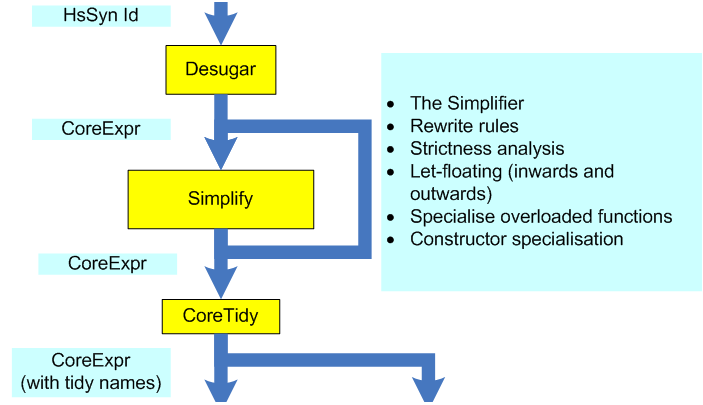
\includegraphics[scale=0.4]{images/HscPipe2_2.png}
\caption{Compiler Teil 2 \copyright haskell.org}
\end{figure}
\end{frame}

\begin{frame}
\frametitle{Interne Funktionsweise}
\begin{figure}
\centering
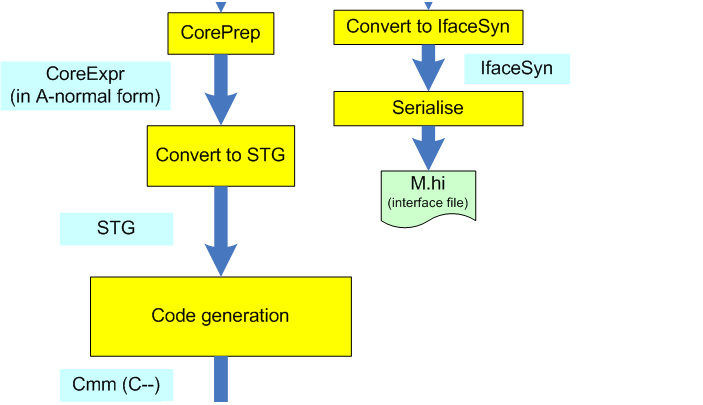
\includegraphics[scale=0.4]{images/HscPipe2_3.png}
\caption{Compiler Teil 3 \copyright haskell.org}
\end{figure}
\end{frame}

\begin{frame}
\frametitle{Interne Funktionsweise}
\begin{figure}
\centering
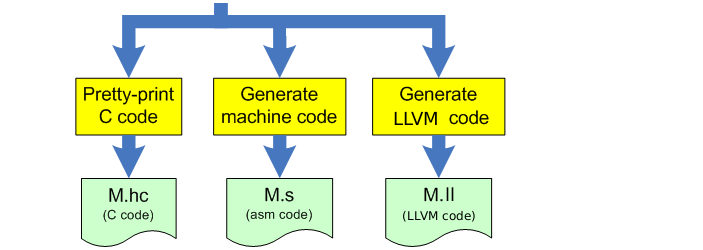
\includegraphics[scale=0.4]{images/HscPipe2_4.png}
\caption{Compiler Teil 4 \copyright haskell.org}
\end{figure}
\end{frame}

\section{Semantische Grundbegriffe}

\subsection{Namen und Attribute}
\begin{frame}
\frametitle{Namen und Attribute}
\begin{block}{\vspace*{-3ex}}
\begin{itemize}
  \item Alle endlichen ASCII-Strings außer:
  \\ \lstinline|case|, \lstinline|class|, \lstinline|data|, \lstinline|default|, \lstinline|deriving|, \lstinline|do|, \lstinline|else|, \lstinline|if|, \lstinline|import|, \lstinline|in|, \lstinline|infix|, \lstinline|infixl|, \lstinline|infixr|, \lstinline|instance|, \lstinline|let|, \lstinline|module|, \lstinline|newtype|, \lstinline|of|, \lstinline|then|, \lstinline|type|, \lstinline|where|
  \item Bezeichner sind case-sensitiv. (\lstinline|pLus| $\neq$ \lstinline|plus|) 
  \item \lstinline|_| (Unterstrich) ist der Platzhalter
  \item Module beginnen mit einem Großbuchstaben
  \item Funktionen mit einem Kleinbuchstaben
\end{itemize}
\end{block}
\end{frame}

\subsection{Variablen und Konstanten}
\begin{frame}
\frametitle{Variablen}
\begin{block}{\vspace*{-3ex}}
\begin{itemize}
  \item Globale Variablen existieren nicht
  \item Lokale Variablen existieren nur in Funktionen als Teilergebnis
\end{itemize}
\end{block}
\end{frame}

\begin{frame}
\frametitle{Konstanten}
\begin{block}{\vspace*{-3ex}}
%\begin{itemize}
%  \item Konstanten sind Funktionen ohne Parameter
%\end{itemize}
Konstanten sind Funktionen ohne Parameter
\end{block}
\end{frame}

\subsection{Ausdrücke}
\begin{frame}
\frametitle{Ausdrücke}
\begin{block}{\vspace*{-3ex}}
elementare Ausdrücke bzw. Grundterme setzten sich zusammen aus:
\begin{itemize}
  \item Konstanten wie z.B. Zahlen (\lstinline|10|, \lstinline|9.8|), Zeichen (\lstinline|'a'|, \lstinline|'Z'|), \ldots
  \item Andere Funktionen \lstinline|sin|, \lstinline|+|, \lstinline|*|, \ldots
\end{itemize}
\end{block}
\begin{alertblock}{Infixnotation}
Funktionszeichen: \lstinline|3 + 4| $\equiv$ \lstinline|(+) 3 4|\\
Funktionsname: \lstinline|mod 100 4| $\equiv$ \lstinline|100 `mod` 4|
\end{alertblock}
\end{frame}

\begin{frame}
\frametitle{Ausdrücke}
\begin{block}{\vspace*{-3ex}}
\begin{itemize}
  \item Elementare Ausdrücke mit Variablen sind Ausdrücke bzw. Terme
  \item Durch einen "`Vorspann"' wie $\ x$ wird die Variable $x$ mit der $\lambda$-Notation "`gebunden"'
  \item $\lambda a \to \lambda b \to a + b$ ist ein $\lambda$-Ausdruck
  \item $\lambda$ ist kein ASCII Zeichen, deswegen wird "`\textbackslash"' verwendet 
\end{itemize}
\end{block}
\end{frame}

\begin{frame}[fragile]
\frametitle{Ausdrücke} 
\begin{exampleblock}{Elementarer Ausdruck}
\lstinline|plus = 10 + 30|
\end{exampleblock}
\begin{exampleblock}{Ausdruck}
\lstinline|plus' a b = a + b|
\end{exampleblock}
\begin{exampleblock}{Lambda ($\lambda$)-Ausdruck}
\lstinline|plus'' =  \a -> \b -> a + b|\\
Morgen kommt mehr zum Thema $\lambda$-Ausdrücke
\end{exampleblock}
\end{frame}

\subsection{Funktionen}
\begin{frame}
\frametitle{Deklaration von Funktionen}
\begin{block}{\vspace*{-3ex}}
\begin{itemize}
  \item Funktion $f$ ist ein Tripel $(D_f, W_f, R_f)$
  \item $D_f$ Definitionsmenge
  \item $W_f$ Wertemenge
  \item $R_f \subseteq D_f \times W_f$
  \item $R_f$ muss \textbf{rechtseindeutig} sein d.h. es gibt keine zwei Paare $(a,b1) \in R_f$ und $(a,b_2) \in R_f$ mit $b_1 \neq b_2$
  \item Somit gilt, eine Funktion $f$ bildet den Argumentwert $x$ in den Resultatwert $y$ ab 
\end{itemize}
\end{block}
\end{frame}

\begin{frame}
\frametitle{Deklaration von Funktionen}
\only<1>{
\vspace*{-1ex}
\begin{exampleblock}{Konstante}
\begin{center}
\scalebox{0.6}{\begin{tikzpicture}[
      nonterminal/.style={
         rectangle,
         minimum size=5.0mm,
         very thick,
         draw=blue!50!black!50,
         top color=white,
         bottom color=blue!50!black!20,
         font=\itshape\scriptsize,
         %text height=1.5ex,
         %text depth=.25ex
      },
      terminal/.style={
         rounded rectangle,
         minimum size=5.0mm,
         very thick,draw=black!50,
         top color=white,bottom color=black!20,
         font=\ttfamily\scriptsize,
         %text height=1.5ex,
         %text depth=.25ex
      },
      skip loop/.style={
         to path={-- ++(0,#1) -| (\tikztotarget)}
      },
      point/.style={coordinate},>=stealth',thick,draw=black!50,
      tip/.style={->,shorten >=0.007pt},every join/.style={rounded corners},
      hv path/.style={to path={-| (\tikztotarget)}},
      vh path/.style={to path={|- (\tikztotarget)}},
      %text height=1.5ex,text depth=.25ex
    ]
    \matrix[column sep=5.0mm, row sep=3.0mm] {
 &  & \node (n13) [nonterminal] {Bezeichner}; & \node (n14) [terminal] {::}; & \node (n15) [nonterminal] {Typ Erg}; & \node (n16) [terminal] {LF}; &  & \\
\node (n21) [circle, draw, inner sep=0pt, minimum size=0.75ex] {}; & \node (n22) [point] {}; &  &  &  &  & \node (n27) [point] {}; & \node (n28) [point] {};\\
 &  & \node (n33) [point] {}; &  &  &  &  & \\
 &  &  &  &  &  &  & \\
 &  &  &  & \node (n55) [nonterminal] {Wert}; &  &  & \\
\node (n61) [point] {}; & \node (n62) [nonterminal] {Bezeichner}; & \node (n63) [terminal] {=}; & \node (n64) [point] {}; &  & \node (n66) [point] {}; & \node (n67) [terminal] {LF}; & \node (n68) [circle, draw, inner sep=0pt, minimum size=0.75ex] {};\\
 &  &  &  & \node (n75) [nonterminal] {Ausdruck}; &  &  & \\
    };
  { [start chain]
       \chainin (n21);
       \chainin (n22)    [join];
  }
  { [start chain]
       \chainin (n22);
       \chainin (n13)    [join=by {vh path,tip}];
  }
  { [start chain]
       \chainin (n13);
       \chainin (n14)    [join=by tip];
  }
  { [start chain]
       \chainin (n14);
       \chainin (n15)    [join=by tip];
  }
  { [start chain]
       \chainin (n15);
       \chainin (n16)    [join=by tip];
  }
  { [start chain]
       \chainin (n16);
       \chainin (n27)    [join=by {hv path}];
  }
  { [start chain]
       \chainin (n22);
       \chainin (n33)    [join=by {vh path}];
  }
  { [start chain]
       \chainin (n33);
       \chainin (n27)    [join=by {hv path}];
  }
  { [start chain]
       \chainin (n27);
       \chainin (n28)    [join=by tip];
  }
  { [start chain]
       \chainin (n61);
       \chainin (n62)    [join=by tip];
  }
  { [start chain]
       \chainin (n62);
       \chainin (n63)    [join=by tip];
  }
  { [start chain]
       \chainin (n63);
       \chainin (n64)    [join];
  }
  { [start chain]
       \chainin (n64);
       \chainin (n55)    [join=by {vh path,tip}];
  }
  { [start chain]
       \chainin (n55);
       \chainin (n66)    [join=by {hv path}];
  }
  { [start chain]
       \chainin (n64);
       \chainin (n75)    [join=by {vh path,tip}];
  }
  { [start chain]
       \chainin (n75);
       \chainin (n66)    [join=by {hv path}];
  }
  { [start chain]
       \chainin (n66);
       \chainin (n67)    [join=by tip];
  }
  { [start chain]
       \chainin (n67);
       \chainin (n68)    [join=by tip];
  }
\end{tikzpicture}
}
\end{center}
\end{exampleblock}}
\only<2>{
\vspace*{-1ex}
\begin{exampleblock}{Funktion}
\begin{center}
\scalebox{0.5}{\begin{tikzpicture}[
      nonterminal/.style={
         rectangle,
         minimum size=5.0mm,
         very thick,
         draw=blue!50!black!50,
         top color=white,
         bottom color=blue!50!black!20,
         font=\itshape\scriptsize,
         %text height=1.5ex,
         %text depth=.25ex
      },
      terminal/.style={
         rounded rectangle,
         minimum size=5.0mm,
         very thick,draw=black!50,
         top color=white,bottom color=black!20,
         font=\ttfamily\scriptsize,
         %text height=1.5ex,
         %text depth=.25ex
      },
      skip loop/.style={
         to path={-- ++(0,#1) -| (\tikztotarget)}
      },
      point/.style={coordinate},>=stealth',thick,draw=black!50,
      tip/.style={->,shorten >=0.007pt},every join/.style={rounded corners},
      hv path/.style={to path={-| (\tikztotarget)}},
      vh path/.style={to path={|- (\tikztotarget)}},
      %text height=1.5ex,text depth=.25ex
    ]
    \matrix[column sep=5.0mm, row sep=3.0mm] {
 &  &  &  &  & \node (n16) [point] {}; &  &  &  &  &  &  & \\
 &  & \node (n23) [nonterminal] {Bezeichner}; & \node (n24) [terminal] {::}; & \node (n25) [point] {}; & \node (n26) [nonterminal] {Typ Para}; & \node (n27) [terminal] {->}; & \node (n28) [point] {}; & \node (n29) [nonterminal] {Typ Erg}; & \node (n210) [terminal] {LF}; &  &  & \\
\node (n31) [circle, draw, inner sep=0pt, minimum size=0.75ex] {}; & \node (n32) [point] {}; &  &  &  &  &  &  &  &  & \node (n311) [point] {}; & \node (n312) [point] {}; & \\
 &  & \node (n43) [point] {}; &  &  &  &  &  &  &  &  &  & \\
 &  &  &  &  &  &  &  &  &  &  &  & \\
 &  &  &  &  &  & \node (n67) [point] {}; &  &  &  &  &  & \\
 &  &  &  & \node (n75) [point] {}; &  &  &  & \node (n79) [nonterminal] {Wert}; &  &  &  & \\
\node (n81) [point] {}; & \node (n82) [point] {}; & \node (n83) [nonterminal] {Bezeichner}; & \node (n84) [point] {}; & \node (n85) [nonterminal] {Bezeichner Para}; & \node (n86) [point] {}; & \node (n87) [terminal] {=}; & \node (n88) [point] {}; &  & \node (n810) [point] {}; & \node (n811) [terminal] {LF}; & \node (n812) [point] {}; & \node (n813) [circle, draw, inner sep=0pt, minimum size=0.75ex] {};\\
 &  &  &  &  &  &  &  & \node (n99) [nonterminal] {Ausdruck}; &  &  &  & \\
    };
  { [start chain]
       \chainin (n31);
       \chainin (n32)    [join];
  }
  { [start chain]
       \chainin (n32);
       \chainin (n23)    [join=by {vh path,tip}];
  }
  { [start chain]
       \chainin (n23);
       \chainin (n24)    [join=by tip];
  }
  { [start chain]
       \chainin (n24);
       \chainin (n25)    [join];
  }
  { [start chain]
       \chainin (n25);
       \chainin (n26)    [join=by tip];
  }
  { [start chain]
       \chainin (n26);
       \chainin (n27)    [join=by tip];
  }
  { [start chain]
       \chainin (n27);
       \chainin (n28)    [join];
  }
  { [start chain]
       \chainin (n28);
       \chainin (n29)    [join=by tip];
  }
  { [start chain]
       \chainin (n29);
       \chainin (n210)    [join=by tip];
  }
  { [start chain]
       \chainin (n210);
       \chainin (n311)    [join=by {hv path}];
  }
  { [start chain]
       \chainin (n32);
       \chainin (n43)    [join=by {vh path}];
  }
  { [start chain]
       \chainin (n43);
       \chainin (n311)    [join=by {hv path}];
  }
  { [start chain]
       \chainin (n311);
       \chainin (n312)    [join=by tip];
  }
  { [start chain]
       \chainin (n81);
       \chainin (n82)    [join];
  }
  { [start chain]
       \chainin (n82);
       \chainin (n83)    [join=by tip];
  }
  { [start chain]
       \chainin (n83);
       \chainin (n84)    [join];
  }
  { [start chain]
       \chainin (n84);
       \chainin (n85)    [join=by tip];
  }
  { [start chain]
       \chainin (n85);
       \chainin (n86)    [join];
  }
  { [start chain]
       \chainin (n86);
       \chainin (n87)    [join=by tip];
  }
  { [start chain]
       \chainin (n87);
       \chainin (n88)    [join];
  }
  { [start chain]
       \chainin (n88);
       \chainin (n79)    [join=by {vh path,tip}];
  }
  { [start chain]
       \chainin (n79);
       \chainin (n810)    [join=by {hv path}];
  }
  { [start chain]
       \chainin (n88);
       \chainin (n99)    [join=by {vh path,tip}];
  }
  { [start chain]
       \chainin (n99);
       \chainin (n810)    [join=by {hv path}];
  }
  { [start chain]
       \chainin (n810);
       \chainin (n811)    [join=by tip];
  }
  { [start chain]
       \chainin (n811);
       \chainin (n812)    [join];
  }
  { [start chain]
       \chainin (n812);
       \chainin (n813)    [join=by tip];
  }
  { [start chain]
       \chainin (n28);
       \chainin (n16)    [join=by vh path];
       \chainin (n25)    [join=by {hv path,tip}];
  }
  { [start chain]
       \chainin (n86);
       \chainin (n75)    [join=by vh path];
       \chainin (n84)    [join=by {hv path,tip}];
  }
  { [start chain]
       \chainin (n812);
       \chainin (n67)    [join=by vh path];
       \chainin (n82)    [join=by {hv path,tip}];
  }
\end{tikzpicture}
}
\end{center}
\end{exampleblock}}
\only<3>{\begin{exampleblock}{Allgemein}
\begin{center}
\scalebox{0.6}{\begin{tikzpicture}[
      nonterminal/.style={
         rectangle,
         minimum size=5.0mm,
         very thick,
         draw=blue!50!black!50,
         top color=white,
         bottom color=blue!50!black!20,
         font=\itshape\scriptsize,
         %text height=1.5ex,
         %text depth=.25ex
      },
      terminal/.style={
         rounded rectangle,
         minimum size=5.0mm,
         very thick,draw=black!50,
         top color=white,bottom color=black!20,
         font=\ttfamily\scriptsize,
         %text height=1.5ex,
         %text depth=.25ex
      },
      skip loop/.style={
         to path={-- ++(0,#1) -| (\tikztotarget)}
      },
      point/.style={coordinate},>=stealth',thick,draw=black!50,
      tip/.style={->,shorten >=0.007pt},every join/.style={rounded corners},
      hv path/.style={to path={-| (\tikztotarget)}},
      vh path/.style={to path={|- (\tikztotarget)}},
      %text height=1.5ex,text depth=.25ex
    ]
    \matrix[column sep=5.0mm, row sep=3.0mm] {
 &  &  &  &  & \node (n16) [terminal] {->}; & \node (n17) [nonterminal] {Typ Para}; &  &  &  &  &  & \\
 &  & \node (n23) [nonterminal] {Bezeichner}; & \node (n24) [terminal] {::}; & \node (n25) [point] {}; &  &  & \node (n28) [point] {}; & \node (n29) [nonterminal] {Typ Erg}; & \node (n210) [terminal] {LF}; &  &  & \\
\node (n31) [circle, draw, inner sep=0pt, minimum size=0.75ex] {}; & \node (n32) [point] {}; &  &  &  &  &  &  &  &  & \node (n311) [point] {}; & \node (n312) [point] {}; & \\
 &  & \node (n43) [point] {}; &  &  &  &  &  &  &  &  &  & \\
 &  &  &  &  &  &  &  &  &  &  &  & \\
 &  &  &  &  &  & \node (n67) [point] {}; &  &  &  &  &  & \\
 &  &  &  & \node (n75) [nonterminal] {Bezeichner Para}; &  &  &  & \node (n79) [nonterminal] {Wert}; &  &  &  & \\
\node (n81) [point] {}; & \node (n82) [point] {}; & \node (n83) [nonterminal] {Bezeichner}; & \node (n84) [point] {}; &  & \node (n86) [point] {}; & \node (n87) [terminal] {=}; & \node (n88) [point] {}; &  & \node (n810) [point] {}; & \node (n811) [terminal] {LF}; & \node (n812) [point] {}; & \node (n813) [circle, draw, inner sep=0pt, minimum size=0.75ex] {};\\
 &  &  &  &  &  &  &  & \node (n99) [nonterminal] {Ausdruck}; &  &  &  & \\
    };
  { [start chain]
       \chainin (n31);
       \chainin (n32)    [join];
  }
  { [start chain]
       \chainin (n32);
       \chainin (n23)    [join=by {vh path,tip}];
  }
  { [start chain]
       \chainin (n23);
       \chainin (n24)    [join=by tip];
  }
  { [start chain]
       \chainin (n24);
       \chainin (n25)    [join];
  }
  { [start chain]
       \chainin (n25);
       \chainin (n28)    [join];
  }
  { [start chain]
       \chainin (n17);
       \chainin (n16)    [join=by tip];
  }
  { [start chain]
       \chainin (n28);
       \chainin (n17)    [join=by {vh path,tip}];
  }
  { [start chain]
       \chainin (n16);
       \chainin (n25)    [join=by {hv path,tip}];
  }
  { [start chain]
       \chainin (n28);
       \chainin (n29)    [join=by tip];
  }
  { [start chain]
       \chainin (n29);
       \chainin (n210)    [join=by tip];
  }
  { [start chain]
       \chainin (n210);
       \chainin (n311)    [join=by {hv path}];
  }
  { [start chain]
       \chainin (n32);
       \chainin (n43)    [join=by {vh path}];
  }
  { [start chain]
       \chainin (n43);
       \chainin (n311)    [join=by {hv path}];
  }
  { [start chain]
       \chainin (n311);
       \chainin (n312)    [join=by tip];
  }
  { [start chain]
       \chainin (n81);
       \chainin (n82)    [join];
  }
  { [start chain]
       \chainin (n82);
       \chainin (n83)    [join=by tip];
  }
  { [start chain]
       \chainin (n83);
       \chainin (n84)    [join];
  }
  { [start chain]
       \chainin (n84);
       \chainin (n86)    [join];
  }
  { [start chain]
       \chainin (n86);
       \chainin (n75)    [join=by {vh path,tip}];
  }
  { [start chain]
       \chainin (n75);
       \chainin (n84)    [join=by {hv path,tip}];
  }
  { [start chain]
       \chainin (n86);
       \chainin (n87)    [join=by tip];
  }
  { [start chain]
       \chainin (n87);
       \chainin (n88)    [join];
  }
  { [start chain]
       \chainin (n88);
       \chainin (n79)    [join=by {vh path,tip}];
  }
  { [start chain]
       \chainin (n79);
       \chainin (n810)    [join=by {hv path}];
  }
  { [start chain]
       \chainin (n88);
       \chainin (n99)    [join=by {vh path,tip}];
  }
  { [start chain]
       \chainin (n99);
       \chainin (n810)    [join=by {hv path}];
  }
  { [start chain]
       \chainin (n810);
       \chainin (n811)    [join=by tip];
  }
  { [start chain]
       \chainin (n811);
       \chainin (n812)    [join];
  }
  { [start chain]
       \chainin (n812);
       \chainin (n813)    [join=by tip];
  }
  { [start chain]
       \chainin (n812);
       \chainin (n67)    [join=by vh path];
       \chainin (n82)    [join=by {hv path,tip}];
  }
\end{tikzpicture}
}
\end{center}
\end{exampleblock}}
\only<1-2>{\vspace*{-3ex}
\begin{block}{\vspace*{-3ex}}
\begin{itemize} 
  \item Funktionsköpfe sind optional, jedoch empfohlen
  \item Funktionsnamen beginnen mit Kleinbuchstaben
  \item Parameter von Funktionen beginnen mit Kleinbuchstaben
\end{itemize}
\end{block}}
\end{frame}

\begin{frame}[fragile]
\frametitle{Deklaration von Funktionen} 
\begin{exampleblock}{Konstante}
\begin{lstlisting}
eins :: Int
eins  = 1
\end{lstlisting}
\end{exampleblock}
\end{frame}

\begin{frame}[fragile]
\frametitle{Deklaration von Funktionen} 
\begin{exampleblock}{Konstante}
\begin{lstlisting}
eins :: Int
eins  = 1
\end{lstlisting}
\end{exampleblock}
\begin{exampleblock}{Unäre Funktion}
\begin{lstlisting}
successor :: Int -> Int
successor      a  = a + 1
\end{lstlisting}
\end{exampleblock}
\end{frame}

\begin{frame}[fragile]
\frametitle{Deklaration von Funktionen} 
\vspace*{-2.5ex}
\begin{exampleblock}{Konstante}
\begin{lstlisting}
eins :: Int
eins  = 1
\end{lstlisting}
\end{exampleblock}
\vspace*{-3ex}
\begin{exampleblock}{Unäre Funktion}
\begin{lstlisting}
successor :: Int -> Int
successor      a  = a + 1
\end{lstlisting}
\end{exampleblock}
\vspace*{-3ex}
\begin{exampleblock}{Binäre Funktion}
\begin{lstlisting}
nimmDenZweiten :: Int -> Int -> Int
nimmDenZweiten    _      b    = b
\end{lstlisting}
\end{exampleblock}
\end{frame}

\begin{frame}
\frametitle{Funktionen vs. Operatoren}
\begin{block}{\vspace*{-3ex}}
\begin{itemize}
  \item Funktionen besitzen einen Namen aus Buchstaben
  \item Operatoren besitzen einen Namen aus Zeichen
  \item Funktionen binden stärker als Operatoren (Standard)
  \item Operatoren werden wie Funktionen deklariert
\end{itemize}
\end{block}
\end{frame}

\subsection{Blöcke}
\begin{frame}
\frametitle{Der where Block}
\vspace*{-3ex}
\begin{block}{\vspace*{-3ex}}
\begin{itemize}
  \item Zur nachträglichen Definition von internen Hilfsfunktionen (Teilfunktionen)
  %\item {}<ober Funktion> \dots = <Hilfsfunktion> + <Ausdruck> \\ \textbf{where} \\ <Hilfsfunktion> \dots = \dots
  \item Verschachtelung erlaubt
  \item Definiert für die ganze Funktion
  \item "`Funktionsköpfe"' erlaubt
\end{itemize}
\end{block}
\only<2>{
\vspace*{-2ex}
	\begin{exampleblock}{\vspace*{-3ex}}
	\begin{center}
	\vspace*{-2ex}
	\scalebox{0.45}{\begin{tikzpicture}[
      nonterminal/.style={
         rectangle,
         minimum size=5.0mm,
         very thick,
         draw=blue!50!black!50,
         top color=white,
         bottom color=blue!50!black!20,
         font=\itshape\scriptsize,
         %text height=1.5ex,
         %text depth=.25ex
      },
      terminal/.style={
         rounded rectangle,
         minimum size=5.0mm,
         very thick,draw=black!50,
         top color=white,bottom color=black!20,
         font=\ttfamily\scriptsize,
         %text height=1.5ex,
         %text depth=.25ex
      },
      skip loop/.style={
         to path={-- ++(0,#1) -| (\tikztotarget)}
      },
      point/.style={coordinate},>=stealth',thick,draw=black!50,
      tip/.style={->,shorten >=0.007pt},every join/.style={rounded corners},
      hv path/.style={to path={-| (\tikztotarget)}},
      vh path/.style={to path={|- (\tikztotarget)}},
      %text height=1.5ex,text depth=.25ex
    ]
    \matrix[column sep=5.0mm, row sep=3.0mm] {
 &  &  &  &  &  &  &  & \node (n19) [point] {}; &  &  &  &  &  &  &  &  &  &  & \\
 &  &  & \node (n24) [point] {}; &  &  &  &  & \node (n29) [nonterminal] {Ausdruck}; &  &  &  &  &  &  &  &  &  &  & \\
\node (n31) [circle, draw, inner sep=0pt, minimum size=0.75ex] {}; & \node (n32) [nonterminal] {Funktion}; & \node (n33) [point] {}; & \node (n34) [nonterminal] {Parameter}; & \node (n35) [point] {}; & \node (n36) [terminal] {=}; & \node (n37) [point] {}; & \node (n38) [point] {}; &  & \node (n310) [point] {}; & \node (n311) [point] {}; & \node (n312) [terminal] {LF}; & \node (n313) [point] {}; &  &  &  &  &  &  & \\
 &  &  &  &  &  &  &  & \node (n49) [nonterminal] {Hilfsfunktion}; &  &  &  &  &  &  &  &  &  &  & \\
 &  &  &  &  &  &  &  &  &  &  &  &  &  &  &  &  &  &  & \\
 &  &  &  &  &  &  &  &  & \node (n610) [point] {}; &  &  &  &  &  &  &  &  &  & \\
 &  &  &  &  &  &  &  &  &  &  & \node (n712) [point] {}; &  &  &  &  &  &  &  & \\
 &  &  &  &  &  &  &  &  &  &  &  &  & \node (n814) [point] {}; &  &  &  &  &  & \\
 &  &  &  &  &  &  &  & \node (n99) [point] {}; &  &  &  &  & \node (n914) [nonterminal] {Ausdruck}; &  &  &  &  &  & \\
\node (n101) [point] {}; & \node (n102) [point] {}; & \node (n103) [terminal] {Tab}; & \node (n104) [terminal] {where}; & \node (n105) [terminal] {LF}; & \node (n106) [point] {}; & \node (n107) [nonterminal] {Hilfsfunktion}; & \node (n108) [point] {}; & \node (n109) [nonterminal] {Parameter}; & \node (n1010) [point] {}; & \node (n1011) [terminal] {=}; & \node (n1012) [point] {}; & \node (n1013) [point] {}; &  & \node (n1015) [point] {}; & \node (n1016) [point] {}; & \node (n1017) [terminal] {LF}; & \node (n1018) [point] {}; & \node (n1019) [point] {}; & \node (n1020) [circle, draw, inner sep=0pt, minimum size=0.75ex] {};\\
 &  &  &  &  &  &  &  &  &  &  &  &  & \node (n1114) [nonterminal] {Hilfsfunktion}; &  &  &  &  &  & \\
    };
  { [start chain]
       \chainin (n31);
       \chainin (n32)    [join=by tip];
  }
  { [start chain]
       \chainin (n32);
       \chainin (n33)    [join];
  }
  { [start chain]
       \chainin (n33);
       \chainin (n34)    [join=by tip];
  }
  { [start chain]
       \chainin (n34);
       \chainin (n35)    [join];
  }
  { [start chain]
       \chainin (n35);
       \chainin (n36)    [join=by tip];
  }
  { [start chain]
       \chainin (n36);
       \chainin (n37)    [join];
  }
  { [start chain]
       \chainin (n37);
       \chainin (n38)    [join];
  }
  { [start chain]
       \chainin (n38);
       \chainin (n29)    [join=by {vh path,tip}];
  }
  { [start chain]
       \chainin (n29);
       \chainin (n310)    [join=by {hv path}];
  }
  { [start chain]
       \chainin (n38);
       \chainin (n49)    [join=by {vh path,tip}];
  }
  { [start chain]
       \chainin (n49);
       \chainin (n310)    [join=by {hv path}];
  }
  { [start chain]
       \chainin (n310);
       \chainin (n311)    [join];
  }
  { [start chain]
       \chainin (n311);
       \chainin (n312)    [join=by tip];
  }
  { [start chain]
       \chainin (n312);
       \chainin (n313)    [join=by tip];
  }
  { [start chain]
       \chainin (n101);
       \chainin (n102)    [join];
  }
  { [start chain]
       \chainin (n102);
       \chainin (n103)    [join=by tip];
  }
  { [start chain]
       \chainin (n103);
       \chainin (n104)    [join=by tip];
  }
  { [start chain]
       \chainin (n104);
       \chainin (n105)    [join=by tip];
  }
  { [start chain]
       \chainin (n105);
       \chainin (n106)    [join];
  }
  { [start chain]
       \chainin (n106);
       \chainin (n107)    [join=by tip];
  }
  { [start chain]
       \chainin (n107);
       \chainin (n108)    [join];
  }
  { [start chain]
       \chainin (n108);
       \chainin (n109)    [join=by tip];
  }
  { [start chain]
       \chainin (n109);
       \chainin (n1010)    [join];
  }
  { [start chain]
       \chainin (n1010);
       \chainin (n1011)    [join=by tip];
  }
  { [start chain]
       \chainin (n1011);
       \chainin (n1012)    [join];
  }
  { [start chain]
       \chainin (n1012);
       \chainin (n1013)    [join];
  }
  { [start chain]
       \chainin (n1013);
       \chainin (n914)    [join=by {vh path,tip}];
  }
  { [start chain]
       \chainin (n914);
       \chainin (n1015)    [join=by {hv path}];
  }
  { [start chain]
       \chainin (n1013);
       \chainin (n1114)    [join=by {vh path,tip}];
  }
  { [start chain]
       \chainin (n1114);
       \chainin (n1015)    [join=by {hv path}];
  }
  { [start chain]
       \chainin (n1015);
       \chainin (n1016)    [join];
  }
  { [start chain]
       \chainin (n1016);
       \chainin (n1017)    [join=by tip];
  }
  { [start chain]
       \chainin (n1017);
       \chainin (n1018)    [join];
  }
  { [start chain]
       \chainin (n1018);
       \chainin (n1019)    [join];
  }
  { [start chain]
       \chainin (n1019);
       \chainin (n1020)    [join=by tip];
  }
  { [start chain]
       \chainin (n35);
       \chainin (n24)    [join=by vh path];
       \chainin (n33)    [join=by {hv path,tip}];
  }
  { [start chain]
       \chainin (n311);
       \chainin (n19)    [join=by vh path];
       \chainin (n37)    [join=by {hv path,tip}];
  }
  { [start chain]
       \chainin (n1010);
       \chainin (n99)    [join=by vh path];
       \chainin (n108)    [join=by {hv path,tip}];
  }
  { [start chain]
       \chainin (n1016);
       \chainin (n814)    [join=by vh path];
       \chainin (n1012)    [join=by {hv path,tip}];
  }
  { [start chain]
       \chainin (n1018);
       \chainin (n712)    [join=by vh path];
       \chainin (n106)    [join=by {hv path,tip}];
  }
  { [start chain]
       \chainin (n1019);
       \chainin (n610)    [join=by vh path];
       \chainin (n102)    [join=by {hv path,tip}];
  }
\end{tikzpicture}
}
	\end{center}
	\end{exampleblock}
}
\end{frame}

\begin{frame}[fragile]
\frametitle{Der where Block}
\begin{lstlisting}
dec a = inc a - 2
    where	
        inc a = a + 1
\end{lstlisting}
\begin{exampleblock}{\vspace*{-3ex}}
\begin{center}
\vspace*{-1ex}
\scalebox{0.45}{\begin{tikzpicture}[
      nonterminal/.style={
         rectangle,
         minimum size=5.0mm,
         very thick,
         draw=blue!50!black!50,
         top color=white,
         bottom color=blue!50!black!20,
         font=\itshape\scriptsize,
         %text height=1.5ex,
         %text depth=.25ex
      },
      terminal/.style={
         rounded rectangle,
         minimum size=5.0mm,
         very thick,draw=black!50,
         top color=white,bottom color=black!20,
         font=\ttfamily\scriptsize,
         %text height=1.5ex,
         %text depth=.25ex
      },
      skip loop/.style={
         to path={-- ++(0,#1) -| (\tikztotarget)}
      },
      point/.style={coordinate},>=stealth',thick,draw=black!50,
      tip/.style={->,shorten >=0.007pt},every join/.style={rounded corners},
      hv path/.style={to path={-| (\tikztotarget)}},
      vh path/.style={to path={|- (\tikztotarget)}},
      %text height=1.5ex,text depth=.25ex
    ]
    \matrix[column sep=5.0mm, row sep=3.0mm] {
 &  &  &  &  &  &  &  & \node (n19) [point] {}; &  &  &  &  &  &  &  &  &  &  & \\
 &  &  & \node (n24) [point] {}; &  &  &  &  & \node (n29) [nonterminal] {Ausdruck}; &  &  &  &  &  &  &  &  &  &  & \\
\node (n31) [circle, draw, inner sep=0pt, minimum size=0.75ex] {}; & \node (n32) [nonterminal] {Funktion}; & \node (n33) [point] {}; & \node (n34) [nonterminal] {Parameter}; & \node (n35) [point] {}; & \node (n36) [terminal] {=}; & \node (n37) [point] {}; & \node (n38) [point] {}; &  & \node (n310) [point] {}; & \node (n311) [point] {}; & \node (n312) [terminal] {LF}; & \node (n313) [point] {}; &  &  &  &  &  &  & \\
 &  &  &  &  &  &  &  & \node (n49) [nonterminal] {Hilfsfunktion}; &  &  &  &  &  &  &  &  &  &  & \\
 &  &  &  &  &  &  &  &  &  &  &  &  &  &  &  &  &  &  & \\
 &  &  &  &  &  &  &  &  & \node (n610) [point] {}; &  &  &  &  &  &  &  &  &  & \\
 &  &  &  &  &  &  &  &  &  &  & \node (n712) [point] {}; &  &  &  &  &  &  &  & \\
 &  &  &  &  &  &  &  &  &  &  &  &  & \node (n814) [point] {}; &  &  &  &  &  & \\
 &  &  &  &  &  &  &  & \node (n99) [point] {}; &  &  &  &  & \node (n914) [nonterminal] {Ausdruck}; &  &  &  &  &  & \\
\node (n101) [point] {}; & \node (n102) [point] {}; & \node (n103) [terminal] {Tab}; & \node (n104) [terminal] {where}; & \node (n105) [terminal] {LF}; & \node (n106) [point] {}; & \node (n107) [nonterminal] {Hilfsfunktion}; & \node (n108) [point] {}; & \node (n109) [nonterminal] {Parameter}; & \node (n1010) [point] {}; & \node (n1011) [terminal] {=}; & \node (n1012) [point] {}; & \node (n1013) [point] {}; &  & \node (n1015) [point] {}; & \node (n1016) [point] {}; & \node (n1017) [terminal] {LF}; & \node (n1018) [point] {}; & \node (n1019) [point] {}; & \node (n1020) [circle, draw, inner sep=0pt, minimum size=0.75ex] {};\\
 &  &  &  &  &  &  &  &  &  &  &  &  & \node (n1114) [nonterminal] {Hilfsfunktion}; &  &  &  &  &  & \\
    };
  { [start chain]
       \chainin (n31);
       \chainin (n32)    [join=by tip];
  }
  { [start chain]
       \chainin (n32);
       \chainin (n33)    [join];
  }
  { [start chain]
       \chainin (n33);
       \chainin (n34)    [join=by tip];
  }
  { [start chain]
       \chainin (n34);
       \chainin (n35)    [join];
  }
  { [start chain]
       \chainin (n35);
       \chainin (n36)    [join=by tip];
  }
  { [start chain]
       \chainin (n36);
       \chainin (n37)    [join];
  }
  { [start chain]
       \chainin (n37);
       \chainin (n38)    [join];
  }
  { [start chain]
       \chainin (n38);
       \chainin (n29)    [join=by {vh path,tip}];
  }
  { [start chain]
       \chainin (n29);
       \chainin (n310)    [join=by {hv path}];
  }
  { [start chain]
       \chainin (n38);
       \chainin (n49)    [join=by {vh path,tip}];
  }
  { [start chain]
       \chainin (n49);
       \chainin (n310)    [join=by {hv path}];
  }
  { [start chain]
       \chainin (n310);
       \chainin (n311)    [join];
  }
  { [start chain]
       \chainin (n311);
       \chainin (n312)    [join=by tip];
  }
  { [start chain]
       \chainin (n312);
       \chainin (n313)    [join=by tip];
  }
  { [start chain]
       \chainin (n101);
       \chainin (n102)    [join];
  }
  { [start chain]
       \chainin (n102);
       \chainin (n103)    [join=by tip];
  }
  { [start chain]
       \chainin (n103);
       \chainin (n104)    [join=by tip];
  }
  { [start chain]
       \chainin (n104);
       \chainin (n105)    [join=by tip];
  }
  { [start chain]
       \chainin (n105);
       \chainin (n106)    [join];
  }
  { [start chain]
       \chainin (n106);
       \chainin (n107)    [join=by tip];
  }
  { [start chain]
       \chainin (n107);
       \chainin (n108)    [join];
  }
  { [start chain]
       \chainin (n108);
       \chainin (n109)    [join=by tip];
  }
  { [start chain]
       \chainin (n109);
       \chainin (n1010)    [join];
  }
  { [start chain]
       \chainin (n1010);
       \chainin (n1011)    [join=by tip];
  }
  { [start chain]
       \chainin (n1011);
       \chainin (n1012)    [join];
  }
  { [start chain]
       \chainin (n1012);
       \chainin (n1013)    [join];
  }
  { [start chain]
       \chainin (n1013);
       \chainin (n914)    [join=by {vh path,tip}];
  }
  { [start chain]
       \chainin (n914);
       \chainin (n1015)    [join=by {hv path}];
  }
  { [start chain]
       \chainin (n1013);
       \chainin (n1114)    [join=by {vh path,tip}];
  }
  { [start chain]
       \chainin (n1114);
       \chainin (n1015)    [join=by {hv path}];
  }
  { [start chain]
       \chainin (n1015);
       \chainin (n1016)    [join];
  }
  { [start chain]
       \chainin (n1016);
       \chainin (n1017)    [join=by tip];
  }
  { [start chain]
       \chainin (n1017);
       \chainin (n1018)    [join];
  }
  { [start chain]
       \chainin (n1018);
       \chainin (n1019)    [join];
  }
  { [start chain]
       \chainin (n1019);
       \chainin (n1020)    [join=by tip];
  }
  { [start chain]
       \chainin (n35);
       \chainin (n24)    [join=by vh path];
       \chainin (n33)    [join=by {hv path,tip}];
  }
  { [start chain]
       \chainin (n311);
       \chainin (n19)    [join=by vh path];
       \chainin (n37)    [join=by {hv path,tip}];
  }
  { [start chain]
       \chainin (n1010);
       \chainin (n99)    [join=by vh path];
       \chainin (n108)    [join=by {hv path,tip}];
  }
  { [start chain]
       \chainin (n1016);
       \chainin (n814)    [join=by vh path];
       \chainin (n1012)    [join=by {hv path,tip}];
  }
  { [start chain]
       \chainin (n1018);
       \chainin (n712)    [join=by vh path];
       \chainin (n106)    [join=by {hv path,tip}];
  }
  { [start chain]
       \chainin (n1019);
       \chainin (n610)    [join=by vh path];
       \chainin (n102)    [join=by {hv path,tip}];
  }
\end{tikzpicture}
}
\end{center}
\end{exampleblock}
\end{frame}

\begin{frame}[fragile]
\frametitle{Der where Block}
\begin{lstlisting}
f :: Int -> Int 
f   a   = x a `div` 3
    where x b = y b * 2
        where y b = a + b + 1 
\end{lstlisting}
\only<1>{
\begin{exampleblock}{\vspace*{-3ex}}
\begin{center}
\vspace*{-1ex}
\scalebox{0.45}{\begin{tikzpicture}[
      nonterminal/.style={
         rectangle,
         minimum size=5.0mm,
         very thick,
         draw=blue!50!black!50,
         top color=white,
         bottom color=blue!50!black!20,
         font=\itshape\scriptsize,
         %text height=1.5ex,
         %text depth=.25ex
      },
      terminal/.style={
         rounded rectangle,
         minimum size=5.0mm,
         very thick,draw=black!50,
         top color=white,bottom color=black!20,
         font=\ttfamily\scriptsize,
         %text height=1.5ex,
         %text depth=.25ex
      },
      skip loop/.style={
         to path={-- ++(0,#1) -| (\tikztotarget)}
      },
      point/.style={coordinate},>=stealth',thick,draw=black!50,
      tip/.style={->,shorten >=0.007pt},every join/.style={rounded corners},
      hv path/.style={to path={-| (\tikztotarget)}},
      vh path/.style={to path={|- (\tikztotarget)}},
      %text height=1.5ex,text depth=.25ex
    ]
    \matrix[column sep=5.0mm, row sep=3.0mm] {
 &  &  &  &  &  &  &  & \node (n19) [point] {}; &  &  &  &  &  &  &  &  &  &  & \\
 &  &  & \node (n24) [point] {}; &  &  &  &  & \node (n29) [nonterminal] {Ausdruck}; &  &  &  &  &  &  &  &  &  &  & \\
\node (n31) [circle, draw, inner sep=0pt, minimum size=0.75ex] {}; & \node (n32) [nonterminal] {Funktion}; & \node (n33) [point] {}; & \node (n34) [nonterminal] {Parameter}; & \node (n35) [point] {}; & \node (n36) [terminal] {=}; & \node (n37) [point] {}; & \node (n38) [point] {}; &  & \node (n310) [point] {}; & \node (n311) [point] {}; & \node (n312) [terminal] {LF}; & \node (n313) [point] {}; &  &  &  &  &  &  & \\
 &  &  &  &  &  &  &  & \node (n49) [nonterminal] {Hilfsfunktion}; &  &  &  &  &  &  &  &  &  &  & \\
 &  &  &  &  &  &  &  &  &  &  &  &  &  &  &  &  &  &  & \\
 &  &  &  &  &  &  &  &  & \node (n610) [point] {}; &  &  &  &  &  &  &  &  &  & \\
 &  &  &  &  &  &  &  &  &  &  & \node (n712) [point] {}; &  &  &  &  &  &  &  & \\
 &  &  &  &  &  &  &  &  &  &  &  &  & \node (n814) [point] {}; &  &  &  &  &  & \\
 &  &  &  &  &  &  &  & \node (n99) [point] {}; &  &  &  &  & \node (n914) [nonterminal] {Ausdruck}; &  &  &  &  &  & \\
\node (n101) [point] {}; & \node (n102) [point] {}; & \node (n103) [terminal] {Tab}; & \node (n104) [terminal] {where}; & \node (n105) [terminal] {LF}; & \node (n106) [point] {}; & \node (n107) [nonterminal] {Hilfsfunktion}; & \node (n108) [point] {}; & \node (n109) [nonterminal] {Parameter}; & \node (n1010) [point] {}; & \node (n1011) [terminal] {=}; & \node (n1012) [point] {}; & \node (n1013) [point] {}; &  & \node (n1015) [point] {}; & \node (n1016) [point] {}; & \node (n1017) [terminal] {LF}; & \node (n1018) [point] {}; & \node (n1019) [point] {}; & \node (n1020) [circle, draw, inner sep=0pt, minimum size=0.75ex] {};\\
 &  &  &  &  &  &  &  &  &  &  &  &  & \node (n1114) [nonterminal] {Hilfsfunktion}; &  &  &  &  &  & \\
    };
  { [start chain]
       \chainin (n31);
       \chainin (n32)    [join=by tip];
  }
  { [start chain]
       \chainin (n32);
       \chainin (n33)    [join];
  }
  { [start chain]
       \chainin (n33);
       \chainin (n34)    [join=by tip];
  }
  { [start chain]
       \chainin (n34);
       \chainin (n35)    [join];
  }
  { [start chain]
       \chainin (n35);
       \chainin (n36)    [join=by tip];
  }
  { [start chain]
       \chainin (n36);
       \chainin (n37)    [join];
  }
  { [start chain]
       \chainin (n37);
       \chainin (n38)    [join];
  }
  { [start chain]
       \chainin (n38);
       \chainin (n29)    [join=by {vh path,tip}];
  }
  { [start chain]
       \chainin (n29);
       \chainin (n310)    [join=by {hv path}];
  }
  { [start chain]
       \chainin (n38);
       \chainin (n49)    [join=by {vh path,tip}];
  }
  { [start chain]
       \chainin (n49);
       \chainin (n310)    [join=by {hv path}];
  }
  { [start chain]
       \chainin (n310);
       \chainin (n311)    [join];
  }
  { [start chain]
       \chainin (n311);
       \chainin (n312)    [join=by tip];
  }
  { [start chain]
       \chainin (n312);
       \chainin (n313)    [join=by tip];
  }
  { [start chain]
       \chainin (n101);
       \chainin (n102)    [join];
  }
  { [start chain]
       \chainin (n102);
       \chainin (n103)    [join=by tip];
  }
  { [start chain]
       \chainin (n103);
       \chainin (n104)    [join=by tip];
  }
  { [start chain]
       \chainin (n104);
       \chainin (n105)    [join=by tip];
  }
  { [start chain]
       \chainin (n105);
       \chainin (n106)    [join];
  }
  { [start chain]
       \chainin (n106);
       \chainin (n107)    [join=by tip];
  }
  { [start chain]
       \chainin (n107);
       \chainin (n108)    [join];
  }
  { [start chain]
       \chainin (n108);
       \chainin (n109)    [join=by tip];
  }
  { [start chain]
       \chainin (n109);
       \chainin (n1010)    [join];
  }
  { [start chain]
       \chainin (n1010);
       \chainin (n1011)    [join=by tip];
  }
  { [start chain]
       \chainin (n1011);
       \chainin (n1012)    [join];
  }
  { [start chain]
       \chainin (n1012);
       \chainin (n1013)    [join];
  }
  { [start chain]
       \chainin (n1013);
       \chainin (n914)    [join=by {vh path,tip}];
  }
  { [start chain]
       \chainin (n914);
       \chainin (n1015)    [join=by {hv path}];
  }
  { [start chain]
       \chainin (n1013);
       \chainin (n1114)    [join=by {vh path,tip}];
  }
  { [start chain]
       \chainin (n1114);
       \chainin (n1015)    [join=by {hv path}];
  }
  { [start chain]
       \chainin (n1015);
       \chainin (n1016)    [join];
  }
  { [start chain]
       \chainin (n1016);
       \chainin (n1017)    [join=by tip];
  }
  { [start chain]
       \chainin (n1017);
       \chainin (n1018)    [join];
  }
  { [start chain]
       \chainin (n1018);
       \chainin (n1019)    [join];
  }
  { [start chain]
       \chainin (n1019);
       \chainin (n1020)    [join=by tip];
  }
  { [start chain]
       \chainin (n35);
       \chainin (n24)    [join=by vh path];
       \chainin (n33)    [join=by {hv path,tip}];
  }
  { [start chain]
       \chainin (n311);
       \chainin (n19)    [join=by vh path];
       \chainin (n37)    [join=by {hv path,tip}];
  }
  { [start chain]
       \chainin (n1010);
       \chainin (n99)    [join=by vh path];
       \chainin (n108)    [join=by {hv path,tip}];
  }
  { [start chain]
       \chainin (n1016);
       \chainin (n814)    [join=by vh path];
       \chainin (n1012)    [join=by {hv path,tip}];
  }
  { [start chain]
       \chainin (n1018);
       \chainin (n712)    [join=by vh path];
       \chainin (n106)    [join=by {hv path,tip}];
  }
  { [start chain]
       \chainin (n1019);
       \chainin (n610)    [join=by vh path];
       \chainin (n102)    [join=by {hv path,tip}];
  }
\end{tikzpicture}
}
\end{center}
\end{exampleblock}}
\only<2-3>{
\begin{exampleblock}{Aufruf}
\lstinline|f 4|
\end{exampleblock}}
\only<3>{
\begin{exampleblock}{Ausgabe}
\lstinline|6|
\end{exampleblock}}
\end{frame}

\begin{frame}
\frametitle{Der let-in Block}
\only<1>{\begin{block}{\vspace*{-3ex}}
\begin{itemize}
  \item Zur vorherigen Definition von internen Hilfsfunktionen (Teilfunktionen)
  %\item {[} <ober Funktion> \dots = {]} \\ \textbf{let} <Hilfsfunktion> \dots = \dots \\ {[}\textbf{in} 
  % <Hilfsfunktion> + <Ausdruck> {]}
  \item Kann auch zur Definition von Funktionen im Interpreter verwendet werden  
  \item Verschachtelung erlaubt
  \item Definiert für den Funktionsabschnitt 
\end{itemize}
\end{block}}
\only<2>{\begin{exampleblock}{\vspace*{-3ex}}
\begin{center}
\scalebox{0.45}{\begin{tikzpicture}[
      nonterminal/.style={
         rectangle,
         minimum size=5.0mm,
         very thick,
         draw=blue!50!black!50,
         top color=white,
         bottom color=blue!50!black!20,
         font=\itshape\scriptsize,
         %text height=1.5ex,
         %text depth=.25ex
      },
      terminal/.style={
         rounded rectangle,
         minimum size=5.0mm,
         very thick,draw=black!50,
         top color=white,bottom color=black!20,
         font=\ttfamily\scriptsize,
         %text height=1.5ex,
         %text depth=.25ex
      },
      skip loop/.style={
         to path={-- ++(0,#1) -| (\tikztotarget)}
      },
      point/.style={coordinate},>=stealth',thick,draw=black!50,
      tip/.style={->,shorten >=0.007pt},every join/.style={rounded corners},
      hv path/.style={to path={-| (\tikztotarget)}},
      vh path/.style={to path={|- (\tikztotarget)}},
      %text height=1.5ex,text depth=.25ex
    ]
    \matrix[column sep=5.0mm, row sep=3.0mm] {
 &  &  & \node (n14) [point] {}; &  &  &  &  &  &  &  &  &  &  &  &  &  & \\
\node (n21) [circle, draw, inner sep=0pt, minimum size=0.75ex] {}; & \node (n22) [nonterminal] {Funktion}; & \node (n23) [point] {}; & \node (n24) [nonterminal] {Parameter}; & \node (n25) [point] {}; & \node (n26) [terminal] {=}; & \node (n27) [terminal] {LF}; & \node (n28) [point] {}; &  &  &  &  &  &  &  &  &  & \\
 &  &  &  &  &  &  &  &  &  &  &  &  &  &  &  &  & \\
 &  &  &  &  &  &  &  &  &  & \node (n411) [point] {}; &  &  &  &  &  &  & \\
 &  &  &  &  &  &  &  &  &  &  &  & \node (n513) [point] {}; &  &  &  &  & \\
 &  &  &  &  &  &  & \node (n68) [point] {}; &  &  &  &  & \node (n613) [nonterminal] {Ausdruck}; &  &  &  &  & \\
\node (n71) [point] {}; & \node (n72) [terminal] {Tab}; & \node (n73) [terminal] {let}; & \node (n74) [terminal] {LF}; & \node (n75) [point] {}; & \node (n76) [nonterminal] {Hilfsfunktion}; & \node (n77) [point] {}; & \node (n78) [nonterminal] {Parameter}; & \node (n79) [point] {}; & \node (n710) [terminal] {=}; & \node (n711) [point] {}; & \node (n712) [point] {}; &  & \node (n714) [point] {}; & \node (n715) [point] {}; & \node (n716) [terminal] {LF}; & \node (n717) [point] {}; & \node (n718) [point] {};\\
 &  &  &  &  &  &  &  &  &  &  &  & \node (n813) [nonterminal] {TiefereHilfsfunktion}; &  &  &  &  & \\
 &  &  &  &  &  &  &  &  &  &  &  &  &  &  &  &  & \\
 &  &  & \node (n104) [nonterminal] {Ausdruck}; &  &  &  &  &  &  &  &  &  &  &  &  &  & \\
\node (n111) [point] {}; & \node (n112) [terminal] {in}; & \node (n113) [point] {}; &  & \node (n115) [point] {}; & \node (n116) [circle, draw, inner sep=0pt, minimum size=0.75ex] {}; &  &  &  &  &  &  &  &  &  &  &  & \\
 &  &  & \node (n124) [nonterminal] {Hilfsfunktion}; &  &  &  &  &  &  &  &  &  &  &  &  &  & \\
    };
  { [start chain]
       \chainin (n21);
       \chainin (n22)    [join=by tip];
  }
  { [start chain]
       \chainin (n22);
       \chainin (n23)    [join];
  }
  { [start chain]
       \chainin (n23);
       \chainin (n24)    [join=by tip];
  }
  { [start chain]
       \chainin (n24);
       \chainin (n25)    [join];
  }
  { [start chain]
       \chainin (n25);
       \chainin (n26)    [join=by tip];
  }
  { [start chain]
       \chainin (n26);
       \chainin (n27)    [join=by tip];
  }
  { [start chain]
       \chainin (n27);
       \chainin (n28)    [join=by tip];
  }
  { [start chain]
       \chainin (n71);
       \chainin (n72)    [join=by tip];
  }
  { [start chain]
       \chainin (n72);
       \chainin (n73)    [join=by tip];
  }
  { [start chain]
       \chainin (n73);
       \chainin (n74)    [join=by tip];
  }
  { [start chain]
       \chainin (n74);
       \chainin (n75)    [join];
  }
  { [start chain]
       \chainin (n75);
       \chainin (n76)    [join=by tip];
  }
  { [start chain]
       \chainin (n76);
       \chainin (n77)    [join];
  }
  { [start chain]
       \chainin (n77);
       \chainin (n78)    [join=by tip];
  }
  { [start chain]
       \chainin (n78);
       \chainin (n79)    [join];
  }
  { [start chain]
       \chainin (n79);
       \chainin (n710)    [join=by tip];
  }
  { [start chain]
       \chainin (n710);
       \chainin (n711)    [join];
  }
  { [start chain]
       \chainin (n711);
       \chainin (n712)    [join];
  }
  { [start chain]
       \chainin (n712);
       \chainin (n613)    [join=by {vh path,tip}];
  }
  { [start chain]
       \chainin (n613);
       \chainin (n714)    [join=by {hv path}];
  }
  { [start chain]
       \chainin (n712);
       \chainin (n813)    [join=by {vh path,tip}];
  }
  { [start chain]
       \chainin (n813);
       \chainin (n714)    [join=by {hv path}];
  }
  { [start chain]
       \chainin (n714);
       \chainin (n715)    [join];
  }
  { [start chain]
       \chainin (n715);
       \chainin (n716)    [join=by tip];
  }
  { [start chain]
       \chainin (n716);
       \chainin (n717)    [join];
  }
  { [start chain]
       \chainin (n717);
       \chainin (n718)    [join=by tip];
  }
  { [start chain]
       \chainin (n111);
       \chainin (n112)    [join=by tip];
  }
  { [start chain]
       \chainin (n112);
       \chainin (n113)    [join];
  }
  { [start chain]
       \chainin (n113);
       \chainin (n104)    [join=by {vh path,tip}];
  }
  { [start chain]
       \chainin (n104);
       \chainin (n115)    [join=by {hv path}];
  }
  { [start chain]
       \chainin (n113);
       \chainin (n124)    [join=by {vh path,tip}];
  }
  { [start chain]
       \chainin (n124);
       \chainin (n115)    [join=by {hv path}];
  }
  { [start chain]
       \chainin (n115);
       \chainin (n116)    [join=by tip];
  }
  { [start chain]
       \chainin (n25);
       \chainin (n14)    [join=by vh path];
       \chainin (n23)    [join=by {hv path,tip}];
  }
  { [start chain]
       \chainin (n79);
       \chainin (n68)    [join=by vh path];
       \chainin (n77)    [join=by {hv path,tip}];
  }
  { [start chain]
       \chainin (n715);
       \chainin (n513)    [join=by vh path];
       \chainin (n711)    [join=by {hv path,tip}];
  }
  { [start chain]
       \chainin (n717);
       \chainin (n411)    [join=by vh path];
       \chainin (n75)    [join=by {hv path,tip}];
  }
\end{tikzpicture}
}\\
Blöcke mit let-in können verschachtelt sein
\end{center}
\end{exampleblock}}
\end{frame}

\begin{frame}[fragile]
\frametitle{Der let-in Block}
\begin{lstlisting}
dec a = 
  let inc1 a = a + 1
      inc2 a = a + 2
  in  inc1 a - inc2 0
\end{lstlisting}
\only<1>{\begin{exampleblock}{Zur Definition von Funktionen direkt im GHCi}
\lstinline|let {plus :: Int -> Int -> Int; plus a b = a + b}|
\end{exampleblock}}
\only<2-3>{
\begin{exampleblock}{Aufruf}
\lstinline|dec 42|
\end{exampleblock}}
\only<3>{
\begin{exampleblock}{Ausgabe}
\lstinline|41|
\end{exampleblock}}
\end{frame}

\begin{frame}[fragile]
\frametitle{Der let-in Block}
\begin{lstlisting}
outer a = 
    let mid b = 
        let inner c = c + 1
        in inner b + 2
    in mid a + 3	
\end{lstlisting}
\only<1-2>{
\begin{exampleblock}{Aufruf}
\lstinline|outer 42|
\end{exampleblock}}
\only<2>{
\begin{exampleblock}{Ausgabe}
\lstinline|48|
\end{exampleblock}}
\end{frame}

\section{Einfache Datentypen}
\begin{frame}
\frametitle{Einfache Datentypen}
\begin{block}{\vspace*{-3ex}}
\begin{itemize}
  \item \lstinline|Bool|
  \item \lstinline|Int|
  \item \lstinline|Integer|
  \item \lstinline|Float|
  \item \lstinline|Double|
  \item \lstinline|Char|
\end{itemize}
\end{block}
\end{frame}
\subsection{Warheitswerte}
\begin{frame}
\frametitle{\lstinline|Bool|}
\begin{block}{\vspace*{-3ex}}
\begin{itemize}
  \item Einfacher Wahrheitswert
  \item \lstinline|True| oder \lstinline|False|
  \item \lstinline|not| $\equiv$ Verneinung
  \item \lstinline|&&| (binär), \lstinline|and| (Liste) $\equiv$ und
  \item \lstinline!||! (binär), \lstinline|or| (Liste) $\equiv$ oder
  \item \lstinline|==| $\equiv$ gleich
  \item \lstinline|/=| $\equiv$ ungleich
\end{itemize}
\end{block}
\end{frame}

\begin{frame}[fragile]
\frametitle{\lstinline|Bool|} 
\begin{lstlisting}
myAnd :: Bool -> Bool -> Bool
myAnd True True  = True
myAnd _    _     = False

myOr :: Bool -> Bool -> Bool
myOr False False = False
myOr _     _     = True
\end{lstlisting}
\end{frame}
\subsection{Ganzzahlen}
\begin{frame}
\frametitle{\lstinline|Int|}
\begin{block}{\vspace*{-3ex}}
\begin{itemize}
  \item 32 Bit Ganzzahl (Architektur abhängig)
  \item Min = $-2^{31} = -2147483648$
  \item Max = $2^{31} - 1 = 2147483647$
  \item Zirkulär $(2^{31} - 1) + 1 = -2^{31}$ 
\end{itemize}
\end{block}
\begin{alertblock}{Achtung}
\lstinline|Int| ist nicht gleich \lstinline|Integer|!
\end{alertblock}
\end{frame}

\begin{frame}
\frametitle{\lstinline|Integer|}
\begin{block}{\vspace*{-3ex}}
\begin{itemize}
  \item Unbegrenzte Ganzzahl (RAM Größe ist die "`Begrenzung"')
  \item Bei unendlich Arbeitsspeicher wirklich unbegrenzt
\end{itemize}
\end{block}
\end{frame}

\begin{frame}[fragile]
\frametitle{\lstinline|Int| vs \lstinline|Integer|} 
\begin{lstlisting}
plus :: Int -> Int -> Int
plus a b = a + b
\end{lstlisting}
\only<1-2>{
\begin{exampleblock}{Aufruf}
\lstinline|plus 2147483647 1|
\end{exampleblock}}
\only<2>{
\begin{exampleblock}{Ausgabe}
\lstinline|-2147483648|
\end{exampleblock}}
\end{frame}

\begin{frame}[fragile]
\frametitle{\lstinline|Int| vs \lstinline|Integer|} 
\begin{lstlisting}
plus' :: Integer -> Integer -> Integer
plus' a b = a + b
\end{lstlisting}
\only<1-2>{
\begin{exampleblock}{Aufruf}
\lstinline|plus' 9876543210 9876543210|
\end{exampleblock}}
\only<2>{
\begin{exampleblock}{Ausgabe}
\lstinline|19753086420|
\end{exampleblock}}
\only<3-4>{
\begin{exampleblock}{Aufruf}
\lstinline|plus' 99999999999999999999 99999999999999999999|
\end{exampleblock}}
\only<4>{
\begin{exampleblock}{Ausgabe}
\lstinline|199999999999999999998|
\end{exampleblock}}
\end{frame}

\begin{frame}[fragile]
\frametitle{\lstinline|Int| vs \lstinline|Integer|} 
\begin{lstlisting}
id :: Int -> Integer
id a = a

id' :: Integer -> Int
id' a = a
\end{lstlisting}
\begin{alertblock}{Geht nicht}
Auch wenn \lstinline|Int| für uns eine Teilmenge von \lstinline|Integer| ist.
\end{alertblock}
\end{frame}

\begin{frame}[fragile]
\frametitle{\lstinline|Int| vs \lstinline|Integer|} 
\begin{lstlisting}
plus :: Integer -> Int -> Integer
plus a 0 = a
plus a b = plus (a + 1) (b - 1)

plus' :: Int -> Integer -> Int
plus' a 0 = a
plus' a b = plus' (a + 1) (b - 1)
\end{lstlisting}
\begin{alertblock}{Geht}
Jedoch hat dies nichts mit interner Typkompatibilität zu tun.
\end{alertblock}
\end{frame}

\subsection{Gleitkommazahl}
\begin{frame}
\frametitle{\lstinline|Float| - \lstinline|Double|}
\begin{block}{\vspace*{-3ex}}
\begin{itemize}
  \item \lstinline|Float| 32 Bit Gleitkommazahl 
  \item \lstinline|Double| 64 Bit Gleitkommazahl
  \item \lstinline|Float| und \lstinline|Double| sind ebenfalls inkompatibel zueinander wie \lstinline|Int| und \lstinline|Integer|
\end{itemize}
\end{block}
\end{frame}

\subsection{Zeichen}
\begin{frame}
\frametitle{\lstinline|Char|}
\begin{block}{\vspace*{-3ex}}
\begin{itemize}
  \item Stellt jedes Zeichen des Unicode (ISO 10646) da
  \item Geordnet nach der Reihenfolge des Auftretens
\end{itemize}
\end{block}
\end{frame}
% % % % % % % % % % % % % % % % % % % % %
\part{Tag zwei}
\tocm
\subtitle{Tag zwei - etwas mehr} 
\date{25.03.2014}

\begin{frame}[plain]
\titlepage
\end{frame}
\section{Currying - allgemein}
\begin{frame}
\frametitle{Deklaration von Funktionen in $\lambda$ Notation}
\only<1-3>{
\vspace*{-2ex}
	\begin{block}{Lambda Currying}
	\begin{center}
	$f = \lambda x_1 \to \lambda x_2 \to \dots \lambda x_n \to e$
	\end{center}
	\end{block}
}
\only<2-3>{
\vspace*{-3ex}
	\begin{exampleblock}{Funkion Currying}
	\begin{center}
	\scalebox{0.6}{\begin{tikzpicture}[
      nonterminal/.style={
         rectangle,
         minimum size=5.0mm,
         very thick,
         draw=blue!50!black!50,
         top color=white,
         bottom color=blue!50!black!20,
         font=\itshape\scriptsize,
         %text height=1.5ex,
         %text depth=.25ex
      },
      terminal/.style={
         rounded rectangle,
         minimum size=5.0mm,
         very thick,draw=black!50,
         top color=white,bottom color=black!20,
         font=\ttfamily\scriptsize,
         %text height=1.5ex,
         %text depth=.25ex
      },
      skip loop/.style={
         to path={-- ++(0,#1) -| (\tikztotarget)}
      },
      point/.style={coordinate},>=stealth',thick,draw=black!50,
      tip/.style={->,shorten >=0.007pt},every join/.style={rounded corners},
      hv path/.style={to path={-| (\tikztotarget)}},
      vh path/.style={to path={|- (\tikztotarget)}},
      %text height=1.5ex,text depth=.25ex
    ]
    \matrix[column sep=5.0mm, row sep=3.0mm] {
 &  &  &  & \node (n15) [point] {}; &  &  & \\
\node (n21) [circle, draw, inner sep=0pt, minimum size=0.75ex] {}; & \node (n22) [nonterminal] {Bezeichner}; & \node (n23) [terminal] {=}; & \node (n24) [point] {}; & \node (n25) [nonterminal] {Parameter}; & \node (n26) [point] {}; & \node (n27) [nonterminal] {Ausdruck}; & \node (n28) [circle, draw, inner sep=0pt, minimum size=0.75ex] {};\\
    };
  { [start chain]
       \chainin (n21);
       \chainin (n22)    [join=by tip];
  }
  { [start chain]
       \chainin (n22);
       \chainin (n23)    [join=by tip];
  }
  { [start chain]
       \chainin (n23);
       \chainin (n24)    [join];
  }
  { [start chain]
       \chainin (n24);
       \chainin (n25)    [join=by tip];
  }
  { [start chain]
       \chainin (n25);
       \chainin (n26)    [join];
  }
  { [start chain]
       \chainin (n26);
       \chainin (n27)    [join=by tip];
  }
  { [start chain]
       \chainin (n27);
       \chainin (n28)    [join=by tip];
  }
  { [start chain]
       \chainin (n26);
       \chainin (n15)    [join=by vh path];
       \chainin (n24)    [join=by {hv path,tip}];
  }
\end{tikzpicture}
}
	\end{center}
	\end{exampleblock}
}
\only<3>{
\vspace*{-3ex}
	\begin{exampleblock}{Lambda Currying}
	\begin{center}
	\scalebox{0.6}{\begin{tikzpicture}[
      nonterminal/.style={
         rectangle,
         minimum size=5.0mm,
         very thick,
         draw=blue!50!black!50,
         top color=white,
         bottom color=blue!50!black!20,
         font=\itshape\scriptsize,
         %text height=1.5ex,
         %text depth=.25ex
      },
      terminal/.style={
         rounded rectangle,
         minimum size=5.0mm,
         very thick,draw=black!50,
         top color=white,bottom color=black!20,
         font=\ttfamily\scriptsize,
         %text height=1.5ex,
         %text depth=.25ex
      },
      skip loop/.style={
         to path={-- ++(0,#1) -| (\tikztotarget)}
      },
      point/.style={coordinate},>=stealth',thick,draw=black!50,
      tip/.style={->,shorten >=0.007pt},every join/.style={rounded corners},
      hv path/.style={to path={-| (\tikztotarget)}},
      vh path/.style={to path={|- (\tikztotarget)}},
      %text height=1.5ex,text depth=.25ex
    ]
    \matrix[column sep=5.0mm, row sep=3.0mm] {
 &  & \node (n13) [point] {}; &  &  &  &  & \node (n18) [point] {}; &  &  &  & \\
\node (n21) [circle, draw, inner sep=0pt, minimum size=0.75ex] {}; & \node (n22) [point] {}; & \node (n23) [nonterminal] {Bezeichner}; & \node (n24) [terminal] {=}; & \node (n25) [point] {}; & \node (n26) [point] {}; & \node (n27) [terminal] {$\lambda$}; & \node (n28) [nonterminal] {Parameter}; & \node (n29) [terminal] {->}; & \node (n210) [point] {}; & \node (n211) [nonterminal] {Ausdruck}; & \node (n212) [circle, draw, inner sep=0pt, minimum size=0.75ex] {};\\
    };
  { [start chain]
       \chainin (n21);
       \chainin (n22)    [join];
  }
  { [start chain]
       \chainin (n22);
       \chainin (n23)    [join=by tip];
  }
  { [start chain]
       \chainin (n23);
       \chainin (n24)    [join=by tip];
  }
  { [start chain]
       \chainin (n24);
       \chainin (n25)    [join];
  }
  { [start chain]
       \chainin (n25);
       \chainin (n26)    [join];
  }
  { [start chain]
       \chainin (n26);
       \chainin (n27)    [join=by tip];
  }
  { [start chain]
       \chainin (n27);
       \chainin (n28)    [join=by tip];
  }
  { [start chain]
       \chainin (n28);
       \chainin (n29)    [join=by tip];
  }
  { [start chain]
       \chainin (n29);
       \chainin (n210)    [join];
  }
  { [start chain]
       \chainin (n210);
       \chainin (n211)    [join=by tip];
  }
  { [start chain]
       \chainin (n211);
       \chainin (n212)    [join=by tip];
  }
  { [start chain]
       \chainin (n22);
       \chainin (n13)    [join=by vh path];
       \chainin (n25)    [join=by {hv path,tip}];
  }
  { [start chain]
       \chainin (n210);
       \chainin (n18)    [join=by vh path];
       \chainin (n26)    [join=by {hv path,tip}];
  }
\end{tikzpicture}
}
	\end{center}
	\end{exampleblock}
}
\end{frame}

\begin{frame}
\frametitle{Deklaration von Funktionen in $\lambda$ Notation}
\only<1-3>{
\vspace*{-2ex}
	\begin{block}{Lambda Uncurrying}
	\begin{center}
	$f = \lambda(x_1, x_2, \dots, x_n) \to e$
	\end{center}
	\end{block}
}
\only<2-3>{
\vspace*{-3ex}
	\begin{exampleblock}{Funkion Uncurrying}
	\begin{center}
	\scalebox{0.6}{\begin{tikzpicture}[
      nonterminal/.style={
         rectangle,
         minimum size=5.0mm,
         very thick,
         draw=blue!50!black!50,
         top color=white,
         bottom color=blue!50!black!20,
         font=\itshape\scriptsize,
         %text height=1.5ex,
         %text depth=.25ex
      },
      terminal/.style={
         rounded rectangle,
         minimum size=5.0mm,
         very thick,draw=black!50,
         top color=white,bottom color=black!20,
         font=\ttfamily\scriptsize,
         %text height=1.5ex,
         %text depth=.25ex
      },
      skip loop/.style={
         to path={-- ++(0,#1) -| (\tikztotarget)}
      },
      point/.style={coordinate},>=stealth',thick,draw=black!50,
      tip/.style={->,shorten >=0.007pt},every join/.style={rounded corners},
      hv path/.style={to path={-| (\tikztotarget)}},
      vh path/.style={to path={|- (\tikztotarget)}},
      %text height=1.5ex,text depth=.25ex
    ]
    \matrix[column sep=5.0mm, row sep=3.0mm] {
 &  &  &  &  & \node (n16) [nonterminal] {Parameter}; & \node (n17) [terminal] {,}; &  &  &  &  & \\
\node (n21) [circle, draw, inner sep=0pt, minimum size=0.75ex] {}; & \node (n22) [nonterminal] {Bezeichner}; & \node (n23) [terminal] {(}; & \node (n24) [nonterminal] {Parameter}; & \node (n25) [point] {}; &  &  & \node (n28) [point] {}; & \node (n29) [terminal] {)}; & \node (n210) [terminal] {=}; & \node (n211) [nonterminal] {Ausdruck}; & \node (n212) [circle, draw, inner sep=0pt, minimum size=0.75ex] {};\\
    };
  { [start chain]
       \chainin (n21);
       \chainin (n22)    [join=by tip];
  }
  { [start chain]
       \chainin (n22);
       \chainin (n23)    [join=by tip];
  }
  { [start chain]
       \chainin (n23);
       \chainin (n24)    [join=by tip];
  }
  { [start chain]
       \chainin (n24);
       \chainin (n25)    [join];
  }
  { [start chain]
       \chainin (n25);
       \chainin (n28)    [join];
  }
  { [start chain]
       \chainin (n16);
       \chainin (n17)    [join=by tip];
  }
  { [start chain]
       \chainin (n28);
       \chainin (n17)    [join=by {vh path,tip}];
  }
  { [start chain]
       \chainin (n16);
       \chainin (n25)    [join=by {hv path,tip}];
  }
  { [start chain]
       \chainin (n28);
       \chainin (n29)    [join=by tip];
  }
  { [start chain]
       \chainin (n29);
       \chainin (n210)    [join=by tip];
  }
  { [start chain]
       \chainin (n210);
       \chainin (n211)    [join=by tip];
  }
  { [start chain]
       \chainin (n211);
       \chainin (n212)    [join=by tip];
  }
\end{tikzpicture}
}
	\end{center}
	\end{exampleblock}
}
\only<2>{
	\begin{alertblock}{ABER}
	Das Tupel $(x_1, x_2, \dots, x_n)$ ist ein eigener Datentyp
	\end{alertblock}
}
\only<3>{
\vspace*{-3ex}
	\begin{exampleblock}{Lambda Uncurrying}
	\begin{center}
	\scalebox{0.6}{\begin{tikzpicture}[
      nonterminal/.style={
         rectangle,
         minimum size=5.0mm,
         very thick,
         draw=blue!50!black!50,
         top color=white,
         bottom color=blue!50!black!20,
         font=\itshape\scriptsize,
         %text height=1.5ex,
         %text depth=.25ex
      },
      terminal/.style={
         rounded rectangle,
         minimum size=5.0mm,
         very thick,draw=black!50,
         top color=white,bottom color=black!20,
         font=\ttfamily\scriptsize,
         %text height=1.5ex,
         %text depth=.25ex
      },
      skip loop/.style={
         to path={-- ++(0,#1) -| (\tikztotarget)}
      },
      point/.style={coordinate},>=stealth',thick,draw=black!50,
      tip/.style={->,shorten >=0.007pt},every join/.style={rounded corners},
      hv path/.style={to path={-| (\tikztotarget)}},
      vh path/.style={to path={|- (\tikztotarget)}},
      %text height=1.5ex,text depth=.25ex
    ]
    \matrix[column sep=5.0mm, row sep=3.0mm] {
 &  & \node (n13) [point] {}; &  &  &  &  &  &  & \node (n110) [nonterminal] {Parameter}; & \node (n111) [terminal] {,}; &  &  &  &  & \\
\node (n21) [circle, draw, inner sep=0pt, minimum size=0.75ex] {}; & \node (n22) [point] {}; & \node (n23) [nonterminal] {Bezeichner}; & \node (n24) [terminal] {=}; & \node (n25) [point] {}; & \node (n26) [terminal] {$\lambda$}; & \node (n27) [terminal] {(}; & \node (n28) [nonterminal] {Parameter}; & \node (n29) [point] {}; &  &  & \node (n212) [point] {}; & \node (n213) [terminal] {)}; & \node (n214) [terminal] {->}; & \node (n215) [nonterminal] {Ausdruck}; & \node (n216) [circle, draw, inner sep=0pt, minimum size=0.75ex] {};\\
    };
  { [start chain]
       \chainin (n21);
       \chainin (n22)    [join];
  }
  { [start chain]
       \chainin (n22);
       \chainin (n23)    [join=by tip];
  }
  { [start chain]
       \chainin (n23);
       \chainin (n24)    [join=by tip];
  }
  { [start chain]
       \chainin (n24);
       \chainin (n25)    [join];
  }
  { [start chain]
       \chainin (n25);
       \chainin (n26)    [join=by tip];
  }
  { [start chain]
       \chainin (n26);
       \chainin (n27)    [join=by tip];
  }
  { [start chain]
       \chainin (n27);
       \chainin (n28)    [join=by tip];
  }
  { [start chain]
       \chainin (n28);
       \chainin (n29)    [join];
  }
  { [start chain]
       \chainin (n29);
       \chainin (n212)    [join];
  }
  { [start chain]
       \chainin (n111);
       \chainin (n110)    [join=by tip];
  }
  { [start chain]
       \chainin (n212);
       \chainin (n111)    [join=by {vh path,tip}];
  }
  { [start chain]
       \chainin (n110);
       \chainin (n29)    [join=by {hv path,tip}];
  }
  { [start chain]
       \chainin (n212);
       \chainin (n213)    [join=by tip];
  }
  { [start chain]
       \chainin (n213);
       \chainin (n214)    [join=by tip];
  }
  { [start chain]
       \chainin (n214);
       \chainin (n215)    [join=by tip];
  }
  { [start chain]
       \chainin (n215);
       \chainin (n216)    [join=by tip];
  }
  { [start chain]
       \chainin (n22);
       \chainin (n13)    [join=by vh path];
       \chainin (n25)    [join=by {hv path,tip}];
  }
\end{tikzpicture}
}
	\end{center}
	\end{exampleblock}
}
\end{frame}

\begin{frame}[fragile]
\frametitle{Deklaration von Funktionen} 	
%\begin{block}{\vspace*{-3ex}}
\begin{lstlisting}
plus :: Int -> Int -> Int
plus a b = a + b
\end{lstlisting}
%\end{block}
\only<1>{
	\begin{exampleblock}{\vspace*{-3ex}}
	\begin{center}
	\scalebox{0.6}{\begin{tikzpicture}[
      nonterminal/.style={
         rectangle,
         minimum size=5.0mm,
         very thick,
         draw=blue!50!black!50,
         top color=white,
         bottom color=blue!50!black!20,
         font=\itshape\scriptsize,
         %text height=1.5ex,
         %text depth=.25ex
      },
      terminal/.style={
         rounded rectangle,
         minimum size=5.0mm,
         very thick,draw=black!50,
         top color=white,bottom color=black!20,
         font=\ttfamily\scriptsize,
         %text height=1.5ex,
         %text depth=.25ex
      },
      skip loop/.style={
         to path={-- ++(0,#1) -| (\tikztotarget)}
      },
      point/.style={coordinate},>=stealth',thick,draw=black!50,
      tip/.style={->,shorten >=0.007pt},every join/.style={rounded corners},
      hv path/.style={to path={-| (\tikztotarget)}},
      vh path/.style={to path={|- (\tikztotarget)}},
      %text height=1.5ex,text depth=.25ex
    ]
    \matrix[column sep=5.0mm, row sep=3.0mm] {
 &  &  &  & \node (n15) [point] {}; &  &  & \\
\node (n21) [circle, draw, inner sep=0pt, minimum size=0.75ex] {}; & \node (n22) [nonterminal] {Bezeichner}; & \node (n23) [terminal] {=}; & \node (n24) [point] {}; & \node (n25) [nonterminal] {Parameter}; & \node (n26) [point] {}; & \node (n27) [nonterminal] {Ausdruck}; & \node (n28) [circle, draw, inner sep=0pt, minimum size=0.75ex] {};\\
    };
  { [start chain]
       \chainin (n21);
       \chainin (n22)    [join=by tip];
  }
  { [start chain]
       \chainin (n22);
       \chainin (n23)    [join=by tip];
  }
  { [start chain]
       \chainin (n23);
       \chainin (n24)    [join];
  }
  { [start chain]
       \chainin (n24);
       \chainin (n25)    [join=by tip];
  }
  { [start chain]
       \chainin (n25);
       \chainin (n26)    [join];
  }
  { [start chain]
       \chainin (n26);
       \chainin (n27)    [join=by tip];
  }
  { [start chain]
       \chainin (n27);
       \chainin (n28)    [join=by tip];
  }
  { [start chain]
       \chainin (n26);
       \chainin (n15)    [join=by vh path];
       \chainin (n24)    [join=by {hv path,tip}];
  }
\end{tikzpicture}
}
	\end{center}
	\end{exampleblock}
}
\only<2-3>{
\begin{exampleblock}{Aufruf}
\lstinline|plus 6 7|
\end{exampleblock}}
\only<3>{
\begin{exampleblock}{Ausgabe}
\lstinline|13|
\end{exampleblock}}
\end{frame}

\begin{frame}[fragile]
\frametitle{Deklaration von Funktionen} 	
%\begin{block}{\vspace*{-3ex}}
\begin{lstlisting}
plus' :: (Int, Int) -> Int
plus' (a, b) = a + b
\end{lstlisting}
%\end{block}
\only<1>{
\vspace*{-3ex}
	\begin{exampleblock}{\vspace*{-3ex}}
	\begin{center}
	\scalebox{0.6}{\begin{tikzpicture}[
      nonterminal/.style={
         rectangle,
         minimum size=5.0mm,
         very thick,
         draw=blue!50!black!50,
         top color=white,
         bottom color=blue!50!black!20,
         font=\itshape\scriptsize,
         %text height=1.5ex,
         %text depth=.25ex
      },
      terminal/.style={
         rounded rectangle,
         minimum size=5.0mm,
         very thick,draw=black!50,
         top color=white,bottom color=black!20,
         font=\ttfamily\scriptsize,
         %text height=1.5ex,
         %text depth=.25ex
      },
      skip loop/.style={
         to path={-- ++(0,#1) -| (\tikztotarget)}
      },
      point/.style={coordinate},>=stealth',thick,draw=black!50,
      tip/.style={->,shorten >=0.007pt},every join/.style={rounded corners},
      hv path/.style={to path={-| (\tikztotarget)}},
      vh path/.style={to path={|- (\tikztotarget)}},
      %text height=1.5ex,text depth=.25ex
    ]
    \matrix[column sep=5.0mm, row sep=3.0mm] {
 &  &  &  &  & \node (n16) [nonterminal] {Parameter}; & \node (n17) [terminal] {,}; &  &  &  &  & \\
\node (n21) [circle, draw, inner sep=0pt, minimum size=0.75ex] {}; & \node (n22) [nonterminal] {Bezeichner}; & \node (n23) [terminal] {(}; & \node (n24) [nonterminal] {Parameter}; & \node (n25) [point] {}; &  &  & \node (n28) [point] {}; & \node (n29) [terminal] {)}; & \node (n210) [terminal] {=}; & \node (n211) [nonterminal] {Ausdruck}; & \node (n212) [circle, draw, inner sep=0pt, minimum size=0.75ex] {};\\
    };
  { [start chain]
       \chainin (n21);
       \chainin (n22)    [join=by tip];
  }
  { [start chain]
       \chainin (n22);
       \chainin (n23)    [join=by tip];
  }
  { [start chain]
       \chainin (n23);
       \chainin (n24)    [join=by tip];
  }
  { [start chain]
       \chainin (n24);
       \chainin (n25)    [join];
  }
  { [start chain]
       \chainin (n25);
       \chainin (n28)    [join];
  }
  { [start chain]
       \chainin (n16);
       \chainin (n17)    [join=by tip];
  }
  { [start chain]
       \chainin (n28);
       \chainin (n17)    [join=by {vh path,tip}];
  }
  { [start chain]
       \chainin (n16);
       \chainin (n25)    [join=by {hv path,tip}];
  }
  { [start chain]
       \chainin (n28);
       \chainin (n29)    [join=by tip];
  }
  { [start chain]
       \chainin (n29);
       \chainin (n210)    [join=by tip];
  }
  { [start chain]
       \chainin (n210);
       \chainin (n211)    [join=by tip];
  }
  { [start chain]
       \chainin (n211);
       \chainin (n212)    [join=by tip];
  }
\end{tikzpicture}
}
	\end{center}
	\end{exampleblock}
}
\only<2-3>{
\begin{exampleblock}{Aufruf}
\lstinline|plus' (6, 7)|
\end{exampleblock}}
\only<3>{
\begin{exampleblock}{Ausgabe}
\lstinline|13|
\end{exampleblock}}
\end{frame}

\section{Gültigkeitsbereiche}
\subsection{Block}
\begin{frame}
\frametitle{Block}
\begin{block}{\vspace*{-3ex}}
\begin{itemize}
  \item Definitionen im Block sind immer nur eine Stufe höher sichtbar
  \item Im Block ist alles Äußere sichtbar
\end{itemize}
\end{block}
\end{frame}

\begin{frame}
\frametitle{Block - Einrückungen}
\begin{block}{\vspace*{-3ex}}
In Haskell spielt das Layout des Quellcodes eine Rolle!
\begin{itemize}
  \item Blöcke werden durch gleiche Einrückungstiefe kenntlich gemacht
  \item Einzelne Deklarationen werden durch Zeilenumbrüche getrennt
  \item Beginnt eine neue Zeile gegenüber dem aktuellen Block \\
  \begin{itemize}
    \item Rechts eingerückt: aktuelle Zeile wird fortgesetzt
    \item Links eingerückt: aktueller Block wird beendet
    \item Direkt an seinem "`linken Rand darunter"', so wird der Block fortgesetzt bzw. eine neue Deklaration eingeleitet 
  \end{itemize}
\end{itemize}
\end{block}
\end{frame}

\begin{frame}[fragile]
\frametitle{Block} 
\begin{lstlisting}
outer a b =
  let inner c = a + b + c
  in inner 1
\end{lstlisting}
\end{frame}
\subsection{Module}
\begin{frame}
\frametitle{Module}
\begin{block}{\vspace*{-3ex}}
\begin{itemize}
  \item Das Programm kann in Module aufgeteilt werden
  \item Der Standard Modulname ist Main
  \item Module müssen mit einem Großbuchstaben beginnen
  \item Vorteile: \\
    \begin{itemize}
      \item Vereinfachung des Programmdesigns, Strukturierung
      \item Einfachere Isolation von Fehlern
      \item Einfaches Ändern von Teilkomponenten ohne Einfluss auf andere Teile
      \item Wiederverwendung von Code
    \end{itemize}
\end{itemize}
\end{block}
\end{frame}

\begin{frame}[fragile]
\frametitle{Module}
\begin{block}{\vspace*{-3ex}}
\begin{center}
\scalebox{1}{\begin{tikzpicture}[
      nonterminal/.style={
         rectangle,
         minimum size=5.0mm,
         very thick,
         draw=blue!50!black!50,
         top color=white,
         bottom color=blue!50!black!20,
         font=\itshape\scriptsize,
         %text height=1.5ex,
         %text depth=.25ex
      },
      terminal/.style={
         rounded rectangle,
         minimum size=5.0mm,
         very thick,draw=black!50,
         top color=white,bottom color=black!20,
         font=\ttfamily\scriptsize,
         %text height=1.5ex,
         %text depth=.25ex
      },
      skip loop/.style={
         to path={-- ++(0,#1) -| (\tikztotarget)}
      },
      point/.style={coordinate},>=stealth',thick,draw=black!50,
      tip/.style={->,shorten >=0.007pt},every join/.style={rounded corners},
      hv path/.style={to path={-| (\tikztotarget)}},
      vh path/.style={to path={|- (\tikztotarget)}},
      %text height=1.5ex,text depth=.25ex
    ]
    \matrix[column sep=5.0mm, row sep=3.0mm] {
\node (n11) [circle, draw, inner sep=0pt, minimum size=0.75ex] {}; & \node (n12) [terminal] {module}; & \node (n13) [nonterminal] {Name}; & \node (n14) [terminal] {where}; & \node (n15) [terminal] {LF}; & \node (n16) [point] {};\\
 &  &  &  &  & \\
\node (n31) [point] {}; & \node (n32) [nonterminal] {Funktionensdefinitionen}; & \node (n33) [circle, draw, inner sep=0pt, minimum size=0.75ex] {}; &  &  & \\
    };
  { [start chain]
       \chainin (n11);
       \chainin (n12)    [join=by tip];
  }
  { [start chain]
       \chainin (n12);
       \chainin (n13)    [join=by tip];
  }
  { [start chain]
       \chainin (n13);
       \chainin (n14)    [join=by tip];
  }
  { [start chain]
       \chainin (n14);
       \chainin (n15)    [join=by tip];
  }
  { [start chain]
       \chainin (n15);
       \chainin (n16)    [join=by tip];
  }
  { [start chain]
       \chainin (n31);
       \chainin (n32)    [join=by tip];
  }
  { [start chain]
       \chainin (n32);
       \chainin (n33)    [join=by tip];
  }
\end{tikzpicture}
}
\end{center}
\end{block} 
\end{frame}

\begin{frame}[fragile]
\frametitle{Module} 
\begin{lstlisting}
module Wurf where
weite :: Double -> Double -> Double
weite v0 phi = ((square v0) / 9.81) * sin (2 * phi)
square :: Double -> Double
square x = x * x
\end{lstlisting}
\begin{lstlisting}
module Foo where
import Wurf
foo ... = ... (weite v w) ...
bar ... = ... (square a) ...
\end{lstlisting}
\end{frame}

\begin{frame}
\frametitle{Module - Interfaces}
\only<1>{
\begin{block}{Import}
\begin{center}
\scalebox{1}{\begin{tikzpicture}[
      nonterminal/.style={
         rectangle,
         minimum size=5.0mm,
         very thick,
         draw=blue!50!black!50,
         top color=white,
         bottom color=blue!50!black!20,
         font=\itshape\scriptsize,
         %text height=1.5ex,
         %text depth=.25ex
      },
      terminal/.style={
         rounded rectangle,
         minimum size=5.0mm,
         very thick,draw=black!50,
         top color=white,bottom color=black!20,
         font=\ttfamily\scriptsize,
         %text height=1.5ex,
         %text depth=.25ex
      },
      skip loop/.style={
         to path={-- ++(0,#1) -| (\tikztotarget)}
      },
      point/.style={coordinate},>=stealth',thick,draw=black!50,
      tip/.style={->,shorten >=0.007pt},every join/.style={rounded corners},
      hv path/.style={to path={-| (\tikztotarget)}},
      vh path/.style={to path={|- (\tikztotarget)}},
      %text height=1.5ex,text depth=.25ex
    ]
    \matrix[column sep=5.0mm, row sep=3.0mm] {
\node (n11) [circle, draw, inner sep=0pt, minimum size=0.75ex] {}; & \node (n12) [terminal] {module}; & \node (n13) [nonterminal] {Name}; & \node (n14) [terminal] {where}; & \node (n15) [terminal] {LF}; & \node (n16) [point] {}; &  & \\
 &  &  &  &  &  &  & \\
 &  &  &  & \node (n35) [nonterminal] {Name}; & \node (n36) [terminal] {,}; &  & \\
\node (n41) [point] {}; & \node (n42) [terminal] {import}; & \node (n43) [nonterminal] {Name}; & \node (n44) [point] {}; &  &  & \node (n47) [point] {}; & \node (n48) [point] {};\\
 &  &  &  &  &  &  & \\
\node (n61) [point] {}; & \node (n62) [nonterminal] {Funktionendefinitionen}; & \node (n63) [circle, draw, inner sep=0pt, minimum size=0.75ex] {}; &  &  &  &  & \\
    };
  { [start chain]
       \chainin (n11);
       \chainin (n12)    [join=by tip];
  }
  { [start chain]
       \chainin (n12);
       \chainin (n13)    [join=by tip];
  }
  { [start chain]
       \chainin (n13);
       \chainin (n14)    [join=by tip];
  }
  { [start chain]
       \chainin (n14);
       \chainin (n15)    [join=by tip];
  }
  { [start chain]
       \chainin (n15);
       \chainin (n16)    [join=by tip];
  }
  { [start chain]
       \chainin (n41);
       \chainin (n42)    [join=by tip];
  }
  { [start chain]
       \chainin (n42);
       \chainin (n43)    [join=by tip];
  }
  { [start chain]
       \chainin (n43);
       \chainin (n44)    [join];
  }
  { [start chain]
       \chainin (n44);
       \chainin (n47)    [join];
  }
  { [start chain]
       \chainin (n36);
       \chainin (n35)    [join=by tip];
  }
  { [start chain]
       \chainin (n47);
       \chainin (n36)    [join=by {vh path,tip}];
  }
  { [start chain]
       \chainin (n35);
       \chainin (n44)    [join=by {hv path,tip}];
  }
  { [start chain]
       \chainin (n47);
       \chainin (n48)    [join=by tip];
  }
  { [start chain]
       \chainin (n61);
       \chainin (n62)    [join=by tip];
  }
  { [start chain]
       \chainin (n62);
       \chainin (n63)    [join=by tip];
  }
\end{tikzpicture}
}
\end{center}
\end{block}
}
\only<2>{
\begin{block}{Selektiver Import}
\begin{center}
\scalebox{0.7}{\begin{tikzpicture}[
      nonterminal/.style={
         rectangle,
         minimum size=5.0mm,
         very thick,
         draw=blue!50!black!50,
         top color=white,
         bottom color=blue!50!black!20,
         font=\itshape\scriptsize,
         %text height=1.5ex,
         %text depth=.25ex
      },
      terminal/.style={
         rounded rectangle,
         minimum size=5.0mm,
         very thick,draw=black!50,
         top color=white,bottom color=black!20,
         font=\ttfamily\scriptsize,
         %text height=1.5ex,
         %text depth=.25ex
      },
      skip loop/.style={
         to path={-- ++(0,#1) -| (\tikztotarget)}
      },
      point/.style={coordinate},>=stealth',thick,draw=black!50,
      tip/.style={->,shorten >=0.007pt},every join/.style={rounded corners},
      hv path/.style={to path={-| (\tikztotarget)}},
      vh path/.style={to path={|- (\tikztotarget)}},
      %text height=1.5ex,text depth=.25ex
    ]
    \matrix[column sep=5.0mm, row sep=3.0mm] {
\node (n11) [circle, draw, inner sep=0pt, minimum size=0.75ex] {}; & \node (n12) [terminal] {module}; & \node (n13) [nonterminal] {Name}; & \node (n14) [terminal] {where}; & \node (n15) [terminal] {LF}; & \node (n16) [point] {}; &  &  &  &  &  &  & \\
 &  &  &  &  &  &  &  &  &  &  &  & \\
 &  &  &  &  &  & \node (n37) [point] {}; &  &  &  &  &  & \\
 &  &  &  &  &  & \node (n47) [point] {}; &  &  &  &  &  & \\
\node (n51) [point] {}; & \node (n52) [terminal] {import}; & \node (n53) [point] {}; & \node (n54) [nonterminal] {Name}; & \node (n55) [point] {}; & \node (n56) [terminal] {(}; & \node (n57) [nonterminal] {Funktion}; & \node (n58) [terminal] {,}; & \node (n59) [terminal] {)}; & \node (n510) [point] {}; & \node (n511) [terminal] {,}; & \node (n512) [point] {}; & \node (n513) [point] {};\\
 &  &  &  &  &  &  &  &  &  &  &  & \\
\node (n71) [point] {}; & \node (n72) [nonterminal] {Funktionendefinitionen}; & \node (n73) [circle, draw, inner sep=0pt, minimum size=0.75ex] {}; &  &  &  &  &  &  &  &  &  & \\
    };
  { [start chain]
       \chainin (n11);
       \chainin (n12)    [join=by tip];
  }
  { [start chain]
       \chainin (n12);
       \chainin (n13)    [join=by tip];
  }
  { [start chain]
       \chainin (n13);
       \chainin (n14)    [join=by tip];
  }
  { [start chain]
       \chainin (n14);
       \chainin (n15)    [join=by tip];
  }
  { [start chain]
       \chainin (n15);
       \chainin (n16)    [join=by tip];
  }
  { [start chain]
       \chainin (n51);
       \chainin (n52)    [join=by tip];
  }
  { [start chain]
       \chainin (n52);
       \chainin (n53)    [join];
  }
  { [start chain]
       \chainin (n53);
       \chainin (n54)    [join=by tip];
  }
  { [start chain]
       \chainin (n54);
       \chainin (n55)    [join];
  }
  { [start chain]
       \chainin (n55);
       \chainin (n56)    [join=by tip];
  }
  { [start chain]
       \chainin (n56);
       \chainin (n57)    [join=by tip];
  }
  { [start chain]
       \chainin (n57);
       \chainin (n58)    [join=by tip];
  }
  { [start chain]
       \chainin (n58);
       \chainin (n59)    [join=by tip];
  }
  { [start chain]
       \chainin (n59);
       \chainin (n510)    [join];
  }
  { [start chain]
       \chainin (n510);
       \chainin (n511)    [join=by tip];
  }
  { [start chain]
       \chainin (n511);
       \chainin (n512)    [join];
  }
  { [start chain]
       \chainin (n512);
       \chainin (n513)    [join=by tip];
  }
  { [start chain]
       \chainin (n71);
       \chainin (n72)    [join=by tip];
  }
  { [start chain]
       \chainin (n72);
       \chainin (n73)    [join=by tip];
  }
  { [start chain]
       \chainin (n510);
       \chainin (n47)    [join=by vh path];
       \chainin (n55)    [join=by {hv path,tip}];
  }
  { [start chain]
       \chainin (n512);
       \chainin (n37)    [join=by vh path];
       \chainin (n53)    [join=by {hv path,tip}];
  }
\end{tikzpicture}
}
\end{center}
am Ende steht natürlich kein Komma
\end{block}
}
\only<3>{
\begin{block}{Negativ selektiver Import}
\begin{center}
\scalebox{0.7}{\begin{tikzpicture}[
      nonterminal/.style={
         rectangle,
         minimum size=5.0mm,
         very thick,
         draw=blue!50!black!50,
         top color=white,
         bottom color=blue!50!black!20,
         font=\itshape\scriptsize,
         %text height=1.5ex,
         %text depth=.25ex
      },
      terminal/.style={
         rounded rectangle,
         minimum size=5.0mm,
         very thick,draw=black!50,
         top color=white,bottom color=black!20,
         font=\ttfamily\scriptsize,
         %text height=1.5ex,
         %text depth=.25ex
      },
      skip loop/.style={
         to path={-- ++(0,#1) -| (\tikztotarget)}
      },
      point/.style={coordinate},>=stealth',thick,draw=black!50,
      tip/.style={->,shorten >=0.007pt},every join/.style={rounded corners},
      hv path/.style={to path={-| (\tikztotarget)}},
      vh path/.style={to path={|- (\tikztotarget)}},
      %text height=1.5ex,text depth=.25ex
    ]
    \matrix[column sep=5.0mm, row sep=3.0mm] {
\node (n11) [circle, draw, inner sep=0pt, minimum size=0.75ex] {}; & \node (n12) [terminal] {module}; & \node (n13) [nonterminal] {Name}; & \node (n14) [terminal] {where}; & \node (n15) [terminal] {LF}; & \node (n16) [point] {}; &  &  &  &  &  &  &  & \\
 &  &  &  &  &  &  &  &  &  &  &  &  & \\
 &  &  &  &  &  &  & \node (n38) [point] {}; &  &  &  &  &  & \\
 &  &  &  &  &  &  & \node (n48) [point] {}; &  &  &  &  &  & \\
\node (n51) [point] {}; & \node (n52) [terminal] {import}; & \node (n53) [point] {}; & \node (n54) [nonterminal] {Name}; & \node (n55) [terminal] {hiding}; & \node (n56) [point] {}; & \node (n57) [terminal] {(}; & \node (n58) [nonterminal] {Funktion}; & \node (n59) [terminal] {,}; & \node (n510) [terminal] {)}; & \node (n511) [point] {}; & \node (n512) [terminal] {,}; & \node (n513) [point] {}; & \node (n514) [point] {};\\
 &  &  &  &  &  &  &  &  &  &  &  &  & \\
\node (n71) [point] {}; & \node (n72) [nonterminal] {Funktionendefinitionen}; & \node (n73) [circle, draw, inner sep=0pt, minimum size=0.75ex] {}; &  &  &  &  &  &  &  &  &  &  & \\
    };
  { [start chain]
       \chainin (n11);
       \chainin (n12)    [join=by tip];
  }
  { [start chain]
       \chainin (n12);
       \chainin (n13)    [join=by tip];
  }
  { [start chain]
       \chainin (n13);
       \chainin (n14)    [join=by tip];
  }
  { [start chain]
       \chainin (n14);
       \chainin (n15)    [join=by tip];
  }
  { [start chain]
       \chainin (n15);
       \chainin (n16)    [join=by tip];
  }
  { [start chain]
       \chainin (n51);
       \chainin (n52)    [join=by tip];
  }
  { [start chain]
       \chainin (n52);
       \chainin (n53)    [join];
  }
  { [start chain]
       \chainin (n53);
       \chainin (n54)    [join=by tip];
  }
  { [start chain]
       \chainin (n54);
       \chainin (n55)    [join=by tip];
  }
  { [start chain]
       \chainin (n55);
       \chainin (n56)    [join];
  }
  { [start chain]
       \chainin (n56);
       \chainin (n57)    [join=by tip];
  }
  { [start chain]
       \chainin (n57);
       \chainin (n58)    [join=by tip];
  }
  { [start chain]
       \chainin (n58);
       \chainin (n59)    [join=by tip];
  }
  { [start chain]
       \chainin (n59);
       \chainin (n510)    [join=by tip];
  }
  { [start chain]
       \chainin (n510);
       \chainin (n511)    [join];
  }
  { [start chain]
       \chainin (n511);
       \chainin (n512)    [join=by tip];
  }
  { [start chain]
       \chainin (n512);
       \chainin (n513)    [join];
  }
  { [start chain]
       \chainin (n513);
       \chainin (n514)    [join=by tip];
  }
  { [start chain]
       \chainin (n71);
       \chainin (n72)    [join=by tip];
  }
  { [start chain]
       \chainin (n72);
       \chainin (n73)    [join=by tip];
  }
  { [start chain]
       \chainin (n511);
       \chainin (n48)    [join=by vh path];
       \chainin (n56)    [join=by {hv path,tip}];
  }
  { [start chain]
       \chainin (n513);
       \chainin (n38)    [join=by vh path];
       \chainin (n53)    [join=by {hv path,tip}];
  }
\end{tikzpicture}
}
\end{center}
am Ende steht natürlich kein Komma
\end{block}
}
\end{frame}

\begin{frame}[fragile]
\frametitle{Module - Interfaces} 
\begin{lstlisting}
module Wurf where
weite :: Double -> Double -> Double
weite v0 phi = ((square v0) / 9.81) * sin (2 * phi)
square :: Double -> Double
square x = x * x
\end{lstlisting}
\begin{lstlisting}
module Foo where
import Wurf(weite)
foo ... = ... (weite v w) ...
bar ... = ... (square a) ...
\end{lstlisting}
\begin{alertblock}{Achtung}
\lstinline|square| ist für \lstinline|bar| nicht definiert!
\end{alertblock}
\end{frame}

\begin{frame}[fragile]
\frametitle{Module - Interfaces} 
\begin{lstlisting}
module Wurf where
weite :: Double -> Double -> Double
weite v0 phi = ((square v0) / 9.81) * sin (2 * phi)
square :: Double -> Double
square x = x * x
\end{lstlisting}
\begin{lstlisting}
module Foo where
import Wurf hiding (weite)
foo ... = ... (weite v w) ...
bar ... = ... (square a) ...
\end{lstlisting}
\begin{alertblock}{Achtung}
\lstinline|weite| ist für \lstinline|foo| nicht definiert!
\end{alertblock}
\end{frame}

\begin{frame}
\frametitle{Module - Sichtbarkeit}
\begin{block}{\vspace*{-3ex}}
Module können festlegen was importiert werden darf
\end{block}
\begin{block}{\vspace*{-3ex}}
\begin{center}
\scalebox{0.7}{\begin{tikzpicture}[
      nonterminal/.style={
         rectangle,
         minimum size=5.0mm,
         very thick,
         draw=blue!50!black!50,
         top color=white,
         bottom color=blue!50!black!20,
         font=\itshape\scriptsize,
         %text height=1.5ex,
         %text depth=.25ex
      },
      terminal/.style={
         rounded rectangle,
         minimum size=5.0mm,
         very thick,draw=black!50,
         top color=white,bottom color=black!20,
         font=\ttfamily\scriptsize,
         %text height=1.5ex,
         %text depth=.25ex
      },
      skip loop/.style={
         to path={-- ++(0,#1) -| (\tikztotarget)}
      },
      point/.style={coordinate},>=stealth',thick,draw=black!50,
      tip/.style={->,shorten >=0.007pt},every join/.style={rounded corners},
      hv path/.style={to path={-| (\tikztotarget)}},
      vh path/.style={to path={|- (\tikztotarget)}},
      %text height=1.5ex,text depth=.25ex
    ]
    \matrix[column sep=5.0mm, row sep=3.0mm] {
 &  &  &  &  & \node (n16) [point] {}; &  &  &  &  &  & \\
\node (n21) [circle, draw, inner sep=0pt, minimum size=0.75ex] {}; & \node (n22) [terminal] {module}; & \node (n23) [nonterminal] {Name}; & \node (n24) [terminal] {(}; & \node (n25) [point] {}; & \node (n26) [nonterminal] {Funktion}; & \node (n27) [terminal] {,}; & \node (n28) [point] {}; & \node (n29) [terminal] {)}; & \node (n210) [terminal] {where}; & \node (n211) [terminal] {LF}; & \node (n212) [point] {};\\
 &  &  &  &  &  &  &  &  &  &  & \\
\node (n41) [point] {}; & \node (n42) [nonterminal] {Funktionensdefinitionen}; & \node (n43) [circle, draw, inner sep=0pt, minimum size=0.75ex] {}; &  &  &  &  &  &  &  &  & \\
    };
  { [start chain]
       \chainin (n21);
       \chainin (n22)    [join=by tip];
  }
  { [start chain]
       \chainin (n22);
       \chainin (n23)    [join=by tip];
  }
  { [start chain]
       \chainin (n23);
       \chainin (n24)    [join=by tip];
  }
  { [start chain]
       \chainin (n24);
       \chainin (n25)    [join];
  }
  { [start chain]
       \chainin (n25);
       \chainin (n26)    [join=by tip];
  }
  { [start chain]
       \chainin (n26);
       \chainin (n27)    [join=by tip];
  }
  { [start chain]
       \chainin (n27);
       \chainin (n28)    [join];
  }
  { [start chain]
       \chainin (n28);
       \chainin (n29)    [join=by tip];
  }
  { [start chain]
       \chainin (n29);
       \chainin (n210)    [join=by tip];
  }
  { [start chain]
       \chainin (n210);
       \chainin (n211)    [join=by tip];
  }
  { [start chain]
       \chainin (n211);
       \chainin (n212)    [join=by tip];
  }
  { [start chain]
       \chainin (n41);
       \chainin (n42)    [join=by tip];
  }
  { [start chain]
       \chainin (n42);
       \chainin (n43)    [join=by tip];
  }
  { [start chain]
       \chainin (n28);
       \chainin (n16)    [join=by vh path];
       \chainin (n25)    [join=by {hv path,tip}];
  }
\end{tikzpicture}
}
\end{center}
Am Ende steht natürlich kein Komma
\end{block}
\end{frame}

\begin{frame}[fragile]
\frametitle{Module - Sichtbarkeit} 
\begin{lstlisting}
module Wurf(weite) where
weite :: Double -> Double -> Double
weite v0 phi = ((square v0) / 9.81) * sin (2 * phi)
square :: Double -> Double
square x = x * x
\end{lstlisting}
\begin{lstlisting}
module Foo where
import Wurf
foo ... = ... (weite v w) ...
bar ... = ... (square a) ...
\end{lstlisting}
\begin{alertblock}{Achtung}
In \lstinline|Wurf| ist nur \lstinline|weite| sichtbar
\end{alertblock}
\end{frame}

\section[Bezeichner]{Überladung und Auflösung von Namen}
\begin{frame}
\frametitle{Überladung von Namen}
\begin{block}{\vspace*{-3ex}}
\begin{itemize}
  \item Funktionen können in Haskell nicht im selben Modul überladen werden
  \item Funktionen können nur flach in Blöcken überdeckt werden
  \item Überladene Funktionen müssen mit dem Modul Bezeichner angesprochen werden.
  \item Für Polymorphie werden Typklassen verwendet
\end{itemize}
\end{block}
\end{frame}

\begin{frame}[fragile]
\frametitle{Überladung von Namen} 
\begin{lstlisting}
maximum :: Int -> Int -> Int
maximum a b | a < b 	= b
            | otherwise = a

maximum :: Bool -> Bool -> Bool
maximum a b = a || b
\end{lstlisting}
\begin{alertblock}{Fehler}
Mehrfach-Definitionen sind unzulässig
\end{alertblock}
\end{frame}

\begin{frame}[fragile]
\frametitle{Überladung von Namen} 
\begin{lstlisting}
maximum :: Int -> Int -> Int
maximum a b | a < b 	= b
            | otherwise = a

max :: Bool -> Bool -> Bool
max a b = 
  let maximum a b = a || b
  in maximum a b
\end{lstlisting}
\begin{alertblock}{Achtung}
\lstinline|Prelude.max| für das durch \lstinline|Prelude| definierte oder \lstinline|Modulname.max| für unser \lstinline|max|
\end{alertblock}
\end{frame}


\begin{frame}
\frametitle{Auflösen von Namen}
\begin{block}{\vspace*{-3ex}}
\begin{itemize}
  \item Ohne Modul Angabe werden Funktionen nur im "`Import"' gesucht
  \item Prelude wird immer Importiert 
\end{itemize}
\end{block}
\end{frame}



\section{Ausdrücke}
\subsection{Ausdrücke allgemein}
\begin{frame}
\frametitle{Ausdrücke - Wiederholung} 
\begin{exampleblock}{Elementarer Ausdruck}
\lstinline|plus = 10 + 30|
\end{exampleblock}
\begin{exampleblock}{Ausdruck}
\lstinline|plus' a b = a + b|
\end{exampleblock}
\begin{exampleblock}{Lambda ($\lambda$)-Ausdruck}
\lstinline|plus'' =  \a -> \b -> a + b|
\end{exampleblock}
\end{frame}

\begin{frame}
\frametitle{Ausdrücke allgemein}
\begin{block}{\vspace*{-3ex}}
\begin{itemize}
  \item In Haskell besteht ein Ausdruck aus nur wenigen Grundelementen
  \begin{itemize}
    \item Konstante Werte
    \item Variablen Werte (Variablen)
    \item Funktionen
    \item Verzweigungen wie:\\Guards, If-Then-Else, Case-Of \ldots
  \end{itemize}
  \item Jeder Operator ist eine Funktion, die umdefiniert werden kann
\end{itemize}
\end{block}
\end{frame}

\begin{frame}[fragile]
\frametitle{Primitive Ausdrücke}
\begin{block}{\vspace*{-3ex}}
sind benannte bzw. unbenannte (anonyme) Funktionen mit konstanten Ergebnissen
\end{block}
\begin{lstlisting}
pi :: Double
pi = 3.14
\end{lstlisting}
\end{frame}

\begin{frame}[fragile]
\frametitle{Ausdrücke}
\begin{block}{\vspace*{-3ex}}
sind "`Berechnungen"' mit Variablen\\
besitzen "`fest"' definierte Parameter
\end{block}
\begin{lstlisting}
plus :: Int -> Int -> Int
plus a b = a + b
\end{lstlisting}
\end{frame}

\subsection{Lambda - Ausdrck}
\begin{frame}[fragile]
\frametitle{Lambda - Ausdruck}
\begin{block}{\vspace*{-3ex}}
\begin{itemize}
  \item Sind fast dasselbe wie normale Ausdrücke
  \item Parameter bzw. Variablen werden in $\lambda$-Notation angegeben
\end{itemize}
\end{block}
\begin{lstlisting}
let f = \x y -> x + y
\end{lstlisting}
\only<1-2>{
\begin{exampleblock}{Aufruf}
\lstinline|f 31 11|
\end{exampleblock}}
\only<2>{
\begin{exampleblock}{Ausgabe}
\lstinline|42|
\end{exampleblock}}
\end{frame}

\subsection{Strukturierte Anweisungen}
\begin{frame}
\frametitle{Strukturierte Anweisungen}
\begin{block}{\vspace*{-3ex}}
\begin{itemize}
  \item If-Then-Else
  \item Case-Of
  \item Pattern-Matching
  \item Guards als erweitertes Pattern-Matching
\end{itemize}
\end{block}
\end{frame}

\begin{frame}[fragile]
\frametitle{If-Then-Else}
\begin{block}{\vspace*{-3ex}}
\begin{itemize}
  \item Setzt das gewohnte If-Then-Else im Funktionsrumpf um
  \item Kann verschachtelt werden
\end{itemize}
\begin{center}
\scalebox{0.7}{\begin{tikzpicture}[
      nonterminal/.style={
         rectangle,
         minimum size=5.0mm,
         very thick,
         draw=blue!50!black!50,
         top color=white,
         bottom color=blue!50!black!20,
         font=\itshape\scriptsize,
         %text height=1.5ex,
         %text depth=.25ex
      },
      terminal/.style={
         rounded rectangle,
         minimum size=5.0mm,
         very thick,draw=black!50,
         top color=white,bottom color=black!20,
         font=\ttfamily\scriptsize,
         %text height=1.5ex,
         %text depth=.25ex
      },
      skip loop/.style={
         to path={-- ++(0,#1) -| (\tikztotarget)}
      },
      point/.style={coordinate},>=stealth',thick,draw=black!50,
      tip/.style={->,shorten >=0.007pt},every join/.style={rounded corners},
      hv path/.style={to path={-| (\tikztotarget)}},
      vh path/.style={to path={|- (\tikztotarget)}},
      %text height=1.5ex,text depth=.25ex
    ]
    \matrix[column sep=5.0mm, row sep=3.0mm] {
\node (n11) [circle, draw, inner sep=0pt, minimum size=0.75ex] {}; & \node (n12) [terminal] {=}; & \node (n13) [terminal] {if}; & \node (n14) [nonterminal] {Bool Ausdruck}; & \node (n15) [terminal] {then}; & \node (n16) [nonterminal] {Ausdruck}; & \node (n17) [terminal] {else}; & \node (n18) [nonterminal] {Ausdruck}; & \node (n19) [circle, draw, inner sep=0pt, minimum size=0.75ex] {};\\
    };
  { [start chain]
       \chainin (n11);
       \chainin (n12)    [join=by tip];
  }
  { [start chain]
       \chainin (n12);
       \chainin (n13)    [join=by tip];
  }
  { [start chain]
       \chainin (n13);
       \chainin (n14)    [join=by tip];
  }
  { [start chain]
       \chainin (n14);
       \chainin (n15)    [join=by tip];
  }
  { [start chain]
       \chainin (n15);
       \chainin (n16)    [join=by tip];
  }
  { [start chain]
       \chainin (n16);
       \chainin (n17)    [join=by tip];
  }
  { [start chain]
       \chainin (n17);
       \chainin (n18)    [join=by tip];
  }
  { [start chain]
       \chainin (n18);
       \chainin (n19)    [join=by tip];
  }
\end{tikzpicture}
}
\end{center}
\end{block}
%\pause
\begin{lstlisting}
sum :: [Int] -> Int
sum []     = 0
sum (x:xs) = if mod x 2 == 1 && x > 20 
             then x + sum xs
             else sum xs
\end{lstlisting}
\end{frame}

\begin{frame}[fragile]
\frametitle{Case-Of}
\begin{block}{\vspace*{-3ex}}
\begin{itemize}
	\item Setzt das gewohnte Case-Of innerhalb von Funktionsrümpfen um
	\item Erster "`Treffer"' gewinnt
\end{itemize}
\only<1>{\begin{center}
\scalebox{0.7}{\begin{tikzpicture}[
      nonterminal/.style={
         rectangle,
         minimum size=5.0mm,
         very thick,
         draw=blue!50!black!50,
         top color=white,
         bottom color=blue!50!black!20,
         font=\itshape\scriptsize,
         %text height=1.5ex,
         %text depth=.25ex
      },
      terminal/.style={
         rounded rectangle,
         minimum size=5.0mm,
         very thick,draw=black!50,
         top color=white,bottom color=black!20,
         font=\ttfamily\scriptsize,
         %text height=1.5ex,
         %text depth=.25ex
      },
      skip loop/.style={
         to path={-- ++(0,#1) -| (\tikztotarget)}
      },
      point/.style={coordinate},>=stealth',thick,draw=black!50,
      tip/.style={->,shorten >=0.007pt},every join/.style={rounded corners},
      hv path/.style={to path={-| (\tikztotarget)}},
      vh path/.style={to path={|- (\tikztotarget)}},
      %text height=1.5ex,text depth=.25ex
    ]
    \matrix[column sep=5.0mm, row sep=3.0mm] {
\node (n11) [circle, draw, inner sep=0pt, minimum size=0.75ex] {}; & \node (n12) [terminal] {=}; & \node (n13) [terminal] {case}; & \node (n14) [nonterminal] {Variable}; & \node (n15) [terminal] {of}; & \node (n16) [terminal] {LF}; & \node (n17) [point] {}; & \\
 &  &  &  &  &  &  & \\
 &  &  & \node (n34) [point] {}; &  &  &  & \\
\node (n41) [point] {}; & \node (n42) [point] {}; & \node (n43) [nonterminal] {erwarteter Wert}; & \node (n44) [terminal] {->}; & \node (n45) [nonterminal] {Ausdruck}; & \node (n46) [terminal] {LF}; & \node (n47) [point] {}; & \node (n48) [point] {};\\
 &  &  &  &  &  &  & \\
 &  &  & \node (n64) [point] {}; &  &  &  & \\
\node (n71) [point] {}; & \node (n72) [point] {}; & \node (n73) [terminal] {\_}; & \node (n74) [terminal] {->}; & \node (n75) [nonterminal] {default Ausdruck}; & \node (n76) [point] {}; & \node (n77) [circle, draw, inner sep=0pt, minimum size=0.75ex] {}; & \\
    };
  { [start chain]
       \chainin (n11);
       \chainin (n12)    [join=by tip];
  }
  { [start chain]
       \chainin (n12);
       \chainin (n13)    [join=by tip];
  }
  { [start chain]
       \chainin (n13);
       \chainin (n14)    [join=by tip];
  }
  { [start chain]
       \chainin (n14);
       \chainin (n15)    [join=by tip];
  }
  { [start chain]
       \chainin (n15);
       \chainin (n16)    [join=by tip];
  }
  { [start chain]
       \chainin (n16);
       \chainin (n17)    [join=by tip];
  }
  { [start chain]
       \chainin (n41);
       \chainin (n42)    [join];
  }
  { [start chain]
       \chainin (n42);
       \chainin (n43)    [join=by tip];
  }
  { [start chain]
       \chainin (n43);
       \chainin (n44)    [join=by tip];
  }
  { [start chain]
       \chainin (n44);
       \chainin (n45)    [join=by tip];
  }
  { [start chain]
       \chainin (n45);
       \chainin (n46)    [join=by tip];
  }
  { [start chain]
       \chainin (n46);
       \chainin (n47)    [join];
  }
  { [start chain]
       \chainin (n47);
       \chainin (n48)    [join=by tip];
  }
  { [start chain]
       \chainin (n71);
       \chainin (n72)    [join];
  }
  { [start chain]
       \chainin (n72);
       \chainin (n73)    [join=by tip];
  }
  { [start chain]
       \chainin (n73);
       \chainin (n74)    [join=by tip];
  }
  { [start chain]
       \chainin (n74);
       \chainin (n75)    [join=by tip];
  }
  { [start chain]
       \chainin (n75);
       \chainin (n76)    [join];
  }
  { [start chain]
       \chainin (n76);
       \chainin (n77)    [join=by tip];
  }
  { [start chain]
       \chainin (n47);
       \chainin (n34)    [join=by vh path];
       \chainin (n42)    [join=by {hv path,tip}];
  }
  { [start chain]
       \chainin (n72);
       \chainin (n64)    [join=by vh path];
       \chainin (n76)    [join=by {hv path,tip}];
  }
\end{tikzpicture}
}
\end{center}}
\end{block}
\pause
\begin{lstlisting}
not :: Bool -> Bool
not a = case a of 
        True  -> False
        False -> True 
\end{lstlisting}
\end{frame}

\begin{frame}[fragile]
\frametitle{Pattern-Matching}
\begin{block}{\vspace*{-3ex}}
\begin{itemize}
  \item Testen auf erwartete Werte
  \item Erster "`Treffer"' gewinnt
\end{itemize}
\only<1>{\begin{center}
\scalebox{0.7}{\begin{tikzpicture}[
      nonterminal/.style={
         rectangle,
         minimum size=5.0mm,
         very thick,
         draw=blue!50!black!50,
         top color=white,
         bottom color=blue!50!black!20,
         font=\itshape\scriptsize,
         %text height=1.5ex,
         %text depth=.25ex
      },
      terminal/.style={
         rounded rectangle,
         minimum size=5.0mm,
         very thick,draw=black!50,
         top color=white,bottom color=black!20,
         font=\ttfamily\scriptsize,
         %text height=1.5ex,
         %text depth=.25ex
      },
      skip loop/.style={
         to path={-- ++(0,#1) -| (\tikztotarget)}
      },
      point/.style={coordinate},>=stealth',thick,draw=black!50,
      tip/.style={->,shorten >=0.007pt},every join/.style={rounded corners},
      hv path/.style={to path={-| (\tikztotarget)}},
      vh path/.style={to path={|- (\tikztotarget)}},
      %text height=1.5ex,text depth=.25ex
    ]
    \matrix[column sep=5.0mm, row sep=3.0mm] {
 &  &  & \node (n14) [point] {}; &  &  &  &  & \\
\node (n21) [circle, draw, inner sep=0pt, minimum size=0.75ex] {}; & \node (n22) [nonterminal] {Funktion}; & \node (n23) [point] {}; & \node (n24) [nonterminal] {erwarteter Wert}; & \node (n25) [terminal] { }; & \node (n26) [point] {}; & \node (n27) [terminal] {=}; & \node (n28) [nonterminal] {Ausdruck}; & \node (n29) [circle, draw, inner sep=0pt, minimum size=0.75ex] {};\\
    };
  { [start chain]
       \chainin (n21);
       \chainin (n22)    [join=by tip];
  }
  { [start chain]
       \chainin (n22);
       \chainin (n23)    [join];
  }
  { [start chain]
       \chainin (n23);
       \chainin (n24)    [join=by tip];
  }
  { [start chain]
       \chainin (n24);
       \chainin (n25)    [join=by tip];
  }
  { [start chain]
       \chainin (n25);
       \chainin (n26)    [join];
  }
  { [start chain]
       \chainin (n26);
       \chainin (n27)    [join=by tip];
  }
  { [start chain]
       \chainin (n27);
       \chainin (n28)    [join=by tip];
  }
  { [start chain]
       \chainin (n28);
       \chainin (n29)    [join=by tip];
  }
  { [start chain]
       \chainin (n26);
       \chainin (n14)    [join=by vh path];
       \chainin (n23)    [join=by {hv path,tip}];
  }
\end{tikzpicture}
}
\end{center}}
\end{block}
\pause
\begin{lstlisting}
xor :: Bool -> Bool -> Bool
xor True  True  = False
xor False False = False
xor _     _     = True
\end{lstlisting}
\end{frame}

\begin{frame}[fragile]
\frametitle{Pattern-Matching}
\begin{block}{\vspace*{-3ex}}
\begin{itemize}
  \item Testen auf erwartete Struktur
  \item Aufspalten des Datentypes
  \item Erster "`Treffer"' gewinnt
\end{itemize}
\only<1>{\begin{center}
\scalebox{0.65}{\begin{tikzpicture}[
      nonterminal/.style={
         rectangle,
         minimum size=5.0mm,
         very thick,
         draw=blue!50!black!50,
         top color=white,
         bottom color=blue!50!black!20,
         font=\itshape\scriptsize,
         %text height=1.5ex,
         %text depth=.25ex
      },
      terminal/.style={
         rounded rectangle,
         minimum size=5.0mm,
         very thick,draw=black!50,
         top color=white,bottom color=black!20,
         font=\ttfamily\scriptsize,
         %text height=1.5ex,
         %text depth=.25ex
      },
      skip loop/.style={
         to path={-- ++(0,#1) -| (\tikztotarget)}
      },
      point/.style={coordinate},>=stealth',thick,draw=black!50,
      tip/.style={->,shorten >=0.007pt},every join/.style={rounded corners},
      hv path/.style={to path={-| (\tikztotarget)}},
      vh path/.style={to path={|- (\tikztotarget)}},
      %text height=1.5ex,text depth=.25ex
    ]
    \matrix[column sep=5.0mm, row sep=3.0mm] {
 &  &  &  &  &  &  & \node (n18) [point] {}; &  &  &  &  &  &  &  &  & \\
 &  &  &  &  &  &  & \node (n28) [point] {}; &  &  &  &  &  &  &  &  & \\
 &  &  &  &  &  &  & \node (n38) [point] {}; &  &  &  &  &  &  &  &  & \\
\node (n41) [circle, draw, inner sep=0pt, minimum size=0.75ex] {}; & \node (n42) [nonterminal] {Funktion}; & \node (n43) [point] {}; & \node (n44) [point] {}; & \node (n45) [nonterminal] {Konstruktor}; & \node (n46) [terminal] {(}; & \node (n47) [point] {}; & \node (n48) [nonterminal] {erwarteter Wert}; & \node (n49) [terminal] { }; & \node (n410) [point] {}; & \node (n411) [terminal] {)}; & \node (n412) [point] {}; & \node (n413) [terminal] { }; & \node (n414) [point] {}; & \node (n415) [terminal] {=}; & \node (n416) [nonterminal] {Ausdruck}; & \node (n417) [circle, draw, inner sep=0pt, minimum size=0.75ex] {};\\
    };
  { [start chain]
       \chainin (n41);
       \chainin (n42)    [join=by tip];
  }
  { [start chain]
       \chainin (n42);
       \chainin (n43)    [join];
  }
  { [start chain]
       \chainin (n43);
       \chainin (n44)    [join];
  }
  { [start chain]
       \chainin (n44);
       \chainin (n45)    [join=by tip];
  }
  { [start chain]
       \chainin (n45);
       \chainin (n46)    [join=by tip];
  }
  { [start chain]
       \chainin (n46);
       \chainin (n47)    [join];
  }
  { [start chain]
       \chainin (n47);
       \chainin (n48)    [join=by tip];
  }
  { [start chain]
       \chainin (n48);
       \chainin (n49)    [join=by tip];
  }
  { [start chain]
       \chainin (n49);
       \chainin (n410)    [join];
  }
  { [start chain]
       \chainin (n410);
       \chainin (n411)    [join=by tip];
  }
  { [start chain]
       \chainin (n411);
       \chainin (n412)    [join];
  }
  { [start chain]
       \chainin (n412);
       \chainin (n413)    [join=by tip];
  }
  { [start chain]
       \chainin (n413);
       \chainin (n414)    [join];
  }
  { [start chain]
       \chainin (n414);
       \chainin (n415)    [join=by tip];
  }
  { [start chain]
       \chainin (n415);
       \chainin (n416)    [join=by tip];
  }
  { [start chain]
       \chainin (n416);
       \chainin (n417)    [join=by tip];
  }
  { [start chain]
       \chainin (n410);
       \chainin (n38)    [join=by vh path];
       \chainin (n47)    [join=by {hv path,tip}];
  }
  { [start chain]
       \chainin (n412);
       \chainin (n28)    [join=by vh path];
       \chainin (n44)    [join=by {hv path,tip}];
  }
  { [start chain]
       \chainin (n414);
       \chainin (n18)    [join=by vh path];
       \chainin (n43)    [join=by {hv path,tip}];
  }
\end{tikzpicture}
}
\end{center}}
\end{block}
\pause
\begin{lstlisting}
sum :: [Int] -> Int
sum []     = 0
sum (x:xs) = x + sum xs
\end{lstlisting}
\end{frame}

\begin{frame}[fragile]
\frametitle{Guards}
\begin{block}{\vspace*{-3ex}}
\begin{itemize}
  \item Erweitern das Pattern-Matching um boolesche Auswertungen in der Funktionsdefinition
  \item Erster "`Treffer"' gewinnt
\end{itemize}
\only<1>{\begin{center}
\scalebox{0.7}{\begin{tikzpicture}[
      nonterminal/.style={
         rectangle,
         minimum size=5.0mm,
         very thick,
         draw=blue!50!black!50,
         top color=white,
         bottom color=blue!50!black!20,
         font=\itshape\scriptsize,
         %text height=1.5ex,
         %text depth=.25ex
      },
      terminal/.style={
         rounded rectangle,
         minimum size=5.0mm,
         very thick,draw=black!50,
         top color=white,bottom color=black!20,
         font=\ttfamily\scriptsize,
         %text height=1.5ex,
         %text depth=.25ex
      },
      skip loop/.style={
         to path={-- ++(0,#1) -| (\tikztotarget)}
      },
      point/.style={coordinate},>=stealth',thick,draw=black!50,
      tip/.style={->,shorten >=0.007pt},every join/.style={rounded corners},
      hv path/.style={to path={-| (\tikztotarget)}},
      vh path/.style={to path={|- (\tikztotarget)}},
      %text height=1.5ex,text depth=.25ex
    ]
    \matrix[column sep=5.0mm, row sep=3.0mm] {
 &  &  &  & \node (n15) [point] {}; &  &  &  & \\
\node (n21) [circle, draw, inner sep=0pt, minimum size=0.75ex] {}; & \node (n22) [point] {}; & \node (n23) [terminal] {|}; & \node (n24) [nonterminal] {boolescher Term}; & \node (n25) [terminal] {=}; & \node (n26) [nonterminal] {Ausdruck}; & \node (n27) [terminal] {LF}; & \node (n28) [point] {}; & \node (n29) [point] {};\\
 &  &  &  &  &  &  &  & \\
\node (n41) [point] {}; & \node (n42) [terminal] {otherwise}; & \node (n43) [terminal] {=}; & \node (n44) [nonterminal] {default Ausdruck}; & \node (n45) [circle, draw, inner sep=0pt, minimum size=0.75ex] {}; &  &  &  & \\
    };
  { [start chain]
       \chainin (n21);
       \chainin (n22)    [join];
  }
  { [start chain]
       \chainin (n22);
       \chainin (n23)    [join=by tip];
  }
  { [start chain]
       \chainin (n23);
       \chainin (n24)    [join=by tip];
  }
  { [start chain]
       \chainin (n24);
       \chainin (n25)    [join=by tip];
  }
  { [start chain]
       \chainin (n25);
       \chainin (n26)    [join=by tip];
  }
  { [start chain]
       \chainin (n26);
       \chainin (n27)    [join=by tip];
  }
  { [start chain]
       \chainin (n27);
       \chainin (n28)    [join];
  }
  { [start chain]
       \chainin (n28);
       \chainin (n29)    [join=by tip];
  }
  { [start chain]
       \chainin (n41);
       \chainin (n42)    [join=by tip];
  }
  { [start chain]
       \chainin (n42);
       \chainin (n43)    [join=by tip];
  }
  { [start chain]
       \chainin (n43);
       \chainin (n44)    [join=by tip];
  }
  { [start chain]
       \chainin (n44);
       \chainin (n45)    [join=by tip];
  }
  { [start chain]
       \chainin (n28);
       \chainin (n15)    [join=by vh path];
       \chainin (n22)    [join=by {hv path,tip}];
  }
\end{tikzpicture}
}
\end{center}}
\end{block}
\pause
\begin{lstlisting}
sum :: [Int] -> Int
sum []     = 0
sum (x:xs) | mod x 2 == 1 && x > 20 = x + sum xs
           | otherwise              = sum xs
\end{lstlisting}
\end{frame}

\begin{frame}[fragile]
\frametitle{Sturkturierte Anweisungen Beispiel \lstinline|ggt a b|}
\begin{block}{If-Then-Else}
\begin{lstlisting}
ggT a b = if b == 0 then a else ggT b (mod a b)
\end{lstlisting}
\end{block}
\end{frame}

\begin{frame}[fragile]
\frametitle{Sturkturierte Anweisungen Beispiel \lstinline|ggt a b|}
\begin{block}{If-Then-Else}
\begin{lstlisting}
ggT a b = if b == 0 then a else ggT b (mod a b)
\end{lstlisting}
\end{block}
\begin{block}{Case-Of}
\begin{lstlisting}
ggT' a b = case b of 
                0 -> a
                _ -> ggT' b (mod a b)
\end{lstlisting}
\end{block}
\end{frame}

\begin{frame}[fragile]
\frametitle{Sturkturierte Anweisungen Beispiel \lstinline|ggt a b|}
\begin{block}{If-Then-Else}
\begin{lstlisting}
ggT a b = if b == 0 then a else ggT b (mod a b)
\end{lstlisting}
\end{block}
\begin{block}{Pattern-Matching}
\begin{lstlisting}
ggT'' a 0 = a
ggT'' a b = ggT'' b (mod a b)
\end{lstlisting}
\end{block}
\end{frame}

\begin{frame}[fragile]
\frametitle{Sturkturierte Anweisungen Beispiel \lstinline|ggt a b|}
\begin{block}{If-Then-Else}
\begin{lstlisting}
ggT a b = if b == 0 then a else ggT b (mod a b)
\end{lstlisting}
\end{block}
\begin{block}{Guards}
\begin{lstlisting}
ggT''' a b | b == 0    = a
           | otherwise = ggT''' b (mod a b) 
\end{lstlisting}
\end{block}
\end{frame}

\subsection{Iterationsanweisungen}
\begin{frame}[fragile]
\frametitle{Iterationsanweisungen}
\begin{block}{\vspace*{-3ex}}
\begin{itemize}
  \item In Haskell existieren keine Schleifen wie
  \item while, while do, for, repeat until \ldots
  \item Jede "`Schleife"' muss über rekursive Funktionen realisiert werden
  \item Hierzu werden Funktionen höherer Ordnung benötigt
\end{itemize}
\end{block}
\begin{lstlisting}
filter :: (Int -> Bool) -> [Int] -> [Int]
filter do []     = 0
filter do (x:xs) | do x       = x : filter do xs
                 | otherwise  = filter do xs
\end{lstlisting}
\vspace*{-3ex}
\begin{block}{\vspace*{-3ex}}
Wendet \lstinline|do| auf jedes Element der Liste an.
\end{block}
\end{frame}

\subsection{Sprunganweisungen}
\begin{frame}
\frametitle{Sprunganweisungen}
\begin{block}{\vspace*{-3ex}}
Es existieren keine Sprunganweisungen.
\end{block}
\end{frame}

% % % % % % % % % % % % % % % % % % % % %
\part{Tag drei}
\tocm
\subtitle{Tag drei - noch etwas mehr} 
\date{26.03.2014}

\begin{frame}[plain]
\titlepage
\end{frame}

\section{Typkonstruktoren}
\subsection{Eigene Datentypen}
\frame{
\frametitle{Typkonstruktoren - Aufzählungstyp}
\only<1>{
\begin{block}{\vspace*{-3ex}}
Aufzählungstypen sind mit Enums aus C bzw. C++ zu vergleichen und fassen inhaltlich Elemente zusammen
\end{block}
}
\only<1-2>{
\begin{block}{\lstinline|data|}
\begin{center}
\scalebox{0.6}{\begin{tikzpicture}[
      nonterminal/.style={
         rectangle,
         minimum size=5.0mm,
         very thick,
         draw=blue!50!black!50,
         top color=white,
         bottom color=blue!50!black!20,
         font=\itshape\scriptsize,
         %text height=1.5ex,
         %text depth=.25ex
      },
      terminal/.style={
         rounded rectangle,
         minimum size=5.0mm,
         very thick,draw=black!50,
         top color=white,bottom color=black!20,
         font=\ttfamily\scriptsize,
         %text height=1.5ex,
         %text depth=.25ex
      },
      skip loop/.style={
         to path={-- ++(0,#1) -| (\tikztotarget)}
      },
      point/.style={coordinate},>=stealth',thick,draw=black!50,
      tip/.style={->,shorten >=0.007pt},every join/.style={rounded corners},
      hv path/.style={to path={-| (\tikztotarget)}},
      vh path/.style={to path={|- (\tikztotarget)}},
      %text height=1.5ex,text depth=.25ex
    ]
    \matrix[column sep=5.0mm, row sep=3.0mm] {
 &  &  &  &  & \node (n16) [point] {}; &  &  &  &  & \\
\node (n21) [circle, draw, inner sep=0pt, minimum size=0.75ex] {}; & \node (n22) [terminal] {data}; & \node (n23) [nonterminal] {Datentyp}; & \node (n24) [terminal] {=}; & \node (n25) [point] {}; & \node (n26) [nonterminal] {Konstruktor}; & \node (n27) [terminal] {|}; & \node (n28) [point] {}; & \node (n29) [point] {}; &  & \\
 &  &  &  &  &  &  &  &  &  & \\
 &  &  &  &  & \node (n46) [point] {}; &  &  &  &  & \\
 &  &  &  &  & \node (n56) [point] {}; &  &  &  &  & \\
\node (n61) [point] {}; & \node (n62) [point] {}; & \node (n63) [terminal] {deriving}; & \node (n64) [terminal] {(}; & \node (n65) [point] {}; & \node (n66) [nonterminal] {Typklasse}; & \node (n67) [terminal] {,}; & \node (n68) [point] {}; & \node (n69) [terminal] {)}; & \node (n610) [point] {}; & \node (n611) [circle, draw, inner sep=0pt, minimum size=0.75ex] {};\\
    };
  { [start chain]
       \chainin (n21);
       \chainin (n22)    [join=by tip];
  }
  { [start chain]
       \chainin (n22);
       \chainin (n23)    [join=by tip];
  }
  { [start chain]
       \chainin (n23);
       \chainin (n24)    [join=by tip];
  }
  { [start chain]
       \chainin (n24);
       \chainin (n25)    [join];
  }
  { [start chain]
       \chainin (n25);
       \chainin (n26)    [join=by tip];
  }
  { [start chain]
       \chainin (n26);
       \chainin (n27)    [join=by tip];
  }
  { [start chain]
       \chainin (n27);
       \chainin (n28)    [join];
  }
  { [start chain]
       \chainin (n28);
       \chainin (n29)    [join=by tip];
  }
  { [start chain]
       \chainin (n61);
       \chainin (n62)    [join];
  }
  { [start chain]
       \chainin (n62);
       \chainin (n63)    [join=by tip];
  }
  { [start chain]
       \chainin (n63);
       \chainin (n64)    [join=by tip];
  }
  { [start chain]
       \chainin (n64);
       \chainin (n65)    [join];
  }
  { [start chain]
       \chainin (n65);
       \chainin (n66)    [join=by tip];
  }
  { [start chain]
       \chainin (n66);
       \chainin (n67)    [join=by tip];
  }
  { [start chain]
       \chainin (n67);
       \chainin (n68)    [join];
  }
  { [start chain]
       \chainin (n68);
       \chainin (n69)    [join=by tip];
  }
  { [start chain]
       \chainin (n69);
       \chainin (n610)    [join];
  }
  { [start chain]
       \chainin (n610);
       \chainin (n611)    [join=by tip];
  }
  { [start chain]
       \chainin (n28);
       \chainin (n16)    [join=by vh path];
       \chainin (n25)    [join=by {hv path,tip}];
  }
  { [start chain]
       \chainin (n68);
       \chainin (n56)    [join=by vh path];
       \chainin (n65)    [join=by {hv path,tip}];
  }
  { [start chain]
       \chainin (n62);
       \chainin (n46)    [join=by vh path];
       \chainin (n610)    [join=by {hv path,tip}];
  }
\end{tikzpicture}
}
\end{center}
\end{block}}
\only<2>{
\begin{block}{Konstruktor}
\begin{center}
\scalebox{0.6}{\begin{tikzpicture}[
      nonterminal/.style={
         rectangle,
         minimum size=5.0mm,
         very thick,
         draw=blue!50!black!50,
         top color=white,
         bottom color=blue!50!black!20,
         font=\itshape\scriptsize,
         %text height=1.5ex,
         %text depth=.25ex
      },
      terminal/.style={
         rounded rectangle,
         minimum size=5.0mm,
         very thick,draw=black!50,
         top color=white,bottom color=black!20,
         font=\ttfamily\scriptsize,
         %text height=1.5ex,
         %text depth=.25ex
      },
      skip loop/.style={
         to path={-- ++(0,#1) -| (\tikztotarget)}
      },
      point/.style={coordinate},>=stealth',thick,draw=black!50,
      tip/.style={->,shorten >=0.007pt},every join/.style={rounded corners},
      hv path/.style={to path={-| (\tikztotarget)}},
      vh path/.style={to path={|- (\tikztotarget)}},
      %text height=1.5ex,text depth=.25ex
    ]
    \matrix[column sep=5.0mm, row sep=3.0mm] {
 &  &  &  & \node (n15) [terminal] {->}; & \node (n16) [nonterminal] {AttrTyp}; &  &  & \\
\node (n21) [circle, draw, inner sep=0pt, minimum size=0.75ex] {}; & \node (n22) [nonterminal] {Konstruktor}; & \node (n23) [terminal] {::}; & \node (n24) [point] {}; &  &  & \node (n27) [point] {}; & \node (n28) [nonterminal] {Datentyp}; & \node (n29) [circle, draw, inner sep=0pt, minimum size=0.75ex] {};\\
    };
  { [start chain]
       \chainin (n21);
       \chainin (n22)    [join=by tip];
  }
  { [start chain]
       \chainin (n22);
       \chainin (n23)    [join=by tip];
  }
  { [start chain]
       \chainin (n23);
       \chainin (n24)    [join];
  }
  { [start chain]
       \chainin (n24);
       \chainin (n27)    [join];
  }
  { [start chain]
       \chainin (n15);
       \chainin (n16)    [join=by tip];
  }
  { [start chain]
       \chainin (n27);
       \chainin (n16)    [join=by {vh path,tip}];
  }
  { [start chain]
       \chainin (n15);
       \chainin (n24)    [join=by {hv path,tip}];
  }
  { [start chain]
       \chainin (n27);
       \chainin (n28)    [join=by tip];
  }
  { [start chain]
       \chainin (n28);
       \chainin (n29)    [join=by tip];
  }
\end{tikzpicture}
}
\end{center}
In diesem Fall erhält der Konstruktor keine Parameter.
\end{block}
}
}

\begin{frame}[fragile]
\frametitle{Typkonstruktoren - Aufzählungstyp} 
\begin{block}{\vspace*{-3ex}}
\lstinline!data Color = Blue | Cyan | Yellow | Orange | Green!
\end{block}
\pause
\only<2>{Wie werden die Konstuktoren aussehen ?}
\pause
Konstruktoren:
\begin{lstlisting}
Blue   :: Color
Cyan   :: Color
Yellow :: Color
Orange :: Color
Green  :: Color
\end{lstlisting}
\end{frame}

\frame{
\frametitle{Typkonstruktoren - Produkttyp}
\only<1>{
\begin{block}{\vspace*{-3ex}}
\begin{itemize}
  \item Produkttyp ist ein Tupel der einzelnen Attribute
  \item Tupel fassen Gruppen von Daten zusammen, die logisch zusammen gehören und gemeinsam etwas Neues und Eigenständiges bilden
\end{itemize}
\end{block}
}

\only<1-3>{
\begin{block}{\lstinline|data| mit allen Angaben}
\begin{center}
\scalebox{0.6}{\begin{tikzpicture}[
      nonterminal/.style={
         rectangle,
         minimum size=5.0mm,
         very thick,
         draw=blue!50!black!50,
         top color=white,
         bottom color=blue!50!black!20,
         font=\itshape\scriptsize,
         %text height=1.5ex,
         %text depth=.25ex
      },
      terminal/.style={
         rounded rectangle,
         minimum size=5.0mm,
         very thick,draw=black!50,
         top color=white,bottom color=black!20,
         font=\ttfamily\scriptsize,
         %text height=1.5ex,
         %text depth=.25ex
      },
      skip loop/.style={
         to path={-- ++(0,#1) -| (\tikztotarget)}
      },
      point/.style={coordinate},>=stealth',thick,draw=black!50,
      tip/.style={->,shorten >=0.007pt},every join/.style={rounded corners},
      hv path/.style={to path={-| (\tikztotarget)}},
      vh path/.style={to path={|- (\tikztotarget)}},
      %text height=1.5ex,text depth=.25ex
    ]
    \matrix[column sep=5.0mm, row sep=3.0mm] {
 &  &  &  &  &  &  &  & \node (n19) [point] {}; &  &  &  & \\
\node (n21) [circle, draw, inner sep=0pt, minimum size=0.75ex] {}; & \node (n22) [terminal] {data}; & \node (n23) [nonterminal] {Datentyp}; & \node (n24) [terminal] {=}; & \node (n25) [nonterminal] {Konstruktor}; & \node (n26) [terminal] {\{}; & \node (n27) [point] {}; & \node (n28) [nonterminal] {Attributname}; & \node (n29) [terminal] {::}; & \node (n210) [nonterminal] {Typ}; & \node (n211) [point] {}; & \node (n212) [terminal] {\}}; & \node (n213) [point] {};\\
 &  &  &  &  &  &  &  &  &  &  &  & \\
 &  &  &  &  & \node (n46) [point] {}; &  &  &  &  &  &  & \\
 &  &  &  &  & \node (n56) [point] {}; &  &  &  &  &  &  & \\
\node (n61) [point] {}; & \node (n62) [point] {}; & \node (n63) [terminal] {deriving}; & \node (n64) [terminal] {(}; & \node (n65) [point] {}; & \node (n66) [nonterminal] {Typklasse}; & \node (n67) [terminal] {,}; & \node (n68) [point] {}; & \node (n69) [terminal] {)}; & \node (n610) [point] {}; & \node (n611) [circle, draw, inner sep=0pt, minimum size=0.75ex] {}; &  & \\
    };
  { [start chain]
       \chainin (n21);
       \chainin (n22)    [join=by tip];
  }
  { [start chain]
       \chainin (n22);
       \chainin (n23)    [join=by tip];
  }
  { [start chain]
       \chainin (n23);
       \chainin (n24)    [join=by tip];
  }
  { [start chain]
       \chainin (n24);
       \chainin (n25)    [join=by tip];
  }
  { [start chain]
       \chainin (n25);
       \chainin (n26)    [join=by tip];
  }
  { [start chain]
       \chainin (n26);
       \chainin (n27)    [join];
  }
  { [start chain]
       \chainin (n27);
       \chainin (n28)    [join=by tip];
  }
  { [start chain]
       \chainin (n28);
       \chainin (n29)    [join=by tip];
  }
  { [start chain]
       \chainin (n29);
       \chainin (n210)    [join=by tip];
  }
  { [start chain]
       \chainin (n210);
       \chainin (n211)    [join];
  }
  { [start chain]
       \chainin (n211);
       \chainin (n212)    [join=by tip];
  }
  { [start chain]
       \chainin (n212);
       \chainin (n213)    [join=by tip];
  }
  { [start chain]
       \chainin (n61);
       \chainin (n62)    [join];
  }
  { [start chain]
       \chainin (n62);
       \chainin (n63)    [join=by tip];
  }
  { [start chain]
       \chainin (n63);
       \chainin (n64)    [join=by tip];
  }
  { [start chain]
       \chainin (n64);
       \chainin (n65)    [join];
  }
  { [start chain]
       \chainin (n65);
       \chainin (n66)    [join=by tip];
  }
  { [start chain]
       \chainin (n66);
       \chainin (n67)    [join=by tip];
  }
  { [start chain]
       \chainin (n67);
       \chainin (n68)    [join];
  }
  { [start chain]
       \chainin (n68);
       \chainin (n69)    [join=by tip];
  }
  { [start chain]
       \chainin (n69);
       \chainin (n610)    [join];
  }
  { [start chain]
       \chainin (n610);
       \chainin (n611)    [join=by tip];
  }
  { [start chain]
       \chainin (n211);
       \chainin (n19)    [join=by vh path];
       \chainin (n27)    [join=by {hv path,tip}];
  }
  { [start chain]
       \chainin (n68);
       \chainin (n56)    [join=by vh path];
       \chainin (n65)    [join=by {hv path,tip}];
  }
  { [start chain]
       \chainin (n62);
       \chainin (n46)    [join=by vh path];
       \chainin (n610)    [join=by {hv path,tip}];
  }
\end{tikzpicture}
}
\end{center}
\end{block}}
\only<2>{
\begin{block}{Konstruktor}
\begin{center}
\scalebox{0.6}{\begin{tikzpicture}[
      nonterminal/.style={
         rectangle,
         minimum size=5.0mm,
         very thick,
         draw=blue!50!black!50,
         top color=white,
         bottom color=blue!50!black!20,
         font=\itshape\scriptsize,
         %text height=1.5ex,
         %text depth=.25ex
      },
      terminal/.style={
         rounded rectangle,
         minimum size=5.0mm,
         very thick,draw=black!50,
         top color=white,bottom color=black!20,
         font=\ttfamily\scriptsize,
         %text height=1.5ex,
         %text depth=.25ex
      },
      skip loop/.style={
         to path={-- ++(0,#1) -| (\tikztotarget)}
      },
      point/.style={coordinate},>=stealth',thick,draw=black!50,
      tip/.style={->,shorten >=0.007pt},every join/.style={rounded corners},
      hv path/.style={to path={-| (\tikztotarget)}},
      vh path/.style={to path={|- (\tikztotarget)}},
      %text height=1.5ex,text depth=.25ex
    ]
    \matrix[column sep=5.0mm, row sep=3.0mm] {
 &  &  &  & \node (n15) [terminal] {->}; & \node (n16) [nonterminal] {AttrTyp}; &  &  & \\
\node (n21) [circle, draw, inner sep=0pt, minimum size=0.75ex] {}; & \node (n22) [nonterminal] {Konstruktor}; & \node (n23) [terminal] {::}; & \node (n24) [point] {}; &  &  & \node (n27) [point] {}; & \node (n28) [nonterminal] {Datentyp}; & \node (n29) [circle, draw, inner sep=0pt, minimum size=0.75ex] {};\\
    };
  { [start chain]
       \chainin (n21);
       \chainin (n22)    [join=by tip];
  }
  { [start chain]
       \chainin (n22);
       \chainin (n23)    [join=by tip];
  }
  { [start chain]
       \chainin (n23);
       \chainin (n24)    [join];
  }
  { [start chain]
       \chainin (n24);
       \chainin (n27)    [join];
  }
  { [start chain]
       \chainin (n15);
       \chainin (n16)    [join=by tip];
  }
  { [start chain]
       \chainin (n27);
       \chainin (n16)    [join=by {vh path,tip}];
  }
  { [start chain]
       \chainin (n15);
       \chainin (n24)    [join=by {hv path,tip}];
  }
  { [start chain]
       \chainin (n27);
       \chainin (n28)    [join=by tip];
  }
  { [start chain]
       \chainin (n28);
       \chainin (n29)    [join=by tip];
  }
\end{tikzpicture}
}
\end{center}
\end{block}}
\only<3>{
\begin{block}{Selektor (bei allen Angaben automatisch erstellt)}
\begin{center}
\scalebox{0.6}{\begin{tikzpicture}[
      nonterminal/.style={
         rectangle,
         minimum size=5.0mm,
         very thick,
         draw=blue!50!black!50,
         top color=white,
         bottom color=blue!50!black!20,
         font=\itshape\scriptsize,
         %text height=1.5ex,
         %text depth=.25ex
      },
      terminal/.style={
         rounded rectangle,
         minimum size=5.0mm,
         very thick,draw=black!50,
         top color=white,bottom color=black!20,
         font=\ttfamily\scriptsize,
         %text height=1.5ex,
         %text depth=.25ex
      },
      skip loop/.style={
         to path={-- ++(0,#1) -| (\tikztotarget)}
      },
      point/.style={coordinate},>=stealth',thick,draw=black!50,
      tip/.style={->,shorten >=0.007pt},every join/.style={rounded corners},
      hv path/.style={to path={-| (\tikztotarget)}},
      vh path/.style={to path={|- (\tikztotarget)}},
      %text height=1.5ex,text depth=.25ex
    ]
    \matrix[column sep=5.0mm, row sep=3.0mm] {
\node (n11) [circle, draw, inner sep=0pt, minimum size=0.75ex] {}; & \node (n12) [nonterminal] {Attributname}; & \node (n13) [terminal] {::}; & \node (n14) [nonterminal] {Datentyp}; & \node (n15) [terminal] {->}; & \node (n16) [nonterminal] {AttrTyp}; & \node (n17) [circle, draw, inner sep=0pt, minimum size=0.75ex] {};\\
    };
  { [start chain]
       \chainin (n11);
       \chainin (n12)    [join=by tip];
  }
  { [start chain]
       \chainin (n12);
       \chainin (n13)    [join=by tip];
  }
  { [start chain]
       \chainin (n13);
       \chainin (n14)    [join=by tip];
  }
  { [start chain]
       \chainin (n14);
       \chainin (n15)    [join=by tip];
  }
  { [start chain]
       \chainin (n15);
       \chainin (n16)    [join=by tip];
  }
  { [start chain]
       \chainin (n16);
       \chainin (n17)    [join=by tip];
  }
\end{tikzpicture}
}
\end{center}
\end{block}}
}

\begin{frame}[fragile]
\frametitle{Typkonstruktoren - Produkttyp} 
\begin{block}{\vspace*{-3ex}}
\lstinline|data Point = Point{x :: Double, y :: Double}|
\end{block}
\only<2>{
\begin{block}{Kurz}
\lstinline|data Point = Point Double Double|
\end{block}
\vspace*{-3ex}
}

\begin{block}{\vspace*{-3ex}}
\lstinline|data Circle = Circle{center :: Point, radius :: Double}|
\end{block}
\only<2>{
\begin{block}{Kurz}
\lstinline|data Circle = Circle Point Double|
\end{block}
}

\only<2>{\begin{alertblock}{Kurz Schreibweise}
Bei der kurz Schreibweise werden keine Selektoren erstellt
\end{alertblock}}
\end{frame}

\begin{frame}[fragile]
\frametitle{Typkonstruktoren - Produkttyp}
\begin{block}{\vspace*{-3ex}}
\lstinline|data Point = Point{x :: Double, y :: Double}|
\lstinline|data Circle = Circle{center :: Point, radius :: Double}|
\end{block} 
Konstruktorfunktionen: 
\only<1>{?}\pause
\begin{lstlisting}
Point :: Double -> Double -> Point
Circle :: Point -> Double -> Circle
\end{lstlisting}
\end{frame}

\begin{frame}[fragile]
\frametitle{Typkonstruktoren - Produkttyp} 
\begin{block}{\vspace*{-3ex}}
\lstinline|data Point = Point{x :: Double, y :: Double}|
\lstinline|data Circle = Circle{center :: Point, radius :: Double}|
\end{block} 
Selektorfunktionen: 
\only<1>{?}\pause
\begin{lstlisting}
x :: Point -> Double
y :: Point -> Double
center :: Circle -> Point
radius :: Circle -> Double
\end{lstlisting}
\end{frame}

\frame{\frametitle{Typkonstruktoren - Summentyp}
\only<1>{
\begin{block}{\vspace*{-3ex}}
\begin{itemize}
\item Summentypen fassen inhaltlich verwandte (aber struktuell verschiedene) Elemente zusammen
\item Sind eine Fusion von Aufzählungs- und Produkttyp
\end{itemize}
\end{block}
}
\only<1-3>{
\begin{block}{\lstinline|data| mit allen Angaben}
\begin{center}
\scalebox{0.6}{\begin{tikzpicture}[
      nonterminal/.style={
         rectangle,
         minimum size=5.0mm,
         very thick,
         draw=blue!50!black!50,
         top color=white,
         bottom color=blue!50!black!20,
         font=\itshape\scriptsize,
         %text height=1.5ex,
         %text depth=.25ex
      },
      terminal/.style={
         rounded rectangle,
         minimum size=5.0mm,
         very thick,draw=black!50,
         top color=white,bottom color=black!20,
         font=\ttfamily\scriptsize,
         %text height=1.5ex,
         %text depth=.25ex
      },
      skip loop/.style={
         to path={-- ++(0,#1) -| (\tikztotarget)}
      },
      point/.style={coordinate},>=stealth',thick,draw=black!50,
      tip/.style={->,shorten >=0.007pt},every join/.style={rounded corners},
      hv path/.style={to path={-| (\tikztotarget)}},
      vh path/.style={to path={|- (\tikztotarget)}},
      %text height=1.5ex,text depth=.25ex
    ]
    \matrix[column sep=5.0mm, row sep=3.0mm] {
 &  &  &  &  &  &  &  &  & \node (n110) [point] {}; &  &  &  &  &  & \\
 &  &  &  &  &  &  &  &  & \node (n210) [point] {}; &  &  &  &  &  & \\
\node (n31) [circle, draw, inner sep=0pt, minimum size=0.75ex] {}; & \node (n32) [terminal] {data}; & \node (n33) [nonterminal] {Datentyp}; & \node (n34) [terminal] {=}; & \node (n35) [point] {}; & \node (n36) [nonterminal] {Konstruktor}; & \node (n37) [terminal] {\{}; & \node (n38) [point] {}; & \node (n39) [nonterminal] {Attributname}; & \node (n310) [terminal] {::}; & \node (n311) [nonterminal] {Typ}; & \node (n312) [point] {}; & \node (n313) [terminal] {\}}; & \node (n314) [terminal] {|}; & \node (n315) [point] {}; & \node (n316) [point] {};\\
 &  &  &  &  &  &  &  &  &  &  &  &  &  &  & \\
 &  &  &  &  & \node (n56) [point] {}; &  &  &  &  &  &  &  &  &  & \\
 &  &  &  &  & \node (n66) [point] {}; &  &  &  &  &  &  &  &  &  & \\
\node (n71) [point] {}; & \node (n72) [point] {}; & \node (n73) [terminal] {deriving}; & \node (n74) [terminal] {(}; & \node (n75) [point] {}; & \node (n76) [nonterminal] {Typklasse}; & \node (n77) [terminal] {,}; & \node (n78) [point] {}; & \node (n79) [terminal] {)}; & \node (n710) [point] {}; & \node (n711) [circle, draw, inner sep=0pt, minimum size=0.75ex] {}; &  &  &  &  & \\
    };
  { [start chain]
       \chainin (n31);
       \chainin (n32)    [join=by tip];
  }
  { [start chain]
       \chainin (n32);
       \chainin (n33)    [join=by tip];
  }
  { [start chain]
       \chainin (n33);
       \chainin (n34)    [join=by tip];
  }
  { [start chain]
       \chainin (n34);
       \chainin (n35)    [join];
  }
  { [start chain]
       \chainin (n35);
       \chainin (n36)    [join=by tip];
  }
  { [start chain]
       \chainin (n36);
       \chainin (n37)    [join=by tip];
  }
  { [start chain]
       \chainin (n37);
       \chainin (n38)    [join];
  }
  { [start chain]
       \chainin (n38);
       \chainin (n39)    [join=by tip];
  }
  { [start chain]
       \chainin (n39);
       \chainin (n310)    [join=by tip];
  }
  { [start chain]
       \chainin (n310);
       \chainin (n311)    [join=by tip];
  }
  { [start chain]
       \chainin (n311);
       \chainin (n312)    [join];
  }
  { [start chain]
       \chainin (n312);
       \chainin (n313)    [join=by tip];
  }
  { [start chain]
       \chainin (n313);
       \chainin (n314)    [join=by tip];
  }
  { [start chain]
       \chainin (n314);
       \chainin (n315)    [join];
  }
  { [start chain]
       \chainin (n315);
       \chainin (n316)    [join=by tip];
  }
  { [start chain]
       \chainin (n71);
       \chainin (n72)    [join];
  }
  { [start chain]
       \chainin (n72);
       \chainin (n73)    [join=by tip];
  }
  { [start chain]
       \chainin (n73);
       \chainin (n74)    [join=by tip];
  }
  { [start chain]
       \chainin (n74);
       \chainin (n75)    [join];
  }
  { [start chain]
       \chainin (n75);
       \chainin (n76)    [join=by tip];
  }
  { [start chain]
       \chainin (n76);
       \chainin (n77)    [join=by tip];
  }
  { [start chain]
       \chainin (n77);
       \chainin (n78)    [join];
  }
  { [start chain]
       \chainin (n78);
       \chainin (n79)    [join=by tip];
  }
  { [start chain]
       \chainin (n79);
       \chainin (n710)    [join];
  }
  { [start chain]
       \chainin (n710);
       \chainin (n711)    [join=by tip];
  }
  { [start chain]
       \chainin (n312);
       \chainin (n210)    [join=by vh path];
       \chainin (n38)    [join=by {hv path,tip}];
  }
  { [start chain]
       \chainin (n315);
       \chainin (n110)    [join=by vh path];
       \chainin (n35)    [join=by {hv path,tip}];
  }
  { [start chain]
       \chainin (n78);
       \chainin (n66)    [join=by vh path];
       \chainin (n75)    [join=by {hv path,tip}];
  }
  { [start chain]
       \chainin (n72);
       \chainin (n56)    [join=by vh path];
       \chainin (n710)    [join=by {hv path,tip}];
  }
\end{tikzpicture}
}
\end{center}
\end{block}}
\only<2>{
\begin{block}{Konstruktor}
\begin{center}
\scalebox{0.6}{\begin{tikzpicture}[
      nonterminal/.style={
         rectangle,
         minimum size=5.0mm,
         very thick,
         draw=blue!50!black!50,
         top color=white,
         bottom color=blue!50!black!20,
         font=\itshape\scriptsize,
         %text height=1.5ex,
         %text depth=.25ex
      },
      terminal/.style={
         rounded rectangle,
         minimum size=5.0mm,
         very thick,draw=black!50,
         top color=white,bottom color=black!20,
         font=\ttfamily\scriptsize,
         %text height=1.5ex,
         %text depth=.25ex
      },
      skip loop/.style={
         to path={-- ++(0,#1) -| (\tikztotarget)}
      },
      point/.style={coordinate},>=stealth',thick,draw=black!50,
      tip/.style={->,shorten >=0.007pt},every join/.style={rounded corners},
      hv path/.style={to path={-| (\tikztotarget)}},
      vh path/.style={to path={|- (\tikztotarget)}},
      %text height=1.5ex,text depth=.25ex
    ]
    \matrix[column sep=5.0mm, row sep=3.0mm] {
 &  &  &  & \node (n15) [terminal] {->}; & \node (n16) [nonterminal] {AttrTyp}; &  &  & \\
\node (n21) [circle, draw, inner sep=0pt, minimum size=0.75ex] {}; & \node (n22) [nonterminal] {Konstruktor}; & \node (n23) [terminal] {::}; & \node (n24) [point] {}; &  &  & \node (n27) [point] {}; & \node (n28) [nonterminal] {Datentyp}; & \node (n29) [circle, draw, inner sep=0pt, minimum size=0.75ex] {};\\
    };
  { [start chain]
       \chainin (n21);
       \chainin (n22)    [join=by tip];
  }
  { [start chain]
       \chainin (n22);
       \chainin (n23)    [join=by tip];
  }
  { [start chain]
       \chainin (n23);
       \chainin (n24)    [join];
  }
  { [start chain]
       \chainin (n24);
       \chainin (n27)    [join];
  }
  { [start chain]
       \chainin (n15);
       \chainin (n16)    [join=by tip];
  }
  { [start chain]
       \chainin (n27);
       \chainin (n16)    [join=by {vh path,tip}];
  }
  { [start chain]
       \chainin (n15);
       \chainin (n24)    [join=by {hv path,tip}];
  }
  { [start chain]
       \chainin (n27);
       \chainin (n28)    [join=by tip];
  }
  { [start chain]
       \chainin (n28);
       \chainin (n29)    [join=by tip];
  }
\end{tikzpicture}
}
\end{center}
\end{block}}
\only<3>{
\begin{block}{Selektor (bei allen Angaben automatisch erstellt)}
\begin{center}
\scalebox{0.6}{\begin{tikzpicture}[
      nonterminal/.style={
         rectangle,
         minimum size=5.0mm,
         very thick,
         draw=blue!50!black!50,
         top color=white,
         bottom color=blue!50!black!20,
         font=\itshape\scriptsize,
         %text height=1.5ex,
         %text depth=.25ex
      },
      terminal/.style={
         rounded rectangle,
         minimum size=5.0mm,
         very thick,draw=black!50,
         top color=white,bottom color=black!20,
         font=\ttfamily\scriptsize,
         %text height=1.5ex,
         %text depth=.25ex
      },
      skip loop/.style={
         to path={-- ++(0,#1) -| (\tikztotarget)}
      },
      point/.style={coordinate},>=stealth',thick,draw=black!50,
      tip/.style={->,shorten >=0.007pt},every join/.style={rounded corners},
      hv path/.style={to path={-| (\tikztotarget)}},
      vh path/.style={to path={|- (\tikztotarget)}},
      %text height=1.5ex,text depth=.25ex
    ]
    \matrix[column sep=5.0mm, row sep=3.0mm] {
\node (n11) [circle, draw, inner sep=0pt, minimum size=0.75ex] {}; & \node (n12) [nonterminal] {Attributname}; & \node (n13) [terminal] {::}; & \node (n14) [nonterminal] {Datentyp}; & \node (n15) [terminal] {->}; & \node (n16) [nonterminal] {AttrTyp}; & \node (n17) [circle, draw, inner sep=0pt, minimum size=0.75ex] {};\\
    };
  { [start chain]
       \chainin (n11);
       \chainin (n12)    [join=by tip];
  }
  { [start chain]
       \chainin (n12);
       \chainin (n13)    [join=by tip];
  }
  { [start chain]
       \chainin (n13);
       \chainin (n14)    [join=by tip];
  }
  { [start chain]
       \chainin (n14);
       \chainin (n15)    [join=by tip];
  }
  { [start chain]
       \chainin (n15);
       \chainin (n16)    [join=by tip];
  }
  { [start chain]
       \chainin (n16);
       \chainin (n17)    [join=by tip];
  }
\end{tikzpicture}
}
\end{center}
\end{block}}
}

\begin{frame}[fragile]
\frametitle{Typkonstruktoren - Summentyp} 
\begin{lstlisting}
data Point = Point{x :: Double, y :: Double}

data Shape = Circle{center :: Point, 
    radius :: Double}
  | Rectangle{point :: Point, width :: Double, 
    height :: Double}
  | Triangle{point1 :: Point, point2 :: Point, 
    point3 :: Point}
\end{lstlisting}

\begin{alertblock}{Frage}
Was sind hier Selektoren und Konstruktoren?
\end{alertblock}
\end{frame}

\begin{frame}[fragile]
\frametitle{Typkonstruktoren - Summentyp} 
\begin{lstlisting}
data Shape = Circle{center :: Point, radius :: Double}
  | Rectangle{point :: Point, width :: Double, 
    height :: Double}
  | Triangle{point1 :: Point, point2 :: Point, 
    point3 :: Point}
\end{lstlisting}
Konstruktoren: \only<1>{?}\pause
\begin{lstlisting}
Point :: Double -> Double -> Point
Circle :: Point -> Double -> Shape
Rectangle :: Point -> Double -> Double -> Shape
Triangle :: Point -> Point -> Point -> Shape
\end{lstlisting}
\end{frame}

\begin{frame}[fragile]
\frametitle{Typkonstruktoren - Summentyp}
\begin{lstlisting}
data Shape = Circle{center :: Point, radius :: Double}
  | Rectangle{point :: Point, width :: Double, 
    height :: Double}
  | Triangle{point1 :: Point, point2 :: Point, 
    point3 :: Point}
\end{lstlisting} 
Selektoren: \only<1>{?}\pause
\begin{lstlisting}
x :: Point -> Double
y :: Point -> Double
center :: Shape -> Point
radius :: Shape -> Double
point :: Shape -> Point
width :: Shape -> Double
...
\end{lstlisting}
\end{frame}
\subsection{Typ-Synonyme}
\frame{\frametitle{Typ-Synonyme}
\begin{block}{\vspace*{-3ex}}
\begin{itemize}
  \item Typ-Synonyme sind keine eigenen Typen sondern führen nur neue Namen für bekannte Typen ein
  \item Vorteile:
    \begin{itemize}
      \item Verbesserte Lesbarkeit
      \item Intern wird bei \lstinline|type Euro = Int| wieder \lstinline|Int|
    \end{itemize}
\end{itemize}
\end{block}
\begin{block}{\vspace*{-3ex}}
\begin{center}
\scalebox{0.8}{\begin{tikzpicture}[
      nonterminal/.style={
         rectangle,
         minimum size=5.0mm,
         very thick,
         draw=blue!50!black!50,
         top color=white,
         bottom color=blue!50!black!20,
         font=\itshape\scriptsize,
         %text height=1.5ex,
         %text depth=.25ex
      },
      terminal/.style={
         rounded rectangle,
         minimum size=5.0mm,
         very thick,draw=black!50,
         top color=white,bottom color=black!20,
         font=\ttfamily\scriptsize,
         %text height=1.5ex,
         %text depth=.25ex
      },
      skip loop/.style={
         to path={-- ++(0,#1) -| (\tikztotarget)}
      },
      point/.style={coordinate},>=stealth',thick,draw=black!50,
      tip/.style={->,shorten >=0.007pt},every join/.style={rounded corners},
      hv path/.style={to path={-| (\tikztotarget)}},
      vh path/.style={to path={|- (\tikztotarget)}},
      %text height=1.5ex,text depth=.25ex
    ]
    \matrix[column sep=5.0mm, row sep=3.0mm] {
\node (n11) [circle, draw, inner sep=0pt, minimum size=0.75ex] {}; & \node (n12) [terminal] {type}; & \node (n13) [nonterminal] {Name}; & \node (n14) [terminal] {=}; & \node (n15) [nonterminal] {bekannter Typ}; & \node (n16) [circle, draw, inner sep=0pt, minimum size=0.75ex] {};\\
    };
  { [start chain]
       \chainin (n11);
       \chainin (n12)    [join=by tip];
  }
  { [start chain]
       \chainin (n12);
       \chainin (n13)    [join=by tip];
  }
  { [start chain]
       \chainin (n13);
       \chainin (n14)    [join=by tip];
  }
  { [start chain]
       \chainin (n14);
       \chainin (n15)    [join=by tip];
  }
  { [start chain]
       \chainin (n15);
       \chainin (n16)    [join=by tip];
  }
\end{tikzpicture}
}
\end{center}
\end{block}
}

\begin{frame}[fragile]
\frametitle{Typ-Synonyme} 
\begin{lstlisting}
type Euro = Int
type Cent = Int
type Preis = (Euro, Cent)

type Tupel = (Int, Int)
\end{lstlisting}
\begin{alertblock}{Achtung}
\lstinline|Preis| und \lstinline|Tupel| sind für uns und intern \lstinline|(Int, Int)|
\end{alertblock}
\end{frame}

\begin{frame}[fragile]
\frametitle{Typ-Synonyme} 
\begin{lstlisting}
type Euro = Int
type Cent = Int

add :: Euro -> Euro -> Euro
add a b = a + b

add' :: Euro -> Cent -> Int
add' a b = a + b
\end{lstlisting}
\begin{alertblock}{Achtung}
\lstinline|add' 5 (add 5 8)| funktioniert
\end{alertblock}
\end{frame}

\begin{frame}[fragile]
\frametitle{Typ-Synonyme mit Typsicherheit} 
\begin{block}{\vspace*{-3ex}}
\begin{itemize}
\item \lstinline|newtype| wird statt \lstinline|type| verwendet, wenn Typsicherheit benötigt wird
\item \lstinline|newtype| verhält sich somit geauso wie \lstinline|data|
\item Jedes \lstinline|newtype| kann durch \lstinline|data| ersetzt werden
\item Jedoch \lstinline|data| kann nur in Ausnahmefällen durch \lstinline|newtype| ersetzt werden
\end{itemize}
\end{block}
\only<1>{
\begin{block}{\vspace*{-3ex}}
\begin{center}
\scalebox{0.8}{\begin{tikzpicture}[
      nonterminal/.style={
         rectangle,
         minimum size=5.0mm,
         very thick,
         draw=blue!50!black!50,
         top color=white,
         bottom color=blue!50!black!20,
         font=\itshape\scriptsize,
         %text height=1.5ex,
         %text depth=.25ex
      },
      terminal/.style={
         rounded rectangle,
         minimum size=5.0mm,
         very thick,draw=black!50,
         top color=white,bottom color=black!20,
         font=\ttfamily\scriptsize,
         %text height=1.5ex,
         %text depth=.25ex
      },
      skip loop/.style={
         to path={-- ++(0,#1) -| (\tikztotarget)}
      },
      point/.style={coordinate},>=stealth',thick,draw=black!50,
      tip/.style={->,shorten >=0.007pt},every join/.style={rounded corners},
      hv path/.style={to path={-| (\tikztotarget)}},
      vh path/.style={to path={|- (\tikztotarget)}},
      %text height=1.5ex,text depth=.25ex
    ]
    \matrix[column sep=5.0mm, row sep=3.0mm] {
\node (n11) [circle, draw, inner sep=0pt, minimum size=0.75ex] {}; & \node (n12) [terminal] {newtype}; & \node (n13) [nonterminal] {Name}; & \node (n14) [terminal] {=}; & \node (n15) [nonterminal] {Name}; & \node (n16) [nonterminal] {bekannter Typ}; & \node (n17) [circle, draw, inner sep=0pt, minimum size=0.75ex] {};\\
    };
  { [start chain]
       \chainin (n11);
       \chainin (n12)    [join=by tip];
  }
  { [start chain]
       \chainin (n12);
       \chainin (n13)    [join=by tip];
  }
  { [start chain]
       \chainin (n13);
       \chainin (n14)    [join=by tip];
  }
  { [start chain]
       \chainin (n14);
       \chainin (n15)    [join=by tip];
  }
  { [start chain]
       \chainin (n15);
       \chainin (n16)    [join=by tip];
  }
  { [start chain]
       \chainin (n16);
       \chainin (n17)    [join=by tip];
  }
\end{tikzpicture}
}
\end{center}
\end{block}
}\pause
\begin{lstlisting}
newtype Euro = Euro Int
newtype Cent = Cent Int
\end{lstlisting}
\begin{alertblock}{Achtung}
\lstinline|Euro| und \lstinline|Cent| sind nicht kompatibel
\end{alertblock}
\end{frame}

\subsection{Rekursive Datenstrukturen}
\frame{\frametitle{Rekursive Datenstrukturen}
\begin{block}{\vspace*{-3ex}}
\begin{itemize}
  \item Datenstrukturen können auf sich selbst verweisen
  \item Es sind "`unendliche"' Rekursionen erlaubt, solange der Arbeitsspeicher mitspielt
\end{itemize}
\end{block}
}

\begin{frame}[fragile]
\frametitle{Rekursive Datenstrukturen} 
\begin{lstlisting}
data List = []
          | Cons {head :: Int, tail :: List}

data Tree = Nil
          | Tree {left :: Tree, value :: Int,
            right :: Tree}
          
data Nat = Zero
         | Succ {pred :: Nat}

\end{lstlisting}
\end{frame}

\subsection{Listen}
\begin{frame}[fragile]
\frametitle{Listen}
\begin{lstlisting}
data [a] = []
         | Cons {head :: a, tail :: [a]}
\end{lstlisting}
\begin{block}{\vspace*{-3ex}}
\begin{itemize}
  \item Listen sind Folgen von Elementen gleichen Types
  \item \lstinline|a| ist hier der Platzhalter für einen Typ\\
  		somit kann das \lstinline|a| für \lstinline|Int|, \lstinline|Integer| usw stehen
\end{itemize}
\end{block}  		
Konstruktoren: \only<1>{?}
\pause
\begin{lstlisting}
[] :: [a]
Cons :: a -> [a] -> [a]
\end{lstlisting}
\end{frame}

\begin{frame}[fragile]
\frametitle{Listen}
\begin{lstlisting}
data [a] = []
         | Cons {head :: a, tail :: [a]}
\end{lstlisting}
Selektoren: \only<1>{?}
\pause
\begin{lstlisting}
head :: [a] -> a
tail :: [a] -> [a]
\end{lstlisting}
\end{frame}

\begin{frame}[fragile]
\frametitle{Listen in Funktionen}
\begin{lstlisting}
length :: [Int] -> Int
length []     = 0
length (_:xs) = 1 + length xs

append :: [Int] -> [Int] -> [Int]
append []     ys = ys
append (x:xs) ys = x : append xs ys

sum :: [Int] -> Int
sum []     = 0
sum (x:xs) = x + sum xs
\end{lstlisting}
\end{frame}

\begin{frame}[fragile]
\frametitle{Listen in Funktionen}
\begin{lstlisting}
filter :: [Int] -> [Int]
filter []     = []
filter (x:xs) | ok x      = x : filter xs
              | otherwise = filter xs
              where
                ok x = (mod x 2) == 1
\end{lstlisting}
\vspace*{-3ex}
\begin{block}{\vspace*{-3ex}}
Was macht diese Funktion?\\
Was ist der Funktionskopf von \lstinline|ok|?\\
\only<1>{\begin{center}
\scalebox{0.7}{\begin{tikzpicture}[
      nonterminal/.style={
         rectangle,
         minimum size=5.0mm,
         very thick,
         draw=blue!50!black!50,
         top color=white,
         bottom color=blue!50!black!20,
         font=\itshape\scriptsize,
         %text height=1.5ex,
         %text depth=.25ex
      },
      terminal/.style={
         rounded rectangle,
         minimum size=5.0mm,
         very thick,draw=black!50,
         top color=white,bottom color=black!20,
         font=\ttfamily\scriptsize,
         %text height=1.5ex,
         %text depth=.25ex
      },
      skip loop/.style={
         to path={-- ++(0,#1) -| (\tikztotarget)}
      },
      point/.style={coordinate},>=stealth',thick,draw=black!50,
      tip/.style={->,shorten >=0.007pt},every join/.style={rounded corners},
      hv path/.style={to path={-| (\tikztotarget)}},
      vh path/.style={to path={|- (\tikztotarget)}},
      %text height=1.5ex,text depth=.25ex
    ]
    \matrix[column sep=5.0mm, row sep=3.0mm] {
 &  &  &  & \node (n15) [point] {}; &  &  &  & \\
\node (n21) [circle, draw, inner sep=0pt, minimum size=0.75ex] {}; & \node (n22) [point] {}; & \node (n23) [terminal] {|}; & \node (n24) [nonterminal] {boolescher Term}; & \node (n25) [terminal] {=}; & \node (n26) [nonterminal] {Ausdruck}; & \node (n27) [terminal] {LF}; & \node (n28) [point] {}; & \node (n29) [point] {};\\
 &  &  &  &  &  &  &  & \\
\node (n41) [point] {}; & \node (n42) [terminal] {otherwise}; & \node (n43) [terminal] {=}; & \node (n44) [nonterminal] {default Ausdruck}; & \node (n45) [circle, draw, inner sep=0pt, minimum size=0.75ex] {}; &  &  &  & \\
    };
  { [start chain]
       \chainin (n21);
       \chainin (n22)    [join];
  }
  { [start chain]
       \chainin (n22);
       \chainin (n23)    [join=by tip];
  }
  { [start chain]
       \chainin (n23);
       \chainin (n24)    [join=by tip];
  }
  { [start chain]
       \chainin (n24);
       \chainin (n25)    [join=by tip];
  }
  { [start chain]
       \chainin (n25);
       \chainin (n26)    [join=by tip];
  }
  { [start chain]
       \chainin (n26);
       \chainin (n27)    [join=by tip];
  }
  { [start chain]
       \chainin (n27);
       \chainin (n28)    [join];
  }
  { [start chain]
       \chainin (n28);
       \chainin (n29)    [join=by tip];
  }
  { [start chain]
       \chainin (n41);
       \chainin (n42)    [join=by tip];
  }
  { [start chain]
       \chainin (n42);
       \chainin (n43)    [join=by tip];
  }
  { [start chain]
       \chainin (n43);
       \chainin (n44)    [join=by tip];
  }
  { [start chain]
       \chainin (n44);
       \chainin (n45)    [join=by tip];
  }
  { [start chain]
       \chainin (n28);
       \chainin (n15)    [join=by vh path];
       \chainin (n22)    [join=by {hv path,tip}];
  }
\end{tikzpicture}
}
\end{center}}
\end{block}
\pause
\begin{lstlisting}
ok :: Int -> Bool
ok      x =  (mod x 2) == 1
\end{lstlisting}
\end{frame}

\frame{\frametitle{Listen Generatoren}
\begin{block}{\vspace*{-3ex}}
\begin{itemize}
  \item Für Listen existieren Generatoren
  \item Sonst müsste jedes Element von Hand aufgeschrieben werden
  \item \lstinline|[0..]| generiert eine unendliche Liste
  \item Warum es unendliche Listen geben kann kommt später
  \item \lstinline|[0..10]| generiert \lstinline|[0,1,2,3,4,5,6,7,8,9,10]|
  %\item {}[<Ausdruck>| <Variable> <- <Liste>, <Filter>]
\end{itemize}
\begin{center}
\scalebox{0.7}{\begin{tikzpicture}[
      nonterminal/.style={
         rectangle,
         minimum size=5.0mm,
         very thick,
         draw=blue!50!black!50,
         top color=white,
         bottom color=blue!50!black!20,
         font=\itshape\scriptsize,
         %text height=1.5ex,
         %text depth=.25ex
      },
      terminal/.style={
         rounded rectangle,
         minimum size=5.0mm,
         very thick,draw=black!50,
         top color=white,bottom color=black!20,
         font=\ttfamily\scriptsize,
         %text height=1.5ex,
         %text depth=.25ex
      },
      skip loop/.style={
         to path={-- ++(0,#1) -| (\tikztotarget)}
      },
      point/.style={coordinate},>=stealth',thick,draw=black!50,
      tip/.style={->,shorten >=0.007pt},every join/.style={rounded corners},
      hv path/.style={to path={-| (\tikztotarget)}},
      vh path/.style={to path={|- (\tikztotarget)}},
      %text height=1.5ex,text depth=.25ex
    ]
    \matrix[column sep=5.0mm, row sep=3.0mm] {
 &  &  &  &  &  &  &  & \node (n19) [point] {}; &  &  &  &  &  &  &  & \\
 &  &  &  &  &  &  & \node (n28) [point] {}; &  &  &  &  & \node (n213) [point] {}; &  &  &  & \\
\node (n31) [circle, draw, inner sep=0pt, minimum size=0.75ex] {}; & \node (n32) [terminal] {[}; & \node (n33) [nonterminal] {Ausdruck}; & \node (n34) [point] {}; & \node (n35) [terminal] {|}; & \node (n36) [point] {}; & \node (n37) [nonterminal] {Variable}; & \node (n38) [terminal] {<-}; & \node (n39) [nonterminal] {Quelle}; & \node (n310) [terminal] {,}; & \node (n311) [point] {}; & \node (n312) [point] {}; & \node (n313) [nonterminal] {Filter}; & \node (n314) [point] {}; & \node (n315) [point] {}; & \node (n316) [terminal] {]}; & \node (n317) [circle, draw, inner sep=0pt, minimum size=0.75ex] {};\\
    };
  { [start chain]
       \chainin (n31);
       \chainin (n32)    [join=by tip];
  }
  { [start chain]
       \chainin (n32);
       \chainin (n33)    [join=by tip];
  }
  { [start chain]
       \chainin (n33);
       \chainin (n34)    [join];
  }
  { [start chain]
       \chainin (n34);
       \chainin (n35)    [join=by tip];
  }
  { [start chain]
       \chainin (n35);
       \chainin (n36)    [join];
  }
  { [start chain]
       \chainin (n36);
       \chainin (n37)    [join=by tip];
  }
  { [start chain]
       \chainin (n37);
       \chainin (n38)    [join=by tip];
  }
  { [start chain]
       \chainin (n38);
       \chainin (n39)    [join=by tip];
  }
  { [start chain]
       \chainin (n39);
       \chainin (n310)    [join=by tip];
  }
  { [start chain]
       \chainin (n310);
       \chainin (n311)    [join];
  }
  { [start chain]
       \chainin (n311);
       \chainin (n312)    [join];
  }
  { [start chain]
       \chainin (n312);
       \chainin (n313)    [join=by tip];
  }
  { [start chain]
       \chainin (n313);
       \chainin (n314)    [join];
  }
  { [start chain]
       \chainin (n314);
       \chainin (n315)    [join];
  }
  { [start chain]
       \chainin (n315);
       \chainin (n316)    [join=by tip];
  }
  { [start chain]
       \chainin (n316);
       \chainin (n317)    [join=by tip];
  }
  { [start chain]
       \chainin (n311);
       \chainin (n28)    [join=by vh path];
       \chainin (n36)    [join=by {hv path,tip}];
  }
  { [start chain]
       \chainin (n312);
       \chainin (n213)    [join=by vh path];
       \chainin (n314)    [join=by {hv path,tip}];
  }
  { [start chain]
       \chainin (n34);
       \chainin (n19)    [join=by vh path];
       \chainin (n315)    [join=by {hv path,tip}];
  }
\end{tikzpicture}
}
\end{center}
\end{block}
}

\begin{frame}[fragile]
\frametitle{Listen Generatoren}
\begin{lstlisting}
[x * x| x <- [1..5]]
[(i,j)|i <- [1,2], j <- [1..4]]

[y | y <- [1..], even y]
[a * a | a <- [1..], odd a]
[square x | x <- [0..], square x < 10]
\end{lstlisting}
\begin{block}{\vspace*{-3ex}}
\begin{center}
\scalebox{0.7}{\begin{tikzpicture}[
      nonterminal/.style={
         rectangle,
         minimum size=5.0mm,
         very thick,
         draw=blue!50!black!50,
         top color=white,
         bottom color=blue!50!black!20,
         font=\itshape\scriptsize,
         %text height=1.5ex,
         %text depth=.25ex
      },
      terminal/.style={
         rounded rectangle,
         minimum size=5.0mm,
         very thick,draw=black!50,
         top color=white,bottom color=black!20,
         font=\ttfamily\scriptsize,
         %text height=1.5ex,
         %text depth=.25ex
      },
      skip loop/.style={
         to path={-- ++(0,#1) -| (\tikztotarget)}
      },
      point/.style={coordinate},>=stealth',thick,draw=black!50,
      tip/.style={->,shorten >=0.007pt},every join/.style={rounded corners},
      hv path/.style={to path={-| (\tikztotarget)}},
      vh path/.style={to path={|- (\tikztotarget)}},
      %text height=1.5ex,text depth=.25ex
    ]
    \matrix[column sep=5.0mm, row sep=3.0mm] {
 &  &  &  &  &  &  &  & \node (n19) [point] {}; &  &  &  &  &  &  &  & \\
 &  &  &  &  &  &  & \node (n28) [point] {}; &  &  &  &  & \node (n213) [point] {}; &  &  &  & \\
\node (n31) [circle, draw, inner sep=0pt, minimum size=0.75ex] {}; & \node (n32) [terminal] {[}; & \node (n33) [nonterminal] {Ausdruck}; & \node (n34) [point] {}; & \node (n35) [terminal] {|}; & \node (n36) [point] {}; & \node (n37) [nonterminal] {Variable}; & \node (n38) [terminal] {<-}; & \node (n39) [nonterminal] {Quelle}; & \node (n310) [terminal] {,}; & \node (n311) [point] {}; & \node (n312) [point] {}; & \node (n313) [nonterminal] {Filter}; & \node (n314) [point] {}; & \node (n315) [point] {}; & \node (n316) [terminal] {]}; & \node (n317) [circle, draw, inner sep=0pt, minimum size=0.75ex] {};\\
    };
  { [start chain]
       \chainin (n31);
       \chainin (n32)    [join=by tip];
  }
  { [start chain]
       \chainin (n32);
       \chainin (n33)    [join=by tip];
  }
  { [start chain]
       \chainin (n33);
       \chainin (n34)    [join];
  }
  { [start chain]
       \chainin (n34);
       \chainin (n35)    [join=by tip];
  }
  { [start chain]
       \chainin (n35);
       \chainin (n36)    [join];
  }
  { [start chain]
       \chainin (n36);
       \chainin (n37)    [join=by tip];
  }
  { [start chain]
       \chainin (n37);
       \chainin (n38)    [join=by tip];
  }
  { [start chain]
       \chainin (n38);
       \chainin (n39)    [join=by tip];
  }
  { [start chain]
       \chainin (n39);
       \chainin (n310)    [join=by tip];
  }
  { [start chain]
       \chainin (n310);
       \chainin (n311)    [join];
  }
  { [start chain]
       \chainin (n311);
       \chainin (n312)    [join];
  }
  { [start chain]
       \chainin (n312);
       \chainin (n313)    [join=by tip];
  }
  { [start chain]
       \chainin (n313);
       \chainin (n314)    [join];
  }
  { [start chain]
       \chainin (n314);
       \chainin (n315)    [join];
  }
  { [start chain]
       \chainin (n315);
       \chainin (n316)    [join=by tip];
  }
  { [start chain]
       \chainin (n316);
       \chainin (n317)    [join=by tip];
  }
  { [start chain]
       \chainin (n311);
       \chainin (n28)    [join=by vh path];
       \chainin (n36)    [join=by {hv path,tip}];
  }
  { [start chain]
       \chainin (n312);
       \chainin (n213)    [join=by vh path];
       \chainin (n314)    [join=by {hv path,tip}];
  }
  { [start chain]
       \chainin (n34);
       \chainin (n19)    [join=by vh path];
       \chainin (n315)    [join=by {hv path,tip}];
  }
\end{tikzpicture}
}
\end{center}
\end{block}
\end{frame}

\begin{frame}[fragile]
\frametitle{Listen Generatoren}
\begin{block}{Berechnung aller Primzahlen}
\begin{lstlisting}
primes = sieves [2..]
  where
    sieves (p:xs) = p:sieves [x|x<- xs, mod x p > 0]
\end{lstlisting}
\end{block}
\end{frame}

\begin{frame}[fragile]
\frametitle{Wichtige Liste} 
\begin{block}{\vspace*{-3ex}}
\begin{itemize}
  \item Ihr erinnert euch noch an \lstinline|Char|?
  \item Ihr erinnert euch noch an \lstinline|type|?
  \item Wie wird wohl \lstinline|String| definiert sein?
\end{itemize}
\end{block}
\pause
\begin{lstlisting}
type String = [Char]
\end{lstlisting}
\end{frame}

\frame{\frametitle{String}
\begin{block}{\vspace*{-3ex}}
\begin{itemize}
  \item Strings sind Listen von Chars
  \item Alle Funktionen die generisch für Listen definiert sind, sind auch für Strings definiert
  \item Strings werden intern nicht anders als normale Listen behandelt
  \item Also kein Stringspool, keine Unabänderbarkeit von Strings usw. \ldots
\end{itemize}
\end{block}
}

\begin{frame}[fragile]
\frametitle{String} 
\begin{lstlisting}
wochenTag :: Int -> String
wochenTag 1 = "Montag"
wochenTag 2 = "Dienstag"
wochenTag 3 = "Mittwoch"
wochenTag 4 = "Donnerstag"
wochenTag 5 = "Freitag"
wochenTag 6 = "Samstag"
wochenTag 7 = "Sonntag"
wochenTag _ = undefined
\end{lstlisting}
\begin{alertblock}{"`Bottom Element"'}
jeder Wert außer 1, 2, 3, 4, 5, 6, 7 führt zum "`Bottom Element"' und führt zu einer \lstinline|Prelude.undefined| Exception
\end{alertblock}
\end{frame}

\section{Typüberprüfung und -berechnung}
\frame{\frametitle{Typüberprüfung}
\begin{block}{\vspace*{-3ex}}
\begin{itemize}
  \item Es sind nur Typengleich, welche auch gleich sind!
  \item \lstinline|Int| ist kompatibel zu \lstinline|Int|
  \item Aber \lstinline|Int| ist nicht kompatibel zu \lstinline|Integer|
\end{itemize}
\end{block}
}

\frame{\frametitle{Typüberprüfung}
\begin{block}{\vspace*{-3ex}}
\begin{itemize}
  \item Typ-Synonyme sind gleich, wenn sie auf den gleichen Typ abbilden
  \item \lstinline|type Euro = Int|
  \item \lstinline|type Laenge = Int|
  \item Zwischen beiden Typen gibt es keinen Unterschied
\end{itemize}
\end{block}
}

\frame{\frametitle{Typberechnung}
\begin{block}{\vspace*{-3ex}}
\begin{itemize}
  \item Wenn keine Typen angegeben wurden, wird der passende Typ berechnet
  \item Bei Eingaben im GHCi wird der richtige Typ "`erraten"'
  \only<2>{\item Ok statt "`raten"' wird der Typcheck Algorithmus von Robin Milner verwendet}
\end{itemize}
\end{block}
}

\section{Typkonversion (Cast Anweisungen)}
\frame{\frametitle{Typkonversion}
\begin{block}{\vspace*{-3ex}}
\begin{itemize}
  \item In Haskell existieren keine Cast Anweisungen wie in Java
  \item Jeder Cast wird über eine Funktion realisiert
  \item \lstinline|toInteger :: a -> Integer|
  \item \lstinline|fromInteger :: Integer -> a|
  \item \ldots
\end{itemize}
\end{block}
}

\section{Polymorphismus}
\subsection{Typparameter}
\frame{\frametitle{Polymorphismus}
\begin{block}{\vspace*{-3ex}}
\begin{itemize}
  \item Bisher hatten wir nur Funktionen für genau einen Typ
  \item Nun lernen wir Typklassen und Typparameter kennen
\end{itemize}
\end{block}
}

\begin{frame}[fragile]
\frametitle{Typparameter}
\begin{block}{Erinnert ihr euch noch an Listen?}
\begin{lstlisting}
data List = []
          | Cons {head :: Int, tail :: List}
\end{lstlisting}
\end{block}
\pause[1]
\begin{block}{Damit wir nicht für jeden Datentyp eine neue Liste definieren müssen\\
\lstinline|Cons| ist nun \lstinline|(:)|}
\begin{lstlisting}
data List a = []
            | (:) {head :: a, tail :: List a}
\end{lstlisting}
\end{block}
\end{frame}

\begin{frame}[fragile]
\frametitle{Typparameter}
\begin{block}{Erinnert ihr euch noch an Listen?}
\begin{lstlisting}
data List = []
          | Cons {head :: Int, tail :: List}
\end{lstlisting}
\end{block}
%\pause
\begin{block}{kurz:}
\begin{lstlisting}
data [a] = []
         | (:) {head :: a, tail :: [a]}
\end{lstlisting}
\end{block}
\end{frame}


\begin{frame}[fragile]
\frametitle{Typparameter}
\begin{block}{Genauso in Funktionen}
\begin{lstlisting}
append :: [Int] -> [Int] -> [Int]
append []     ys = ys
append (x:xs) ys = x : append xs ys
\end{lstlisting}
\end{block}
\pause
\begin{block}{Damit wir nicht für jeden Datentyp eine neue Funktion definieren müssen}
\begin{lstlisting}
append :: [a] -> [a] -> [a]
append []     ys = ys
append (x:xs) ys = x : append xs ys
\end{lstlisting}
\end{block}
\end{frame}
\subsection{Typklassen}
\frame{\frametitle{Typklassen}
\begin{block}{\vspace*{-3ex}}
\begin{itemize}
  \item Typklassen fassen Typen zusammen, die ähnliche Operationen unterstützen
  \item Alle Ausprägungen einer Funktion einer Typklassen tragen dann den gleichen Namen.
  \item $\to$ Overloading, d.h. der gleiche Funktionsname steht für unterschiedliche Implementierungen
\end{itemize}
\end{block}
}

\frame{\frametitle{Typklassen}
\begin{block}{Zu allgemein}
\lstinline|(+) :: a -> a -> a|
\end{block}
\pause
\begin{block}{Zu speziell}
\lstinline|(+) :: Int -> Int -> Int|
\end{block}
\pause
\begin{block}{Genau richtig}
\lstinline|(+) :: Num a => a -> a -> a|
\end{block}
}

\begin{frame}[fragile]
\frametitle{Typklassen}
\begin{block}{Nutzung von Typklassen}
\begin{lstlisting}
summe :: Num a => [a] -> a
summe []     = 0
summe (x:xs) = x + summe xs
\end{lstlisting}
\end{block}
\end{frame}

\begin{frame}[fragile]
\frametitle{Typklassen}
\begin{block}{Eigene Datentypen mit Typklassen}
\begin{lstlisting}
data Point = Point{x :: Double, y :: Double}
  deriving (Eq, Show)

data Circle = Circle{center :: Point, 
  radius :: Double}
  deriving (Eq, Show)
\end{lstlisting}
mit \lstinline|deriving| wird geraten wie die Implementierung von \lstinline|Eq|, \lstinline|Ord|, \lstinline|Show| usw. sein sollen
\end{block}
\end{frame}

\begin{frame}[fragile]
\frametitle{Typklassen}
%\includegraphics[scale=0.8]{Classes1.png}
\begin{figure}
\includegraphics[scale=0.75]{images/Classes1.png}
\caption{Typklassen Teil 1 \copyright wikibooks.org}
\end{figure}
\end{frame}

\begin{frame}[fragile]
\frametitle{Typklassen}
%\includegraphics[scale=0.8]{Classes2.png}
\begin{figure}
\includegraphics[scale=0.75]{images/Classes2.png}
\caption{Typklassen Teil 2 \copyright wikibooks.org}
\end{figure}
\end{frame}

\begin{frame}[fragile]
\frametitle{Typklassen}
\begin{block}{Die \lstinline|Eq| Typklasse}
\begin{lstlisting}
class Eq a where
  (==), (/=) :: a -> a -> Bool
  x == y = not (x /= y)
  x /= y = not (x == y)
\end{lstlisting}
\end{block}
\begin{alertblock}{Achtung}
Die Definition ist zirkulär!
\end{alertblock}
\end{frame}

\begin{frame}[fragile]
\frametitle{Typklassen}
\begin{block}{Die \lstinline|Ord| Typklasse}
\begin{lstlisting}
class (Eq a) => Ord a where
  (<), (<=), (>=), (>) :: a -> a -> Bool
  max, min             :: a -> a -> a
\end{lstlisting}
\end{block}
\begin{alertblock}{Achtung}
Die Definition ist zirkulär!
\end{alertblock}
\end{frame}

\begin{frame}[fragile]
\frametitle{Typklassen}
\begin{block}{Instance von \lstinline|Eq| und \lstinline|Ord| für Buch}
\begin{lstlisting}
data Buch = Buch Int [String] String deriving (Show)

instance Eq Buch where 
  (Buch isbn1 _ _) == (Buch isbn2 _ _) 
    = isbn1 == isbn2
  
instance Ord Buch where
   (Buch isbn1 _ _) `compare` (Buch isbn2 _ _) 
     = isbn1 `compare` isbn2
\end{lstlisting}
\end{block}
\end{frame}

\begin{frame}[fragile]
\frametitle{Typklassen}
\begin{block}{Instance von \lstinline|Eq|}
\begin{lstlisting}
instance Eq Buch where 
  (Buch isbn1 _ _) == (Buch isbn2 _ _) 
    = isbn1 == isbn2
\end{lstlisting}
\end{block}
\begin{block}{Aufruf}
\lstinline|Buch 123 ["ich", "du"] "Hallo" == Buch 123 ["du"] "keiner"|
\end{block}
\only<2>{\begin{block}{Ausgabe}
\lstinline|True|
\end{block}}
\end{frame}

\begin{frame}[fragile]
\frametitle{Typklassen}
\begin{block}{Instance von \lstinline|Ord|}
\begin{lstlisting}
instance Ord Buch where
   (Buch isbn1 _ _) `compare` (Buch isbn2 _ _) 
     = isbn1 `compare` isbn2
\end{lstlisting}
\end{block}
\begin{block}{Aufruf}
\lstinline|Buch 123 ["ich", "du"] "Hallo" < Buch 123 ["du"] "keiner"|
\end{block}
\only<2>{\begin{block}{Ausgabe}
\lstinline|False|
\end{block}}
\end{frame}

%\begin{frame}
%\begin{center}
%\rotatebox{30}{\textcolor{red}{{\fontsize{100}{40} \selectfont Ende}}}
%\end{center}
%\end{frame}
% % % % % % % % % % % % % % % % % % % % %
\part{Tag vier}
\tocm
\subtitle{Tag vier - ein bisschen noch} 
\date{27.03.2014}

\begin{frame}[plain]
\titlepage
\end{frame}

\section{Lazy}
\begin{frame}[fragile]
\frametitle{Lazy}
\begin{block}{Betrachte folgende Funktion}
\begin{lstlisting}
rechne :: Double -> Double -> Double
rechne a b = if a > 10 
             then a + b
             else a
\end{lstlisting}
\end{block}
\only<1>{\begin{block}{Was erwartet ihr beim Aufruf von}
\lstinline|rechne 12 6|
\end{block}}
\only<2>{\begin{block}{und bei}
\lstinline|rechne 9 (10 / 0)|
\end{block}}
\end{frame}


\begin{frame}[fragile]
\frametitle{Lazy}
\begin{block}{Wir betrachten}
\begin{lstlisting}
prims :: [Integer]-> Int -> [Integer]
prims _ 0 		= []
prims (p:xs) i 	= (:) p $prims 
                [x|x<- xs, mod x p > 0] $i + 1
\end{lstlisting}
Terminiert die Funktion?
\end{block}
\pause 
\begin{block}{Terminiert die Funktion auch bei der Eingabe von}
\lstinline|primes [2..] 1|
\end{block}
\end{frame}

\frame{\frametitle{Lazy}
\begin{block}{\vspace*{-3ex}}
\begin{itemize}
  \item Haskell verwendet die Lazy-Evaluation für Ausdrücke 
  \item Lazy $\equiv$ Call-by-Need
  \item Dadurch sind Funktionen nicht strikt
\end{itemize}
\end{block}
}

\frame{\frametitle{Lazy - unendliche Listen}
\begin{block}{\vspace*{-3ex}}
\begin{itemize}
  \item Es werden vom Start an eine bestimmte Anzahl an Elemente erstellt
  \item Wenn weitere Elemente benötigt werden, werden diese neu Erstellt
  \item Wird immer nur ein Abschnitt benötigt wird der Start wieder gelöscht\\
  		stellt es euch als "`Ringpuffer"' vor
  \item Wenn jedoch alle Elemente benötigt werden $\to$ bis Speicher voll 
\end{itemize}
\end{block}
}

\frame{\frametitle{Lazy - Parameter und Ausdrücke}
\begin{block}{\vspace*{-3ex}}
\begin{itemize}
  \item Haskell verwendet Call-by-need
  \item Call-by-need ist Form es Call-by-name
\end{itemize}
\end{block}
}

\frame{\frametitle{Lazy - Call-by-name}
\begin{block}{\vspace*{-3ex}}
\begin{itemize}
  \item Ausdrücke werden nicht sofort ausgewertet sondern nur übergeben
  \item \lstinline|max (4 + 6) (10 / 0)|
  \only<2-5>{\item $\Rightarrow$ \lstinline|if (4 + 6) > (10 / 0) then (4 + 6) else (10 / 0)|}
  \only<3-5>{\item $\Rightarrow$ \lstinline|(4 + 6) > (10 / 0)|}
  \only<4-5>{\item $\Rightarrow$ \lstinline|10 > (10 / 0)|}
  \only<5>{\item $\Rightarrow \lightning$}
\end{itemize}
\end{block}
}


\frame{\frametitle{Lazy - Call-by-need}
\begin{block}{\vspace*{-3ex}}
\begin{itemize}
  \item Bei Call-by-need erweitert Call-by-name um Sharing
  \item Sharing: gleiche Ausdrücke werden nur einmal ausgewertet
\end{itemize}
\end{block}
}

\section{Funktionen höherer Ordnung (HOF)}
\subsection{Allgemeines zu HOF}
\frame{\frametitle{Funktionen höherer Ordnung (HOF)}
\begin{block}{\vspace*{-3ex}}
\begin{itemize}
	\item Funktionen können als Parameter nicht nur Ausdrücke sondern auch Funktionen erhalten
	\item Dieses wird im Funktionskopf angegeben
\end{itemize}
\begin{center}
\scalebox{0.6}{\begin{tikzpicture}[
      nonterminal/.style={
         rectangle,
         minimum size=5.0mm,
         very thick,
         draw=blue!50!black!50,
         top color=white,
         bottom color=blue!50!black!20,
         font=\itshape\scriptsize,
         %text height=1.5ex,
         %text depth=.25ex
      },
      terminal/.style={
         rounded rectangle,
         minimum size=5.0mm,
         very thick,draw=black!50,
         top color=white,bottom color=black!20,
         font=\ttfamily\scriptsize,
         %text height=1.5ex,
         %text depth=.25ex
      },
      skip loop/.style={
         to path={-- ++(0,#1) -| (\tikztotarget)}
      },
      point/.style={coordinate},>=stealth',thick,draw=black!50,
      tip/.style={->,shorten >=0.007pt},every join/.style={rounded corners},
      hv path/.style={to path={-| (\tikztotarget)}},
      vh path/.style={to path={|- (\tikztotarget)}},
      %text height=1.5ex,text depth=.25ex
    ]
    \matrix[column sep=5.0mm, row sep=3.0mm] {
 &  &  &  &  &  &  &  &  &  & \node (n111) [point] {}; &  &  &  &  &  &  &  &  & \\
 &  &  &  &  & \node (n26) [terminal] {->}; & \node (n27) [nonterminal] {Typ}; &  &  &  & \node (n211) [point] {}; &  &  &  &  & \node (n216) [terminal] {->}; & \node (n217) [nonterminal] {Typ}; &  &  & \\
\node (n31) [circle, draw, inner sep=0pt, minimum size=0.75ex] {}; & \node (n32) [nonterminal] {Funktionsname}; & \node (n33) [terminal] {::}; & \node (n34) [point] {}; & \node (n35) [point] {}; &  &  & \node (n38) [point] {}; & \node (n39) [terminal] {(}; & \node (n310) [point] {}; & \node (n311) [nonterminal] {HOF Typ}; & \node (n312) [terminal] {->}; & \node (n313) [point] {}; & \node (n314) [terminal] {)}; & \node (n315) [point] {}; &  &  & \node (n318) [point] {}; & \node (n319) [point] {}; & \node (n320) [circle, draw, inner sep=0pt, minimum size=0.75ex] {};\\
    };
  { [start chain]
       \chainin (n31);
       \chainin (n32)    [join=by tip];
  }
  { [start chain]
       \chainin (n32);
       \chainin (n33)    [join=by tip];
  }
  { [start chain]
       \chainin (n33);
       \chainin (n34)    [join];
  }
  { [start chain]
       \chainin (n34);
       \chainin (n35)    [join];
  }
  { [start chain]
       \chainin (n35);
       \chainin (n38)    [join];
  }
  { [start chain]
       \chainin (n26);
       \chainin (n27)    [join=by tip];
  }
  { [start chain]
       \chainin (n38);
       \chainin (n27)    [join=by {vh path,tip}];
  }
  { [start chain]
       \chainin (n26);
       \chainin (n35)    [join=by {hv path,tip}];
  }
  { [start chain]
       \chainin (n38);
       \chainin (n39)    [join=by tip];
  }
  { [start chain]
       \chainin (n39);
       \chainin (n310)    [join];
  }
  { [start chain]
       \chainin (n310);
       \chainin (n311)    [join=by tip];
  }
  { [start chain]
       \chainin (n311);
       \chainin (n312)    [join=by tip];
  }
  { [start chain]
       \chainin (n312);
       \chainin (n313)    [join];
  }
  { [start chain]
       \chainin (n313);
       \chainin (n314)    [join=by tip];
  }
  { [start chain]
       \chainin (n314);
       \chainin (n315)    [join];
  }
  { [start chain]
       \chainin (n315);
       \chainin (n318)    [join];
  }
  { [start chain]
       \chainin (n216);
       \chainin (n217)    [join=by tip];
  }
  { [start chain]
       \chainin (n318);
       \chainin (n217)    [join=by {vh path,tip}];
  }
  { [start chain]
       \chainin (n216);
       \chainin (n315)    [join=by {hv path,tip}];
  }
  { [start chain]
       \chainin (n318);
       \chainin (n319)    [join];
  }
  { [start chain]
       \chainin (n319);
       \chainin (n320)    [join=by tip];
  }
  { [start chain]
       \chainin (n313);
       \chainin (n211)    [join=by vh path];
       \chainin (n310)    [join=by {hv path,tip}];
  }
  { [start chain]
       \chainin (n319);
       \chainin (n111)    [join=by vh path];
       \chainin (n34)    [join=by {hv path,tip}];
  }
\end{tikzpicture}
}
\end{center}
\end{block}
}

\begin{frame}[fragile]
\frametitle{Funktionen höherer Ordnung (HOF)}
\begin{lstlisting}
filter :: (Int -> Bool) -> [Int] -> [Int]
filter do []     = 0
filter do (x:xs) | do x      = x : filter do xs
                 | otherwise = filter do xs
\end{lstlisting}
\end{frame}

\subsection{Funktionskomposition}
\begin{frame}[fragile]
\frametitle{Funktionskomposition}
\begin{block}{Wie vermeiden wir am besten "`Klammerungswirrwarr"'}
\lstinline|f (f (f (f (f (f (f (f (f x))))))))|
\end{block}
\pause
\begin{block}{Mit dem "`Punkt"'-Operator können wir Funktionen verbinden}
\lstinline|(f.f.f.f.f.f.f.f.f) x|
\end{block}
\pause
\begin{block}{Oder dem \lstinline|$|-Operator die Auswertungsreihenfolge verändern}
\lstinline|f $ f $ f $ f $ f $ f $ f $ f $ f x|
\end{block}
\end{frame}

\begin{frame}[fragile]
\frametitle{Funktionskomposition}
\begin{block}{Der "`Punkt"'-Operator ist definiert mit}
\begin{lstlisting}
(.) :: (b -> c) -> (a -> b) -> a -> c
(.) outerFunc innerFunc x = outerFunc (innerFunc x)
\end{lstlisting}
Das Resultat der inneren Funktion wird auf die äußere angewendet.
\end{block}
\end{frame}

\begin{frame}[fragile]
\frametitle{Funktionskomposition}
\begin{block}{Der \lstinline|$|-Operator ist definiert mit}
\begin{lstlisting}
($) :: (a -> b) -> a -> b
($) func x = func x
\end{lstlisting}
Die Funktion wird auf das Resultat von dem Ausdruck der "`rechts"' vom Operator steht angewandt.
\end{block}
\end{frame}

\section{Currying - für Fortgeschrittene}
\begin{frame}
\frametitle{Currying}
\begin{block}{\vspace*{-3ex}}
\begin{itemize}
  \item Currying bzw. Schönfinkeln ist das Zusammenfassen von Argumenten
  \item Wird in Sprachen und Kalkülen verwendet, in dem nur ein Argument erlaubt ist.\\
  		z.B. in der $\lambda$-Notation
  \item Die Form und Art des Zusammenfassens ist unterschiedlich 
\end{itemize}
\end{block}
\end{frame}

\begin{frame}
\frametitle{Currying in der Lambda-Notation}
\begin{block}{\vspace*{-3ex}}
\begin{itemize}
  \item $\lambda\;x\;y\;z\;.\;x\;y\;z$
  \item wird aufgespalten zu
  \item <2-7> $\lambda\;x\;.\;\lambda\;y\;.\;\lambda\;z\;.\;x\;y\;z$
  \item <3-7> wird ausgewertet mit den Argumenten $a\;b\;c$
  \item <4-7> $(\lambda\;x\;.\;\lambda\;y\;.\;\lambda\;z\;.\;x\;y\;z) a\;b\;c$
  \item <5-7> $(\lambda\;y\;.\;\lambda\;z\;.\;a\;y\;z) b\;c$
  \item <6-7> $(\lambda\;z\;.\;a\;b\;z) c$
  \item <7> $(a\;b\;c)$
\end{itemize}
\end{block}
\end{frame}

\begin{frame}
\frametitle{Currying in Haskell}
\begin{block}{\vspace*{-3ex}}
\begin{itemize}
  \item Auch wenn wir in Haskell Funktionen mehrere Argumente übergeben können
  \item Intern hat jede Funktion nur ein oder kein Argument!
\end{itemize}
\end{block}
\end{frame}

\begin{frame}
\frametitle{Currying in Haskell}
\begin{block}{Aufruf}
\lstinline|:t xor True|
\end{block}
\begin{block}{Ausgabe}
\lstinline|xor True :: Bool -> Bool|
\end{block}
\only<1>{\begin{block}{Aufruf}
\lstinline|(xor True) False|
\end{block}
\begin{block}{Ausgabe}
\lstinline|True|
\end{block}}
\only<2>{\begin{block}{Aufruf}
\lstinline|(xor True) False|
\end{block}
\begin{block}{Ausgabe}
\lstinline|False|
\end{block}}
\end{frame}

\begin{frame}[fragile]
\frametitle{Currying in Haskell}
\begin{block}{\vspace*{-3ex}}
\begin{itemize}
  \item Currying erleichtert das Arbeiten mit Funktionen höherer Ordnung
  \item Sehen wir uns folgendes Beispiel an
\end{itemize}
\end{block}
\begin{lstlisting}
map :: (a -> b) -> [a] -> [b]
map _ []     = []
map f (x:xs) = f x : map f xs
\end{lstlisting}
\begin{block}{Wie würdet ihr \lstinline|map| aufrufen um jedes Element einer Liste um 2 zu erhöhen?}
\only<2>{\lstinline|map (+ 2) [1..10]|}
\end{block}
\end{frame}

\begin{frame}
\frametitle{Currying in Haskell}
\begin{block}{\vspace*{-3ex}}
\begin{itemize}
  \item Soll Currying unterbunden werden, so muss die Anzahl der Argumente von Anfang an $\leq 1$ sein
  \item <1-3> \lstinline|f :: Int -> Int -> Int|
  \item <1-3> Hier für kommen Tupel ins Spiel
  \item <2-3> \lstinline|f' :: (Int, Int) -> Int|
  \item <2-3> Dieses "`Abändern"' ist jedoch nur bei eigenen Funktionen möglich
  \item <3> Funktionen können dies jedoch für uns übernehmen
\end{itemize}
\end{block}
\end{frame}

\begin{frame}[fragile]
\frametitle{Currying in Haskell}
\begin{block}{\lstinline|curry|}
\begin{lstlisting}
curry :: ((a, b) -> c) a -> b -> c
curry f x y = f (x, y)
\end{lstlisting}
\end{block}
\pause
\begin{block}{\lstinline|uncurry|}
\begin{lstlisting}
uncurry :: a -> b -> c -> ((a, b) -> c)
uncurry f t = f (fst t) (snd t)
\end{lstlisting}
\end{block}
\pause
\begin{block}{\vspace*{-3ex}}
\begin{itemize}
  \item \lstinline|fst t| gibt das erste Element aus \lstinline|t|
  \item \lstinline|snd t| gibt das zweite Element aus \lstinline|t|
\end{itemize}
\end{block}
\end{frame}

\section{Lambda Ausdrücke}
\begin{frame}
\frametitle{Anonyme Funktionen}
\begin{block}{\vspace*{-3ex}}
\begin{itemize}
  \item Haskell unterstützt anonyme Funktionen in Form von $\lambda$-Ausdrücken
  \item das $\lambda$-Symbol wird durch "`$\backslash$"' repräsentiert.\\ $\lambda x \leadsto$ \lstinline|\x|
  \item Aufbau: \\
  %\item {} $\backslash <Parameter_1> \ldots <Parameter_n>\; ->\; <Ausdruck>$
  \item durch das currying können $\lambda$-Ausdrücke mehrere Argumente besitzen
  \item es gelten alle bekannten Regeln für die $\lambda$-Notation
\end{itemize}
\begin{center}
\scalebox{0.8}{\begin{tikzpicture}[
      nonterminal/.style={
         rectangle,
         minimum size=5.0mm,
         very thick,
         draw=blue!50!black!50,
         top color=white,
         bottom color=blue!50!black!20,
         font=\itshape\scriptsize,
         %text height=1.5ex,
         %text depth=.25ex
      },
      terminal/.style={
         rounded rectangle,
         minimum size=5.0mm,
         very thick,draw=black!50,
         top color=white,bottom color=black!20,
         font=\ttfamily\scriptsize,
         %text height=1.5ex,
         %text depth=.25ex
      },
      skip loop/.style={
         to path={-- ++(0,#1) -| (\tikztotarget)}
      },
      point/.style={coordinate},>=stealth',thick,draw=black!50,
      tip/.style={->,shorten >=0.007pt},every join/.style={rounded corners},
      hv path/.style={to path={-| (\tikztotarget)}},
      vh path/.style={to path={|- (\tikztotarget)}},
      %text height=1.5ex,text depth=.25ex
    ]
    \matrix[column sep=5.0mm, row sep=3.0mm] {
 &  &  & \node (n14) [point] {}; &  &  &  &  & \\
\node (n21) [circle, draw, inner sep=0pt, minimum size=0.75ex] {}; & \node (n22) [terminal] {\textbackslash}; & \node (n23) [point] {}; & \node (n24) [nonterminal] {Parameter}; & \node (n25) [terminal] {.}; & \node (n26) [point] {}; & \node (n27) [terminal] {->}; & \node (n28) [nonterminal] {Ausdruck}; & \node (n29) [circle, draw, inner sep=0pt, minimum size=0.75ex] {};\\
    };
  { [start chain]
       \chainin (n21);
       \chainin (n22)    [join=by tip];
  }
  { [start chain]
       \chainin (n22);
       \chainin (n23)    [join];
  }
  { [start chain]
       \chainin (n23);
       \chainin (n24)    [join=by tip];
  }
  { [start chain]
       \chainin (n24);
       \chainin (n25)    [join=by tip];
  }
  { [start chain]
       \chainin (n25);
       \chainin (n26)    [join];
  }
  { [start chain]
       \chainin (n26);
       \chainin (n27)    [join=by tip];
  }
  { [start chain]
       \chainin (n27);
       \chainin (n28)    [join=by tip];
  }
  { [start chain]
       \chainin (n28);
       \chainin (n29)    [join=by tip];
  }
  { [start chain]
       \chainin (n26);
       \chainin (n14)    [join=by vh path];
       \chainin (n23)    [join=by {hv path,tip}];
  }
\end{tikzpicture}
}
\end{center}
\end{block}
\end{frame}

\begin{frame}[fragile]
\frametitle{Beispiele - Lambda-Ausdrücke}
\begin{lstlisting}
plus = \x -> \y -> x + y

istKleiner = \x -> \y ->  x < y

g = \x -> \y -> (\y -> \x -> (y,x)) y x
\end{lstlisting}
\end{frame}

\begin{frame}[fragile]
\frametitle{Beispiele - Lambda-Ausdrücke}
\begin{lstlisting}
-- y "Operator"
y f = f (y f)

fac = y (\f n -> if n > 0 then n * f (n - 1) else 1)
\end{lstlisting}
\only<2-3>{
\begin{exampleblock}{Aufruf}
\lstinline|fac 5|
\end{exampleblock}}
\only<3>{
\begin{exampleblock}{Ausgabe}
\lstinline|120|
\end{exampleblock}}
\end{frame}

%\begin{frame}
%\begin{center}
%\rotatebox{30}{\textcolor{red}{{\fontsize{100}{40} \selectfont Ende}}}
%\end{center}
%\end{frame}
% % % % % % % % % % % % % % % % % % % % %
\part{Tag fünf}
\tocm
\subtitle{Tag vier - ein bisschen noch} 
\date{28.03.2014}

\begin{frame}[plain]
\titlepage
\end{frame}

\section{Das Array}
\begin{frame}
\frametitle{Das Array}
\begin{block}{\vspace*{-3ex}}
\begin{itemize}
	\item In Haskell existieren nicht nur Listen zur Speicherung und Verarbeitung von Daten sondern auch zwei Array Formen
	\item Arrays in Haskell besitzen immer eine feste Größe die bei der Erstellung angegeben wird
\end{itemize}
\end{block}
\end{frame}

\begin{frame}
\frametitle{Statische Arrays}
\begin{block}{\vspace*{-3ex}}
\begin{itemize}
	\item Es muss das Modul \lstinline|Data.Array.IArray| importiert werden
	\item Die einzelnen Elemente eines Arrays werden mit dem \lstinline|!| Operator angesprochen\\ z.B. \lstinline|a!5| gibt das Element mit dem Index $5$ aus dem Array $a$ wieder 
\end{itemize}
\only<2>{
\begin{center}
\scalebox{0.8}{\begin{tikzpicture}[
      nonterminal/.style={
         rectangle,
         minimum size=5.0mm,
         very thick,
         draw=blue!50!black!50,
         top color=white,
         bottom color=blue!50!black!20,
         font=\itshape\scriptsize,
         %text height=1.5ex,
         %text depth=.25ex
      },
      terminal/.style={
         rounded rectangle,
         minimum size=5.0mm,
         very thick,draw=black!50,
         top color=white,bottom color=black!20,
         font=\ttfamily\scriptsize,
         %text height=1.5ex,
         %text depth=.25ex
      },
      skip loop/.style={
         to path={-- ++(0,#1) -| (\tikztotarget)}
      },
      point/.style={coordinate},>=stealth',thick,draw=black!50,
      tip/.style={->,shorten >=0.007pt},every join/.style={rounded corners},
      hv path/.style={to path={-| (\tikztotarget)}},
      vh path/.style={to path={|- (\tikztotarget)}},
      %text height=1.5ex,text depth=.25ex
    ]
    \matrix[column sep=5.0mm, row sep=3.0mm] {
\node (n11) [circle, draw, inner sep=0pt, minimum size=0.75ex] {}; & \node (n12) [terminal] {listArray}; & \node (n13) [terminal] {(}; & \node (n14) [nonterminal] {Start}; & \node (n15) [terminal] {,}; & \node (n16) [nonterminal] {Ende}; & \node (n17) [terminal] {)}; & \node (n18) [terminal] {[}; & \node (n19) [nonterminal] {values}; & \node (n110) [terminal] {]}; & \node (n111) [circle, draw, inner sep=0pt, minimum size=0.75ex] {};\\
    };
  { [start chain]
       \chainin (n11);
       \chainin (n12)    [join=by tip];
  }
  { [start chain]
       \chainin (n12);
       \chainin (n13)    [join=by tip];
  }
  { [start chain]
       \chainin (n13);
       \chainin (n14)    [join=by tip];
  }
  { [start chain]
       \chainin (n14);
       \chainin (n15)    [join=by tip];
  }
  { [start chain]
       \chainin (n15);
       \chainin (n16)    [join=by tip];
  }
  { [start chain]
       \chainin (n16);
       \chainin (n17)    [join=by tip];
  }
  { [start chain]
       \chainin (n17);
       \chainin (n18)    [join=by tip];
  }
  { [start chain]
       \chainin (n18);
       \chainin (n19)    [join=by tip];
  }
  { [start chain]
       \chainin (n19);
       \chainin (n110)    [join=by tip];
  }
  { [start chain]
       \chainin (n110);
       \chainin (n111)    [join=by tip];
  }
\end{tikzpicture}
}
\end{center}
Als Array Index kann jeder Datentyp verwendet werden, welcher die Typklasse \lstinline|Ix| implementiert
}
\only<3>{
\begin{center}
\scalebox{0.7}{\begin{tikzpicture}[
      nonterminal/.style={
         rectangle,
         minimum size=5.0mm,
         very thick,
         draw=blue!50!black!50,
         top color=white,
         bottom color=blue!50!black!20,
         font=\itshape\scriptsize,
         %text height=1.5ex,
         %text depth=.25ex
      },
      terminal/.style={
         rounded rectangle,
         minimum size=5.0mm,
         very thick,draw=black!50,
         top color=white,bottom color=black!20,
         font=\ttfamily\scriptsize,
         %text height=1.5ex,
         %text depth=.25ex
      },
      skip loop/.style={
         to path={-- ++(0,#1) -| (\tikztotarget)}
      },
      point/.style={coordinate},>=stealth',thick,draw=black!50,
      tip/.style={->,shorten >=0.007pt},every join/.style={rounded corners},
      hv path/.style={to path={-| (\tikztotarget)}},
      vh path/.style={to path={|- (\tikztotarget)}},
      %text height=1.5ex,text depth=.25ex
    ]
    \matrix[column sep=5.0mm, row sep=3.0mm] {
\node (n11) [circle, draw, inner sep=0pt, minimum size=0.75ex] {}; & \node (n12) [terminal] {array}; & \node (n13) [terminal] {(}; & \node (n14) [nonterminal] {Start}; & \node (n15) [terminal] {,}; & \node (n16) [nonterminal] {Ende}; & \node (n17) [terminal] {)}; & \node (n18) [terminal] {[}; & \node (n19) [terminal] {(}; & \node (n110) [nonterminal] {key}; & \node (n111) [terminal] {,}; & \node (n112) [nonterminal] {value}; & \node (n113) [terminal] {)}; & \node (n114) [terminal] {]}; & \node (n115) [circle, draw, inner sep=0pt, minimum size=0.75ex] {};\\
    };
  { [start chain]
       \chainin (n11);
       \chainin (n12)    [join=by tip];
  }
  { [start chain]
       \chainin (n12);
       \chainin (n13)    [join=by tip];
  }
  { [start chain]
       \chainin (n13);
       \chainin (n14)    [join=by tip];
  }
  { [start chain]
       \chainin (n14);
       \chainin (n15)    [join=by tip];
  }
  { [start chain]
       \chainin (n15);
       \chainin (n16)    [join=by tip];
  }
  { [start chain]
       \chainin (n16);
       \chainin (n17)    [join=by tip];
  }
  { [start chain]
       \chainin (n17);
       \chainin (n18)    [join=by tip];
  }
  { [start chain]
       \chainin (n18);
       \chainin (n19)    [join=by tip];
  }
  { [start chain]
       \chainin (n19);
       \chainin (n110)    [join=by tip];
  }
  { [start chain]
       \chainin (n110);
       \chainin (n111)    [join=by tip];
  }
  { [start chain]
       \chainin (n111);
       \chainin (n112)    [join=by tip];
  }
  { [start chain]
       \chainin (n112);
       \chainin (n113)    [join=by tip];
  }
  { [start chain]
       \chainin (n113);
       \chainin (n114)    [join=by tip];
  }
  { [start chain]
       \chainin (n114);
       \chainin (n115)    [join=by tip];
  }
\end{tikzpicture}
}
\end{center}
In diesem Fall wird dem Array eine Liste mit Tupeln übergeben bei dem das erste Element der "`Primarykey"' ist (wie eine Map)
}
\end{block}
\end{frame}

\begin{frame}[fragile]
\frametitle{Statische Arrays}
\begin{lstlisting}
listArray :: (Ix i, IArray a e) => (i, i) 
    -> [e] -> a i e
myArray1 = (listArray ('a','e') [10..15]) 
    :: Array Char Int
\end{lstlisting}	
\pause
\begin{lstlisting}
array :: (Ix i, IArray a e) => (i, i) 
    -> [(i, e)] -> a i e
myArray2 = (array (1,5) [(k,k*2)| 
    k <- [1..5]):: Array Int Int
\end{lstlisting}
\begin{alertblock}{Achtung}
Die Anzahl der Listen Elemente und der Platz müssen nicht übereinstimmen, solange das Array nicht ausgegeben (\lstinline|show a|) wird. 
\end{alertblock}
\end{frame}

\begin{frame}[fragile]
\frametitle{Statische Arrays}
\begin{lstlisting}
accumArray :: (IX i, IArray a e) => (e -> e' -> e) 
   -> e -> (i,i) -> [(i, e')] -> a i e

myArray3 = (accumArray (+) 0 (0,4) [(i `mod` 5
   , 1) | i <- [1..123]]) :: Array Int Int
\end{lstlisting}	
\pause
\begin{block}{\vspace*{-3ex}}
\lstinline|array (0,4) [(0,24),(1,25),(2,25),(3,25),(4,24)]|
\end{block}
\end{frame}

\begin{frame}
\frametitle{Wichtige Array Funktionen}
\begin{block}{\vspace*{-3ex}}
\begin{itemize}
\item \lstinline|amap| ist die Array-Form der $map$ Funktion für Listen
\item \lstinline|elems| wandelt das Array in eine Liste um (nur die Werte)
\item \lstinline|assocs| wandelt das Array in eine Liste von Tupeln der Form $(k, v)$ um
\item Der \textbackslash\textbackslash$\;$Operator (update) ändert in einem Array die gegebenen Wertpaare.
\end{itemize}
\end{block}
\end{frame}

\begin{frame}
\frametitle{Statische vs. dynamische Arrays}
\begin{block}{\vspace*{-3ex}}
\begin{itemize}
\item Bei einem Update mit dem \textbackslash\textbackslash$\;$Operator (update) wird bei statischen das gesamte Array kopiert und die Änderungen vorgenommen
\item Somit dauert es bei statischen länger als bei dynamischen
\end{itemize}
\end{block}
\end{frame}

\begin{frame}
\frametitle{Dynamische Arrays}
\begin{block}{\vspace*{-3ex}}
\begin{itemize}
\item Import von \lstinline|Data.Array.Diff|
\item Funktionen heißen gleich nur Typ ist \lstinline|DiffArray| statt \lstinline|Array|
\item Besitzen zwar eine Konstante Zeit beim Update
\item Aber erhöhte Zugriffszeit beim Lesen
\item Durch geschickte Array Konstruktion kann jedoch fast vollständig auf Updates verzichtet werden
\end{itemize}
\end{block}
\end{frame}

\begin{frame}[fragile]
\frametitle{Haskell API}
\begin{block}{\vspace*{-3ex}}
für weitere Datentypen und deren Funktionen siehe:\\
haskell.org/hoogle
\end{block}
\end{frame}

\section{Monaden}
\begin{frame}
\frametitle{Monaten}
\begin{block}{\vspace*{-3ex}}
\begin{itemize}
\item Monaden sind ein mathematisches Konzept aus der Kategorientheorie
\item Werden eingesetzt um Funktionen miteinander zu kombinieren 
\item Ist in Haskell eine polymorphe Datenstruktur mit speziellen Funktionen
\item Das Prinzip ist:
\begin{itemize}
\item Sequenzialisierung gemäß des Continuation-style Programming \\
	der Kontrollfluss kehrt nicht zum Aufrufer zurück sondern geht zur Nachfolgefunktion 
\item Darstellung und Transformation eines versteckten Zustands (Hiding)
\item Sicherung von Single-Threadedness dadurch, weil keine dagegen verstoßende Funktion benutzt werden kann
\end{itemize}
\end{itemize}
\end{block}
\end{frame}

\begin{frame}[fragile]
\frametitle{Monaden - Klasse}
\begin{lstlisting}
class  Monad m  where
    -- verbinden zweiter Funktionen
    -- Ergebnis ist Argument der zweiten Funktion
    (>>=)   :: forall a b. m a -> (a -> m b) -> m b
    -- verbindet zwei Funktionen aber verwirft jedes 
    -- Ergebnis (wie in Imperativen Sprachen)
    (>>)    :: forall a b. m a -> m b -> m b
    m >> k  = m >>= \_ -> k
    -- fuegt einen Wert in den Monaden Typ ein
    return  :: a -> m a
    -- gibt eine Fehlernachricht zurueck
    fail    :: String -> m a
    fail    = error
\end{lstlisting}	
\end{frame}

\begin{frame}[fragile]
\frametitle{Monaden - Klasse}
\begin{lstlisting}
add :: Maybe Int -> Maybe Int -> Maybe Int
add mA mB = case mA of
    Nothing -> Nothing
    Just a    -> case mB of
                 Nothing -> Nothing
                 Just b  -> Just (a + b)
\end{lstlisting}	
\pause
\begin{lstlisting}
add' :: Maybe Int -> Maybe Int -> Maybe Int
add' mA mB = mA >>= (\a ->
              mB >>= (\b ->
                return (a + b)))
\end{lstlisting}	
\end{frame}

\begin{frame}
\frametitle{Do-Notation}
\begin{block}{\vspace*{-3ex}}
\begin{itemize}
\item Mit der do-Notation werden Monaden (\lstinline|>>=|) zusammengefasst \\ pro Zeile
\item Somit ist es syntaktischer Zucker
\item Für die Verwendung der do-Notation sind 4 Regeln zu beachten
\end{itemize}
\end{block}
\end{frame}

\begin{frame}[fragile]
\frametitle{Do-Notation - Regel 1}
\begin{block}{\vspace*{-3ex}}
\begin{itemize}
\item Einzelne Anweisungen benötigen keine Umformung.
\item Das \lstinline|do| wird einfach weggelassen.
\end{itemize}
\end{block}
\begin{lstlisting}
do 
  e
\end{lstlisting}	
\pause
\begin{lstlisting}
e
\end{lstlisting}	
\end{frame}

\begin{frame}[fragile]
\frametitle{Do-Notation - Regel 2}
\begin{block}{\vspace*{-3ex}}
\begin{itemize}
\item Wird der Rückgabewert nicht benötigt
\item Dann wird die Anweisung nach vorne gezogen
\end{itemize}
\end{block}
\begin{lstlisting}
do 
  e
  <Anweisung>
\end{lstlisting}	
\pause
\begin{lstlisting}
e >>= \_ -> do
  <Anweisungen>
\end{lstlisting}	
\end{frame}

\begin{frame}[fragile]
\frametitle{Do-Notation - Regel 3}
\begin{block}{\vspace*{-3ex}}
\begin{itemize}
\item Wird der Rückgabewert mit Pattern-Matching ausgewertet
\item Dann muss eine Hilfsfunktion dies übernehmen
\end{itemize}
\end{block}
\begin{lstlisting}
do 
  pattern <- e
  <Anweisungen>
\end{lstlisting}	
\pause
\begin{lstlisting}
let ok pattern = do 
    <Anweisungen>
  ok _ = fail "Fehler" 
in e >>= ok
\end{lstlisting}	
\end{frame}

\begin{frame}[fragile]
\frametitle{Do-Notation - Regel 4}
\begin{block}{\vspace*{-3ex}}
\begin{itemize}
\item Wird ein Wert mit \lstinline|let| gespeichert, kann dies vor das \lstinline|do| gezogen werden
\item Das \lstinline|in| ist im do-Block optional
\end{itemize}
\end{block}
\begin{lstlisting}
do 
  let <Deklaration>
  in <Anweisungen>
\end{lstlisting}	
\pause
\begin{lstlisting}
let <Deklaration>
in do
      <Anweisungen>
\end{lstlisting}	
\end{frame}

\begin{frame}[fragile]
\frametitle{Do-Notation - If-Then-Else}
\begin{block}{Wir erwarten}
\begin{lstlisting}
f = do 
  if <irgendwas> then
    <Anweisungen>
  else 
    <Anweisungen>
\end{lstlisting}	
\end{block}
\vspace*{-3ex}
\begin{block}{Aber!}
\begin{lstlisting}
f = 
  if <irgendwas> then do
    <Anweisungen>
  else do
    <Anweisungen>
\end{lstlisting}	
\end{block}
\end{frame}

\begin{frame}[fragile]
\frametitle{Do-Notation - Beispiel}
\begin{lstlisting}
add' :: Maybe Int -> Maybe Int -> Maybe Int
add' mA mB = mA >>= (\a ->
               mB >>= (\b ->
                 return (a + b)))
\end{lstlisting}	
\pause
\begin{lstlisting}
add :: Maybe Int -> Maybe Int -> Maybe Int
add mA mB = do
  a <- mA
  b <- mB
  return (a + b)
\end{lstlisting}
\end{frame}

\begin{frame}
\frametitle{Vordefinierte Monaden}
\begin{block}{\vspace*{-3ex}}
\begin{itemize}
\item Writer - für Debug / Logging / Tracing
\item Reader - zum Lesen von gemeinsamen Zuständen (global)
\item State - Verknüpfung von Writer und Reader für gemeinsame Zustände
\\ für zustandsbasierte Rechnungen
\end{itemize}
\end{block}
\end{frame}

\section{IO}

\begin{frame}[fragile]
\frametitle{Hangman}
\begin{lstlisting}
import Data.Char
import System.IO

w = "Lambda"
maxI = 5

hangman :: String -> Int -> IO ()
hangman cs i | i > maxI = putStrLn "\nverloren"
             | all (`elem` cs) (map toLower w) = 
               putStrLn "\ngewonnen"
\end{lstlisting}	
\end{frame}

\begin{frame}[fragile]
\frametitle{Hangman}
\begin{lstlisting}
hangman cs i = 
  do
    putStrLn " "
    printWord cs
    putStrLn "\nWelcher Buchstabe?"
    c <- getChar >>= (return.toLower)
    if (c `elem` (map toLower w)) then
      hangman (c:cs) i 
    else do
      putStrLn $ "\n" ++ (show (i+1)) ++ " falsch\n"
      hangman cs (i+1)
\end{lstlisting}	
\end{frame}

\begin{frame}[fragile]
\frametitle{Hangman}
\begin{lstlisting}
printWord :: String -> IO ()
printWord cs = mapM_ pC w 
  where
    pC x  | toLower x `elem` cs = putChar x
          | otherwise = putChar '_'

          
main = do
  hSetBuffering stdin NoBuffering
  hangman " " 0
\end{lstlisting}	
\end{frame}

\begin{frame}
\frametitle{Das O in IO}
\begin{block}{\vspace*{-3ex}}
\begin{itemize}
  \item \lstinline|print :: Show a => a -> IO()| \\ gibt jeden Datentyp der \lstinline|Show| implementiert aus
  \item \lstinline|putChar :: Char -> IO()| \\ gibt ein \lstinline|Char| aus
  \item \lstinline|putStr :: String -> IO()|\\ gibt einen \lstinline|String| aus \\
  \lstinline|putStr = sequence_map putChar|
\end{itemize}
\end{block}
\end{frame}

\begin{frame}
\frametitle{Das O in IO}
\begin{block}{\vspace*{-3ex}}
\begin{itemize}
  \item \lstinline|writeFile :: FilePath -> String -> IO()| 
  \item \lstinline|type Filepath = String|
  \item Schreibt den \lstinline|String| mittels Textstrom in eine Datei
\end{itemize}
\end{block}
\end{frame}

\begin{frame}
\frametitle{Das I in IO}
\begin{block}{\vspace*{-3ex}}
\begin{itemize}
  \item \lstinline|readLn :: Read a => IO a|\\ liest jeden Datentyp der \lstinline|Read| implementiert ein
  \item \lstinline|getChar :: IO Char|\\ liest ein Char ein
  \item \lstinline|getLine :: IO String|\\ liest die ganze Zeile ein als String
  \item Die Pufferung der Eingaben ist über \lstinline|hSetBuffering| einstellbar\\ für Windows bekommt es der GHC trotzdem nicht hin :(
\end{itemize}
\end{block}
\end{frame}

\begin{frame}
\frametitle{Das I in IO}
\begin{block}{\vspace*{-3ex}}
\begin{itemize}
  \item \lstinline|readFile :: FilePath -> IO String|
  \item \lstinline|type Filepath = String|
  \item Liest die Datei als String ein
\end{itemize}
\end{block}
\end{frame}

\begin{frame}[fragile]
\frametitle{Wortsuche in einer Datei}
\begin{lstlisting}
isInfix :: String -> String -> Maybe String
isInfix [] _ = Nothing
isInfix t w | w == take (length w) t = Just t
            | otherwise = isInfix (tail t) w
\end{lstlisting}	
\end{frame}

\begin{frame}[fragile]
\frametitle{Wortsuche in einer Datei}
\begin{lstlisting}
main = do
  putStrLn "Dateipfad: "
  filepath <- getLine
  putStrLn "gesuchtes Wort: "
  w <- getLine
  c <- readFile filepath
  case (isInfix c w) of
    Nothing -> putStrLn "nicht enthalten"
    Just s -> putStrLn $
        "an Stelle " ++ (take 100 s)
\end{lstlisting}	
\end{frame}

\section*{Zusammenfassung}

\begin{frame}
\frametitle{Zusammenfassung}
\begin{block}{\vspace*{-3ex}}
Ab jetzt seid ihr auf dem Wissenstand, auf dem ich bin.

% The following outlook is optional.
\vskip0pt plus.5fill
\begin{itemize}
  \item Nun seid ihr dran
  \begin{itemize}
    \item Stellt Fragen
    \item Schlagt auf www.haskell.org/hoogle nach 
    \item Oder vergesst alles schnell wieder
  \end{itemize}
\end{itemize}
\end{block}
\end{frame}

\end{document}   
